\documentclass{beamer}
% \usetheme{default}
\usetheme{Boadilla}
\usepackage[utf8x]{inputenc}
\usepackage{default}
\usepackage{amsmath,amsthm,amsfonts,amssymb,graphicx,xcolor,ifthen}
\usepackage{algorithm,listings}
\usepackage{algorithmicx,algpseudocode}
\usepackage{multirow,array,lscape,chngpage,rotating}
\usepackage{colortbl,calc,fp}
\usepackage{setspace}
\usepackage{listings}
\usepackage{varwidth}

\usepackage{tikz}
\usetikzlibrary{snakes,patterns,shapes,calc}
\usepackage{pgfplots}
\pgfplotsset{width=7cm,compat=1.8}
\definecolor{darkgreen}{RGB}{0,127,0}

\definecolor{lightyellow}{RGB}{255,255,200}
\newcommand{\hl}[1]{\colorbox{lightyellow}{#1}}

\usepackage[most]{tcolorbox}

\tcbset{
    frame code={}
    center title,
    left=0pt,
    right=0pt,
    top=0pt,
    bottom=0pt,
    colback=gray!70,
    colframe=white,
    width=\dimexpr\textwidth\relax,
    enlarge left by=0mm,
    boxsep=5pt,
    arc=0pt,outer arc=0pt,
    }

%%%%%%%%%%%%%%%%%%%%%%%%%%%%%%%%%%%%%%%%%%%%%%%%%%%%%%%%%%%%%%%%%%%%%%%%%%%%%%%

\newcommand{\smin}{s_\text{min}}
\newcommand{\smax}{s_\text{max}}
\newcommand{\qhi}{q_\text{hi}}
\newcommand{\qlo}{q_\text{lo}}
\newcommand{\zero}{\text{\textbf{0}}}
\newcommand{\Zproj}{Z^{\textit{proj}}}
\newcommand{\Zowa}{Z^{\textit{owa}}}
\newcommand{\nowa}{n^{\textit{owa}}}
\newcommand{\Q}{\mathcal{Q}}
\newcommand{\Y}{\mathcal{Y}}
\newcommand{\X}{\mathcal{X}}
\newcommand{\matW}{\hat W}
\newcommand{\matV}{\hat V}
\newcommand{\W}{{\mathcal{W}}}
\newcommand{\Wowa}{{\hat \W^{\textit{owa}}}}
\newcommand{\Waff}{\mathcal{\hat A}}
\newcommand{\WaffE}{{\mathcal{\hat A}_\E}}
\newcommand{\Wave}{{\mathcal{\hat W}^{ave}}}
\newcommand{\Wtave}{{\mathcal{W}^{ave,*}}}
\newcommand{\V}{\mathcal{V}}
\newcommand{\A}{\mathcal{A}}
\newcommand{\D}{\mathcal{D}}
\newcommand{\E}{\mathbb{E}}
\newcommand{\vv}{\mathbf{v}}
\newcommand{\z}{\mathbf{z}}
\newcommand{\x}{\mathbf{x}}
\newcommand{\y}{\mathbf{y}}
\newcommand{\w}{\mathbf{w}}
\newcommand{\wkl}{\hat\w^{kl}}
\newcommand{\ahat}{\hat\alpha}
\newcommand{\astar}{\alpha^*}
\newcommand{\afull}{\ahat^{\textit{full}}}
\newcommand{\wowa}{\hat\w^{owa}}
\newcommand{\wowafull}{\hat\w^{\textit{owa,full}}}
\newcommand{\wowastar}{\hat\w^{\textit{owa,*}}}
\newcommand{\wave}{\hat\w^{ave}}
\newcommand{\wtave}{\E\hat\w^{ave}}
\newcommand{\waver}{\hat\w^{ave,r}}
\newcommand{\wboot}{\hat\w^{boot}}
\newcommand{\wmle}{\hat\w^{rlm}}
\newcommand{\wmlerr}{\hat\w^{rlm,rr}}
\newcommand{\wmler}{\hat\w^{rlm,r}}
\newcommand{\wstar}{{\w^{*}}}
\newcommand{\what}{{\hat\w}}
\newcommand{\wq}{\hat\w^{q}}
\newcommand{\wqstar}{\hat\w^{q^*}}
\newcommand{\reg}{r}
\newcommand{\loss}{\ell}
\newcommand{\Loss}{\mathcal{L}}
\newcommand{\R}{\mathbb{R}}

\newcommand{\trans}[1]{\ensuremath{{#1}^{\mathsf{T}}}}
\newcommand{\pinv}[1]{\ensuremath{{#1}^{\mathsf{\dagger}}}}
\newcommand{\ltwo}[1]{{\lVert {#1} \rVert}}
\newcommand{\ltwobig}[1]{{\left\lVert {#1} \right\rVert}}
\newcommand{\lone}[1]{{\lVert {#1} \rVert}_1}
\newcommand{\lzero}[1]{{\lVert {#1} \rVert}_0}
\newcommand{\proj}[1]{\pi_{{#1}}}
\newcommand{\prob}[1]{\Pr\left[{#1}\right]}

\newcommand{\I}{\mathcal I}
%\newcommand{\I^{-1}}{\I^{-1}}
\newcommand{\law}{\ensuremath{\xrightarrow{L}}}
\newcommand{\normal}[2]{\ensuremath{\mathcal{N}\left({{#1}},{{#2}}\right)}}

\DeclareMathOperator*{\argmin}{arg\,min}
\DeclareMathOperator*{\argmax}{arg\,max}
\DeclareMathOperator*{\vecspan}{span}
\DeclareMathOperator*{\affspan}{aff}
\DeclareMathOperator*{\subG}{subG}
\DeclareMathOperator*{\tr}{tr}

\definecolor{wmle}{RGB}{0,0,0}
%\definecolor{wmlei}{RGB}{230,159,0}
\definecolor{wmlei}{RGB}{150,100,0}
\definecolor{wave}{RGB}{40,090,233}
\definecolor{wboot}{RGB}{204,021,167}
\definecolor{wowa}{RGB}{0,158,115}

\definecolor{lightred}{RGB}{255,200,200}
\definecolor{lightgreen}{RGB}{200,255,200}
\definecolor{lightblue}{RGB}{200,200,255}
\definecolor{darkred}{RGB}{127,0,0}
\definecolor{darkgreen}{RGB}{0,127,0}
\definecolor{darkblue}{RGB}{0,0,127}
\definecolor{darkbrown}{RGB}{101,67,33}

\newcommand{\spacer}[1]{
    \begin{frame}
    \begin{center}
    \Huge\em{#1}
    \end{center}
    \end{frame}
}

\newcommand{\ignore}[1]{}

%%%%%%%%%%%%%%%%%%%%%%%%%%%%%%%%%%%%%%%%%%%%%%%%%%%%%%%%%%%%%%%%%%%%%%%%%%%%%%%

\author {Mike Izbicki}
\institute{UC Riverside}
\title[Faster Machine Learning]{}
\date{August 23, 2017}

\begin{document}

\beamertemplatenavigationsymbolsempty

%%%%%%%%%%%%%%%%%%%%%%%%%%%%%%%%%%%%%%%%%%%%%%%%%%%%%%%%%%%%%%%%%%%%%%%%%%%%%%%

\begin{frame}{}

%\begin{center}
%Dissertation Proposal
%\end{center}
%
%\vspace{0.25in}

\begin{center}
\LARGE
Divide and Conquer Algorithms 

for Faster Machine Learning
\end{center}
\begin{center}
Mike Izbicki
\end{center}

\vspace{0.05in}
%\begin{center}
%by Mike Izbicki
%\end{center}

\begin{center}
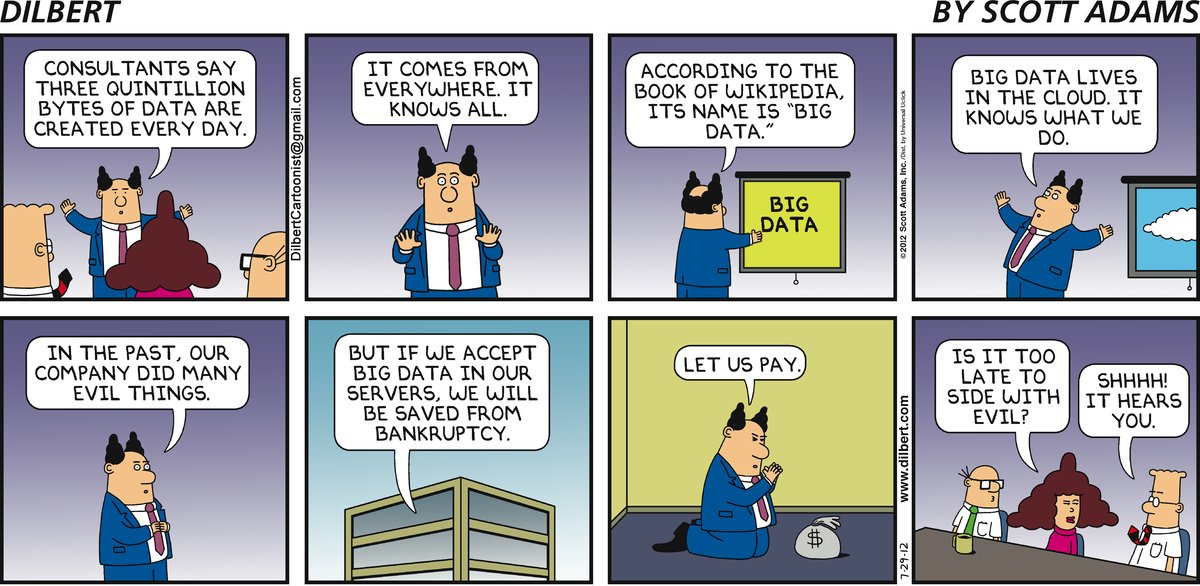
\includegraphics[width=0.985\textwidth]{img-presentation/dilbert}
\end{center}
\end{frame}

%%%%%%%%%%%%%%%%%%%%%%%%%%%%%%%%%%%%%%%%%%%%%%%%%%%%%%%%%%%%%%%%%%%%%%%%%%%%%%%%

\ignore{
\begin{frame}{}

\begin{center}
Dissertation Defense
\end{center}

\vspace{0.25in}

\begin{center}
\Huge
Divide and Conquer Algorithms 

for Faster Machine Learning
\end{center}

\vspace{0.25in}
\begin{center}
by Mike Izbicki
\end{center}
\end{frame}
}

\begin{frame}{Why faster machine learning?}

\vspace{0.05in}
\begin{tikzpicture}

%%%%%%%%%%%%%%%%%%%%%%%%%%%%%%%%%%%%%%%%

\node[text width=10cm] at (0,0) {
Facebook generates more than 200 terabytes of data per day (Facebook blog, 2014)
};

%\uncover<1>{
%\foreach \i in {1,...,20}
%\foreach \j in {1,...,10}
%{
    %\node at (0.5*\i-4.25,-2-0.5*\j) {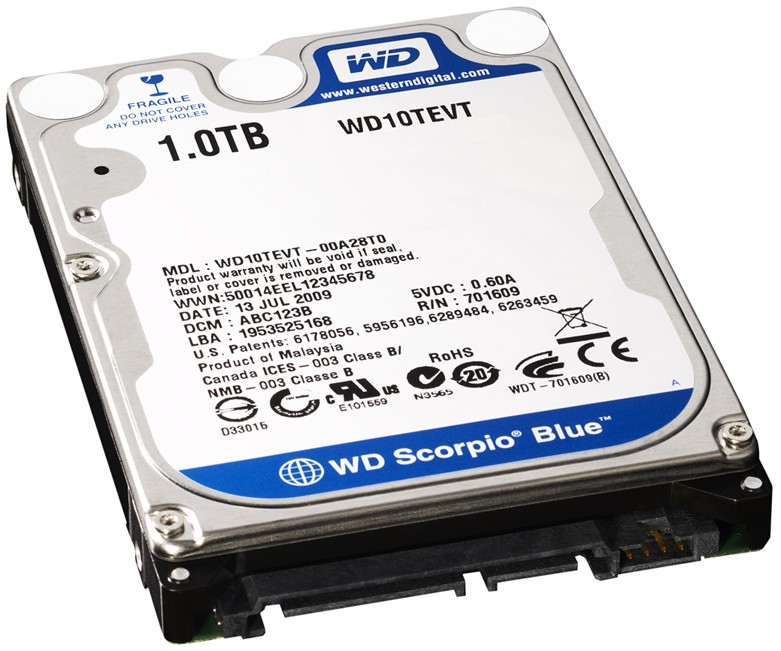
\includegraphics[width=0.4cm]{img-presentation/1tb}};
%}
%\node at (-4,-2) {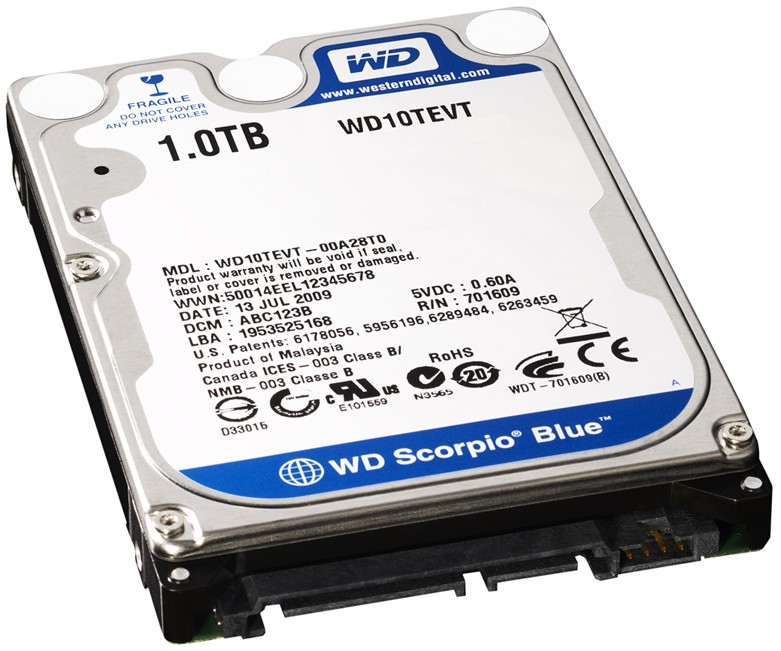
\includegraphics[width=3cm]{img-presentation/1tb}};
%}

%%%%%%%%%%%%%%%%%%%%%%%%%%%%%%%%%%%%%%%%

\uncover<2-9> {
\node at (-4.35,-0.9) {
\includegraphics[width=0.2cm]{img-presentation/dot}};
\node[text width=10cm] at (1,-0.9) {
    includes uploaded images%
    {\uncover<4-9>{, messages}}%
    {\uncover<5-9>{, and user likes}}
};
\uncover<2-6>{\node at (-2,-3.5) {
    %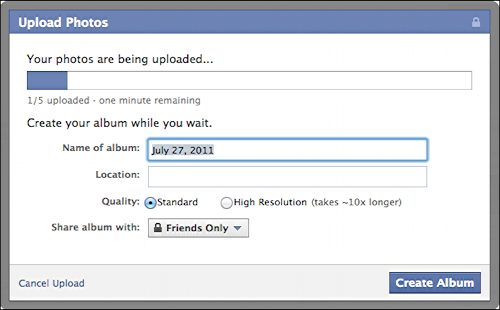
\includegraphics[width=5cm]{img-presentation/facebook-upload-photo-computer-6}
    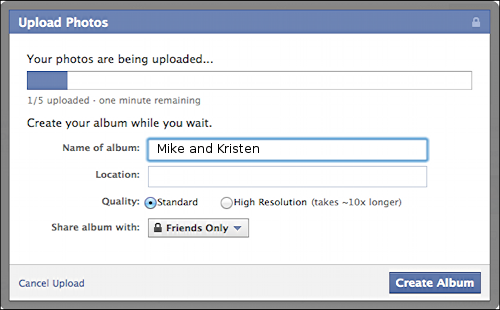
\includegraphics[width=5cm]{img-presentation/fb-upload}
};}
\uncover<2-6>{\node at (1.75,-3.75) {
    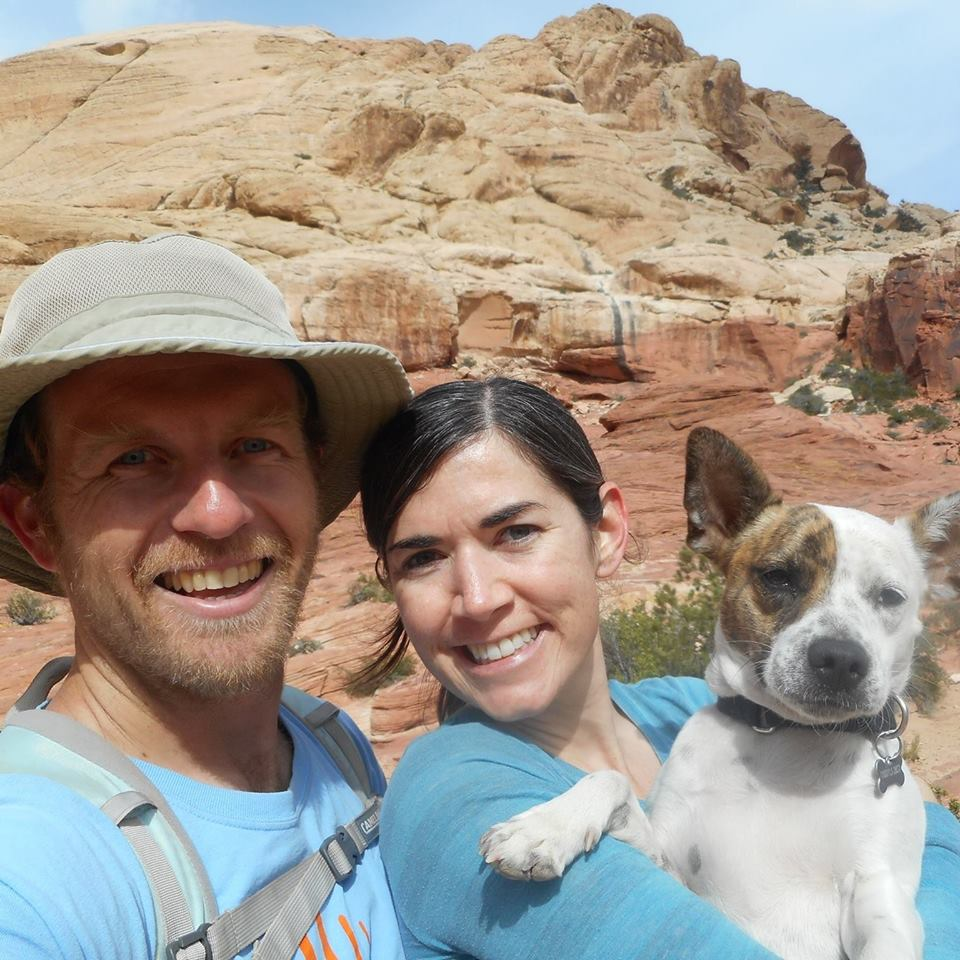
\includegraphics[width=3cm]{img-presentation/dog}
};}
\uncover<4-6>{\node at (5,-4.25) {
    %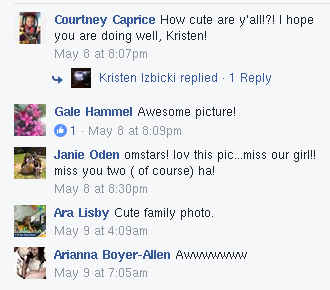
\includegraphics[width=3cm]{img-presentation/dog-message}
    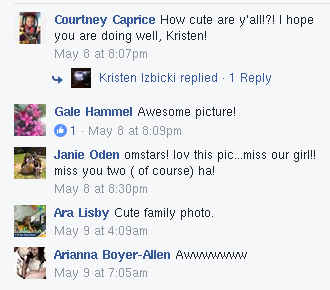
\includegraphics[width=4cm]{img-presentation/dog-message}
};}
\uncover<5-6>{\node at (3.5,-6.5) {
    
\includegraphics[width=3cm]{img-presentation/fb-like}
};}
}

%%%%%%%%%%%%%%%%%%%%%%%%%%%%%%%%%%%%%%%%

\uncover<6-9>{
\node at (-4.35,-1.5) {
\includegraphics[width=0.2cm]{img-presentation/dot}};
\node[text width=10cm] at (1,-1.5) {
    machine learning algorithms use this data to solve problems
};
\uncover<7-9>{
\node[text width=10cm] at (1,-2.0) {like identifying people in images
{\uncover<8-9>{and displaying profitable ads}}};
}

\uncover<7-8>{
\node at (-2,-5) {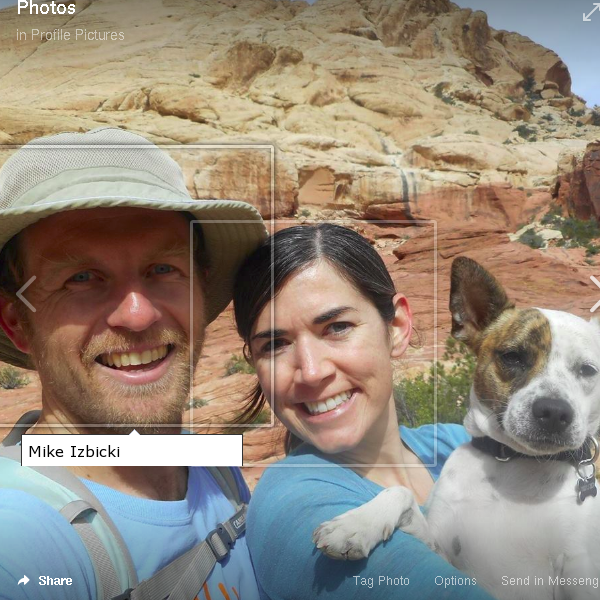
\includegraphics[width=5cm] {img-presentation/fb-faces2}};
}
\uncover<8>{\node at (4,-5) {
    
\includegraphics[width=5cm] {img-presentation/fb-ad-hiking}
};}
}

%%%%%%%%%%%%%%%%%%%%%%%%%%%%%%%%%%%%%%%%

\uncover<9> {
\node[text width=12cm] at (1,-2.6) {\textbf{Challenge:} we need new, faster algorithms to process this data};
%\node[text width=6cm] at (-2,-3.1) {Facebook has ``an estimated hundreds of thousands'' of computers};
%\node at (4,-5) {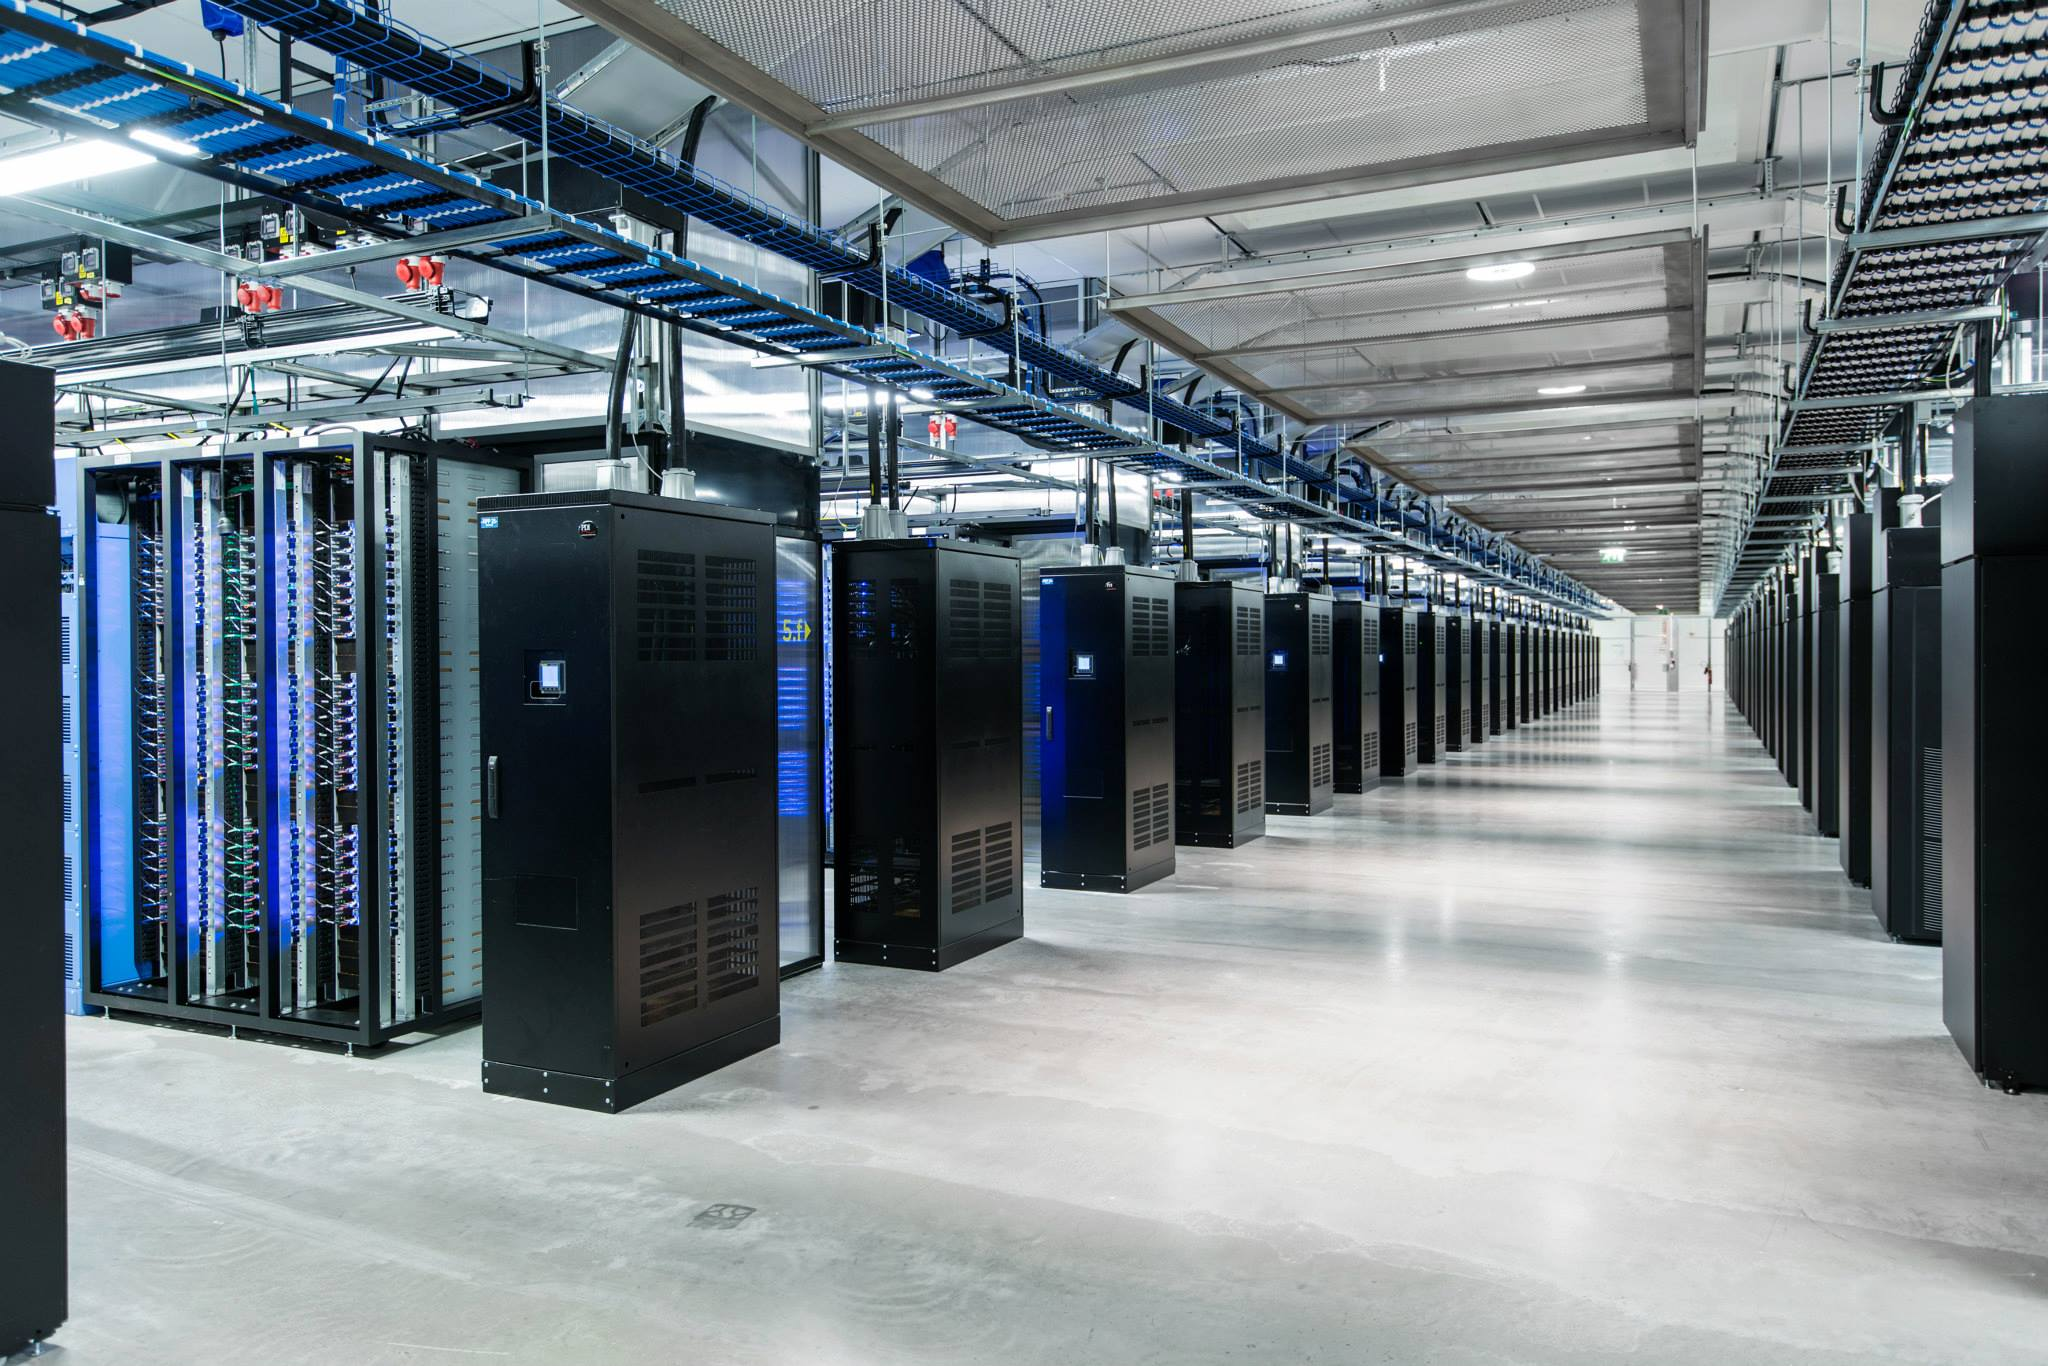
\includegraphics[width=6cm]{img-presentation/facebook_10969}};
}

%%%%%%%%%%%%%%%%%%%%%%%%%%%%%%%%%%%%%%%%

\end{tikzpicture}

%This data is stored on ``hundreds of thousands'' of computers
%
%(Facebook Datacenter FAQ)

\end{frame}

%%%%%%%%%%%%%%%%%%%%%%%%%%%%%%%%%%%%%%%%%%%%%%%%%%%%%%%%%%%%%%%%%%%%%%%%%%%%%%%%

\begin{frame}{Many organizations need faster machine learning}

\begin{itemize}
\item 
computer companies

\vspace{0.05in}
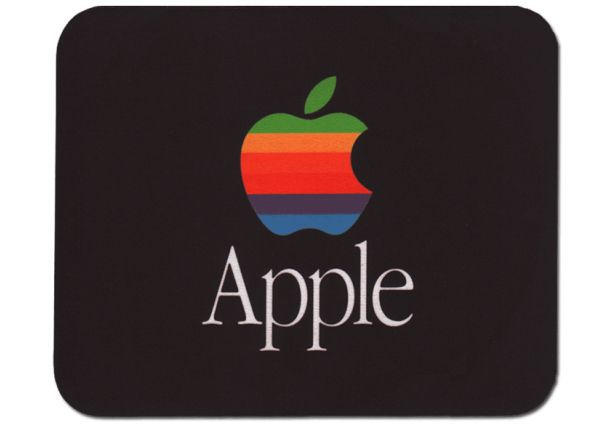
\includegraphics[height=1cm]{img-presentation/apple}~~~

\includegraphics[height=1cm]{img-presentation/ms}~~~

\includegraphics[height=1cm]{img-presentation/google}

\vspace{0.05in}

\includegraphics[height=1cm]{img-presentation/linkedin}~~~

\includegraphics[height=1cm]{img-presentation/yahoo}

\pause
\vspace{0.1in}
\item
traditional engineering

\vspace{0.05in}

\includegraphics[height=1cm]{img-presentation/pfizer}~~~

\includegraphics[height=1cm]{img-presentation/gm}

\pause
\vspace{0.1in}
\item 
pure scientific research

\vspace{0.05in}

\includegraphics[height=1cm]{img-presentation/nasa}~~~
%
\includegraphics[height=1cm]{img-presentation/nsf}~~~

\includegraphics[height=1cm]{img-presentation/cern}~~~

\includegraphics[height=1cm]{img-presentation/nih}

\end{itemize}

\end{frame}

%%%%%%%%%%%%%%%%%%%%%%%%%%%%%%%%%%%%%%%%%%%%%%%%%%%%%%%%%%%%%%%%%%%%%%%%%%%%%%%%

\begin{frame}{My research}
\textbf{Goal:} 
%Goal:
%\begin{itemize}
%\item
generic techniques that make machine learning faster for everyone

%for all these organizations
%\end{itemize}

\pause
\vspace{0.15in}
Examples
\begin{itemize}
\item
ad-click data from the Tencent search engine

(improve ad revenue for a given computational budget)

\vspace{-1.5cm}
\begin{tikzpicture}
\node at (0,0) {};
\node at (10,0) {
\includegraphics[width=2cm]{img-presentation/tencent}};
\end{tikzpicture}
%\vspace{-1cm}

\pause
\item
protein data bank

(first analysis of approximately 100,000 human 

proteins using random walk graph kernels)

\vspace{-1.5cm}
\begin{tikzpicture}
\node at (0,0) {};
\node at (9.5,0) {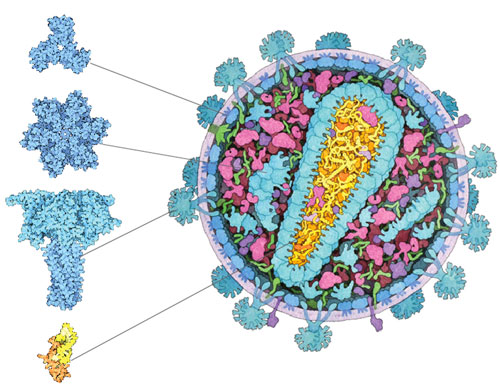
\includegraphics[width=2.5cm]{img-presentation/pdb}};
\end{tikzpicture}

\pause
\vspace{-0.4cm}
\item
Flickr creative commons images

(find patterns in 1.5 million images on a single machine)
\end{itemize}

\vspace{-0.8cm}
\begin{tikzpicture}
\node at (0,0) {};
\node at (11,0) {
\includegraphics[width=1.3cm]{img-presentation/flikr}};
\end{tikzpicture}

\pause
\vspace{-0.15in}
Main contributions are \textbf{theoretical} and \textbf{more general}
\end{frame}

\newcommand{\new}{(new)}

\begin{frame}{Outline of my contributions}

Mergeable learning algorithms
\begin{itemize}
    %\item simple example
    \item popular class of distributed learning algorithms
    \item fast cross validation algorithm
\end{itemize}

\vspace{0.1in}
Optimal weighted average (OWA) merge procedure
\begin{itemize}
    \item better theoretical guarantees than previous methods
    \item experiments on large scale ad-click data
\end{itemize}

\vspace{0.1in}
Cover tree data structure for nearest neighbor queries
\begin{itemize}
    \item merge procedure
    \item improved analysis of runtimes
    \item new notion of metric dimension 
    \item experiments on large scale protein and image data
\end{itemize}


%\vspace{-2in}
%\begin{tikzpicture}
%\node at (0,0) {};
%\node at (10,0) {
\includegraphics[width=2cm]{img-presentation/tencent}};
%\node at (9.5,-2.5) {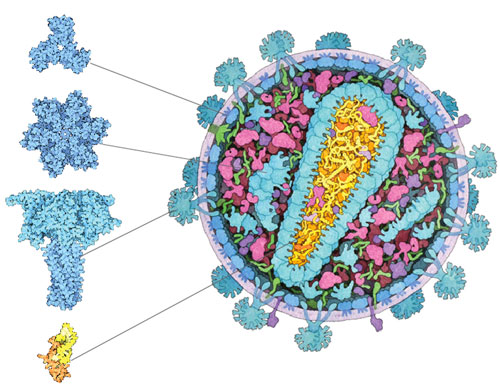
\includegraphics[width=2.5cm]{img-presentation/pdb}};
%\node at (11,-4) {
\includegraphics[width=1.3cm]{img-presentation/flikr}};
%\end{tikzpicture}

\end{frame}



\spacer{mergeable learning algorithms}
\begin{frame}{Mergeable learning algorithms overview}

\begin{itemize}
\Large
\item distributed machine learning with MapReduce
\item many existing algorithms fit this framework
\item simple ridge regression example
\item fast cross validation algorithm
\end{itemize}

\end{frame}




\tikzstyle{blackbox}=[shape=rectangle, draw, fill=black, draw=white, draw opacity=0, line width=0.15in, text=white, minimum size=0.3in]
\tikzstyle{whitebox}=[shape=rectangle, draw, fill=white, draw=black, minimum size=0.3in]

%%%%%%%%%%%%%%%%%%%%%%%%%%%%%%%%%%%%%%%%

\begin{frame}{Mergeable learning algorithms use 1 round of MapReduce}
\centering
\begin{tikzpicture}[line width=2pt]
\node[color=white] at (-6,-1) {\begin{sideways} partition \end{sideways}};
\node[minimum width=12cm,minimum height=1.7cm,fill=white,opacity=0.1] at (-0.5,-1) {};

\node (long) {\includegraphics[width=4in]{/home/user/docs/research/presentation_lib/dna/long}};

\uncover<1> {
\node at (-3,-1) {big data};
%\node at (-0.5,-3) {\rotatebox{90}{training}};
\node at (-1.1,-3) {{training}};
\node at (1.2,-5.8) {model};
}

\node[blackbox] (mc) [below of = long, node distance = 2.3in] {};

\draw[->,line width=2pt] (long) to (mc);


%%%%%%%%%%%%%%%%%%%%%%%%%%%%%%%%%%%%%%%
\pause
\node[minimum width=5in,minimum height=2.5in,fill=white] at (0,-1.05in) {};

\node at (-6,-1) {\begin{sideways} partition \end{sideways}};
\node[minimum width=12cm,minimum height=1.7cm,fill=green,opacity=0.1] at (-0.5,-1) {};

\node at (-6,-3) {\begin{sideways} map \end{sideways}};
\node[minimum width=12cm,minimum height=1.7cm,fill=green,opacity=0.1] at (-0.5,-3) {};

\node at (-6,-5) {\begin{sideways} reduce \end{sideways}};
\node[minimum width=12cm,minimum height=1.7cm,fill=green,opacity=0.1] at (-0.5,-5) {};

\node (long) {\includegraphics[width=4in]{/home/user/docs/research/presentation_lib/dna/long}};

\node (short1) at (-1.5in,-0.75in) {\includegraphics[width=1in]{/home/user/docs/research/presentation_lib/dna/short3}};
\node (short2) at (-0.5in,-0.75in) {\includegraphics[width=1in]{/home/user/docs/research/presentation_lib/dna/short2}};
\node (short3) at (0.5in,-0.75in) {\includegraphics[width=1in]{/home/user/docs/research/presentation_lib/dna/short1}};
\node (short4) at (1.5in,-0.75in) {\includegraphics[width=1in]{/home/user/docs/research/presentation_lib/dna/short2}};

\node[blackbox] (mc1) [below of=short1, node distance = 0.8in] {};
\node[blackbox] (mc2) [below of=short2, node distance = 0.8in] {};
\node[blackbox] (mc3) [below of=short3, node distance = 0.8in] {};
\node[blackbox] (mc4) [below of=short4, node distance = 0.8in] {};

\node[blackbox] at (-1.0125in,-2in) [out=270 ,in=180] (mc12) {};
\node[blackbox] at (1.0125in,-2in) (mc34) {};

\node[blackbox] (mc) [below of = long, node distance = 2.3in] {};

\draw[->] (-1.5in,-0.25in) to (-1.5in,-0.4in);
\draw[->] (-0.5in,-0.25in) to (-0.5in,-0.4in);
\draw[->] (0.5in,-0.25in) to (0.5in,-0.4in);
\draw[->] (1.5in,-0.25in) to (1.5in,-0.4in);
%\draw[->] (long) to (short1);
%\draw[->] (long) to (short2);
%\draw[->] (long) to (short3);

\draw[->] (short1) to (mc1);
\draw[->] (short2) to (mc2);
\draw[->] (short3) to (mc3);
\draw[->] (short4) to (mc4);

\draw[->] (mc1.south) to (mc12);
\draw[->] (mc2.south) to (mc12);
\draw[->] (mc3.south) to (mc34);
\draw[->] (mc4.south) to (mc34);

\draw[->] (mc12) to (mc);
\draw[->] (mc34) to (mc);

%\uncover<3>{
%\node[draw=red, line width = 2pt, fill=white, minimum width=4in, minimum height=1.5in] at (-0.1in,-0.4in) {
    %\parbox{3.5in}{
    %Computations over finite, constant-time monoids are complete in the parallel complexity class $\mathbb{NC}^1$.
%
    %$$
    %\mathbb{NC}^1 \subseteq \mathbb{NC} \subseteq \mathbb{P} \subseteq \mathbb{NP}
    %$$
    %}
%};}

\uncover<3> {
\node at (-0.5,-6.75) {\color{darkgreen} \textbf{
    Advantages: fast, implement with standard libraries, privacy 
}};
}

\uncover<4-5>{
\draw[color=red,line width=2pt,fill=lightred, opacity=0.5] (-2.55,-4.3) ellipse (2cm and 1.3cm);
\draw[color=red,line width=2pt                           ] (-2.55,-4.3) ellipse (2cm and 1.3cm);

\node at (-3.3,-6.3) {\color{red} \textbf{
    How do we merge two models?
    }};
}

\uncover<5> {
\node at (-3.1,-6.9) {\color{red} \textbf{What else does merging give us?}};
}

\onslide<1->
\end{tikzpicture}
\end{frame}


%%%%%%%%%%%%%%%%%%%%%%%%%%%%%%%%%%%%%%%%%%%%%%%%%%%%%%%%%%%%%%%%%%%%%%%%%%%%%%%


\begin{frame}{Mergeable estimators are popular}
    \vspace{0.4in}
    \uncover<2>{
    
\begin{tikzpicture}
        \draw[draw=white,opacity=0.75,fill=yellow] (0,0) -- (12.25,0) -- (12.25,1.55) -- (0,1.55);
    \end{tikzpicture}
}
    \vspace{-1.275in}

    \setstretch{0.8}{
\begin{itemize}
    \item
    methods with closed form solution
    %(\textbf 3 solutions)

    {\tiny linear exponential families, naive bayes, ridge regression}

    \vspace{0.1in}
    \item 
    regularized loss minimization
    %(\textbf 9 solutions)

    {\tiny (Mergu and Ghosh, 2003; McDonald et al., 2009; Zinkevich et al., 2010; Zhang et al., 2012, 2013b; Liu and Ihler, 2014; Battey et al., 2015; Han and Liu, 2016; Lee et al., 2017)}

    \vspace{0.1in}
    \item 
    principle component analysis
    %(\textbf 2 solutions)

    {\tiny (Qu et al., 2001; Liang et al., 2013)}

    \vspace{0.1in}
    \item 
    submodular optimization
    %(\textbf 6 solutions)
    
    {\tiny (Mirzasoleiman et al., 2013; Barbosa et al., 2015; Malkomes et al., 2015; Bhaskara et al., 2016; Barbosa et al., 2016; Mirzasoleiman et al., 2016)}

    \vspace{0.1in}
    \item 
    variational inference
    %(\textbf 3 solutions)

    {\tiny (Broderick et al., 2013; Campbell and How, 2014; Neiswanger et al., 2015)}

    \vspace{0.1in}
    \item 
    markov chain monte carlo
    %(\textbf 8 solutions)
    
    {\tiny (Wang and Dunson, 2013; Minsker et al., 2014; Neiswanger et al., 2014; Wang et al., 2015; White et al., 2015; Srivastava et al., 2015; Nemeth and Sherlock, 2016; Scott et al., 2016)}
\end{itemize}
}
\end{frame}

\begin{frame}{The regularized loss minimization (RLM) framework}

Solve the following optimization
\begin{equation}
\wmle = \argmin_{\w\in\W} \sum_{(y,\x)\in Z} \loss(y;\trans\w\x) + \lambda\reg(\w)
\end{equation}
where
\begin{itemize}
\item $Z$ is a dataset with $mn$ points ($m$ machines each with $n$ points)
\item $y\in\Y\subset\mathbb R$
\item $\x\in\X\subset\mathbb R^d$
\item $\w\in\W\subset\mathbb R^d$
\item $\loss$ is the (not necessarily convex) loss function
\item $\reg : \W\to\mathbb R$ is the regularization function
\end{itemize}

\vspace{0.15in}
\textbf{Theory:} the statistical error decays as $\ltwo{\wstar-\wmle} \le O(\sqrt{d/mn})$ where $\wstar$ is the optimal parameter in $\W$.
\end{frame}

%%%%%%%%%%%%%%%%%%%%%%%%%%%%%%%%%%%%%%%%

\begin{frame}{RLM for ridge regression can be exactly parallelized}
In ridge regression, we set
\begin{equation}
\loss(\y,\trans\w\x) = \ltwo{\y-\trans\w\x}^2 
~~~ \text{and} ~~~
\reg(\w) = \ltwo{\w}^2,
\end{equation}
so the estimator has closed form solution
\begin{equation}
\wmlerr = (\trans X X - \lambda I)^{-1}(\trans X Y),
\end{equation}
where $X : \R^{mn\times d}$ and $Y : \R^{mn\times 1}$ are the design and response matrices.

\pause
\hrulefill
\vspace{0.1in}

In the \textbf{map} phase, each machine $i$ calculates
\begin{equation}
A_i = \trans X_i X_i
~~~\text{and}~~~
B_i = \trans X_i Y_i
\end{equation}
where $X_i : \R^{n\times d}$ and $Y : \R^{n\times 1}$ are the design and response matrices for only the data on machine $i$.
In the \textbf{reduce} phase, calculate
\begin{equation}
\textstyle
\wmlerr = \left(\sum_{i=1}^m A_i - \lambda I\right)^{-1}\left(\sum_{i=1}^m B_i\right).
\end{equation}
\end{frame}

\renewcommand{\arraystretch}{1}

\newcommand{\h}[1]{\textup{\lstinline{#1}}}
\lstnewenvironment{code}
    %{\lstset{}%
      %\csname lst@SetFirstLabel\endcsname}
    %{\csname lst@SaveFirstLabel\endcsname}
    {
    \lstset{
      basicstyle=\small\ttfamily,
      xleftmargin=\parindent,
      xleftmargin=\parindent,
      flexiblecolumns=false,
      keepspaces=true,
      frame=single,
      basewidth={0.5em,0.45em},
      literate={+}{{$+$}}1 {/}{{$/$}}1 {*}{{$*$}}1 {=}{{$=$}}1
               {>}{{$>$}}1 {<}{{$<$}}1 {\\}{{$\lambda$}}1
               {\\\\}{{\char`\\\char`\\}}1
               {->}{{$\rightarrow$}}2 {>=}{{$\geq$}}2 {<-}{{$\leftarrow$}}2
               {<=}{{$\leq$}}2 {=>}{{$\Rightarrow$}}2 
%                {\ .}{{$\circ$}}2 {\ .\ }{{$\circ$}}2
               {>>}{{>>}}2 {>>=}{{>>=}}2
               {|}{{$\mid$}}1               
               {<>}{{$\diamond$}}1          
               {++}{{$\+$}}1                
               {mempty}{{$\epsilon$}}1               
               {Theta}{{$\Theta$}}1               
    }
    }
    {}

\newcommand{\set}[1]{\ensuremath{\mathcal{{#1}}}}
%\newcommand{\vector}[1]{\textbf{{{#1}}}}
\newcommand{\elem}[1]{\textbf{{#1}}}
\newcommand\op{\ensuremath{\diamond}}
\newcommand\id{\ensuremath{\mathbf{epsilon}}}
\newcommand\+{\op}
%\newcommand\+{\mdoubleplus}
\newcommand\doubleplus{+\kern-1.3ex+\kern0.8ex}
\newcommand\mdoubleplus{\ensuremath{\mathbin{+\mkern-10mu+}}}

%%%%%%%%%%%%%%%%%%%%%%%%%%%%%%%%%%%%%%%%%%%%%%%%%%%%%%%%%%%%%%%%%%%%%%%%%%%%%%%

\begin{frame}[fragile]{Merging gives us: fast cross-validation}

traditional pseudocode:
\begin{code}
for i = 1..n
    let test_datapoint = i_th datapoint in dataset
    let train_dataset  = dataset - test_datapoint

    train on train_dataset  
    infer on test_datapoint
    calculate loss        

return mean and stddev of losses
\end{code}

%running time: $\Theta\left(k (t(n-\frac{n}{k}) +  i(\frac{n}{k}) + \frac{n}{k})\right)$
%\vspace{0.15in}
%running time: $\Theta(nt(n-1) + ni(1))$
%\vspace{0.15in}

\vspace{0.1in}
traditional run times:
\vspace{0.1in}

\centering
\begin{tabular}{l|cc|cc}
%\hline
& training & inference & LOO cv & $k$-fold cv \\ %leave-one-out \\ 
%algorithm & t(n) & i(1) & overall \\ %leave-one-out \\ 
\hline
ridge regression & $O(n)$ & $O(1)$ & $O(n^2)$ & $O(kn)$ \\
%\hline
%naive bayes (normal dist) & $O(n)$ & $O(1)$ & $O(n^2)$ \\
%$k$-nn (cover tree) & $O(n\log n)$ & $O(\log n)$ & $O(n^2\log n)$ \\
%\hline
\end{tabular}

\end{frame}

\begin{frame}[fragile]{Merging gives us: fast cross-validation}

\begin{tikzpicture}

\node at (0.775in,2) {
    \includegraphics[width=1.6in]{/home/user/docs/research/presentation_lib/dna/long}
};

\foreach \i in {0,1,...,10} {
    %\node[draw,minimum size=0.15in] at (\i*0.15in,1.5) {};
    \uncover<2->{
    \node[fill=black,minimum size=0.15in,draw=white,line width=1pt] at (\i*0.15in,1) {};
    }
}

\uncover<3->{
\foreach \i in {1,...,9} {
    %\foreach \j in {0,...,\i} {
        %\node[fill=black,minimum size=0.15in,draw=white,line width=1pt] at (\j*0.15in,-\i*0.375-0.375) {};
        \node[fill=black,minimum height=0.15in,minimum width=\i*0.15in,draw=white,line width=1pt] at (\i*0.075in-0.075in,-\i*0.375) {};
    %}
}
}

\uncover<4->{
\foreach \i in {0,...,9} {
    %\foreach \j in {\i,...,9} {
        %\node[fill=black,minimum size=0.15in,draw=white,line width=1pt] at (\j*0.15in+0.15in,-\i*0.375) {};
        \node[fill=black,minimum height=0.15in,minimum width=1.5in-\i*0.15in,draw=white,line width=1pt] at (\i*0.075in+0.825in,-\i*0.375) {};
    %}
}
}

\uncover<2>{\node[minimum width=2.8in,minimum height=0.35in,fill=green,opacity=0.2] at (3.2in,0.85in) {};}
\uncover<3>{\node[minimum width=2.8in,minimum height=0.5in,fill=green,opacity=0.2] at (3.2in,0.25in) {};}
\uncover<4>{\node[minimum width=2.8in,minimum height=0.5in,fill=green,opacity=0.2] at (3.2in,-0.4in) {};}
\uncover<5>{\node[minimum width=2.8in,minimum height=0.65in,fill=green,opacity=0.2] at (3.2in,-1.15in) {};}

\node[text width=2.8in] at (3.2in,-1) {
\begin{code}
for i = 1..n
    m[i] <- train on dp[i]

prefix[1] = empty
for i = 2..n
    prefix[i]=merge(prefix[i-1],m[i-1])

suffix[n] = empty 
for i = n-1..1
    suffix[i]=merge(suffix[i+1],m[i+1])

for i = 1..n
    m <- merge(prefix[i], suffix[i])
    infer on dp i with m   
    calculate loss

return mean and stddev of losses
\end{code}

%\begin{tikzpicture}
%\node[draw] {
%\lstinline{calculate prefixes   -- time n*t(n)}
%\lstinline{calculate suffixes   -- time n*t(n)}
%%\lstinline{}
%\lstinline{for i = 1..n}
%\lstinline{    merge rows           -- time n*beta(n)}
%\lstinline{    inference            -- time n*i(1)}

%};
%\end{tikzpicture}
};

\end{tikzpicture}

%\vspace{0.15in}
\end{frame}


%%%%%%%%%%%%%%%%%%%%%%%%%%%%%%%%%%%%%%%%%%%%%%%%%%%%%%%%%%%%%%%%%%%%%%%%%%%%%%%

\renewcommand{\arraystretch}{1.5}
\begin{frame}{Fast cross-validation summary}
%\footnotesize
\begin{center}
%\begin{tabular}{l|ccc|cc}
%\hline
%algorithm & training & inference & monoid & standard cv & fast cv \\
%%algorithm & $t(n)$ & $i(n)$ & $\beta(n)$ & standard & monoid \\
%\hline
%\hline
%normal distribution & $\Theta(n)$ & $\Theta(1)$ & $\Theta(1)$ & $\Theta(n^2)$ & $\Theta(n)$ \\
%kernel density & $\Theta(n\log n)$ & $\Theta(\log n)$ & $\Theta(n)$ & $\Theta(n^2\log n)$ & $\Theta(n^2)$ \\
%\hline
%\end{tabular}

    Assuming merging takes constant time (as in ridge regression), then:
    \vspace{0.30in}

%\begin{tikzpicture}[node distance=2.5cm, auto, >=stealth]
%
%\node at (1.4in,1.5in) {
\begin{tabular}{l|cc}
%\hline
& LOO cv & $k$-fold cv \\
%algorithm & $t(n)$ & $i(n)$ & $\beta(n)$ & standard & monoid \\
%\hline
\hline
standard & $O(n^2)$ & $O(kn)$ \\
fast & $O(n)$ & $O(n)$ \\
%\hline
%\uncover<3->{abelian group cv & $O(n)$ & $O(n\log n)$ } \\
%\uncover<4->{double monoid cv & --- & $O(n\log n)$ } \\
%\hline
\end{tabular}

\vspace{0.3in}
Also works when merging takes non-constant time

(but more complicated runtime expressions)
%};
%\uncover<1>{ \node[fill=white,minimum width=4.5in,minimum height=2in] at (1.4in,0.5in) {}; }
%\uncover<2,3>{ \node[fill=white,minimum width=4.5in,minimum height=1in] at (1.4in,0.5in) {}; }

%\begin{tabular}{l|cccc}
%\hline
%algorithm & standard cv & monoid cv  & abelian group cv & double monoid cv\\
%%algorithm & $t(n)$ & $i(n)$ & $\beta(n)$ & standard & monoid \\
%\hline
%\hline
%normal distribution & $O(n^2)$ & $O(n)$ & $O(n)$ & $O(n)$ \\
%kernel density & $O(n^2\log n)$ & $O(n^2)$ & $O(n\log n)$ & $O(n\log n)$ \\
%\hline
%\end{tabular}

%\uncover<1->{
%\node[blackbox] (dataset) [minimum height=0.3in] {data set};
%\node[blackbox] (model)   [minimum height=0.3in, node distance=1.5in,right of = dataset] {model};
%\node[blackbox] (answer)  [minimum height=0.3in, node distance=1.5in,right of = model] {result};
%\draw[->,line width=2pt] (dataset) to node[above] {\h{train}} (model);
%\draw[->,line width=2pt] (model) to node[above] {\h{inference}} (answer);
%}
%
%\uncover<2>{
%\node (l1) [color=blue] at (-0.1,-1.3) {free monoid};
%\node (l2) [color=blue] at (2,1.3) {homomorphism};
%\node (l3) [color=blue] at (4,-1.3) {monoid};
%
%\draw[->,color=blue,ultra thick] (l1) to (dataset);
%\draw[->,color=blue,ultra thick] (l2) to (2,0.5);
%\draw[->,color=blue,ultra thick] (l3) to (model);
%}
%
%
%\uncover<3>{
%\node (l1) [color=blue] at (-0.1,-1.3) {free abelian group};
%\node (l2) [color=blue] at (2,1.3) {homomorphism};
%\node (l3) [color=blue] at (4,-1.3) {abelian group};
%
%\draw[->,color=blue,ultra thick] (l1) to (dataset);
%\draw[->,color=blue,ultra thick] (l2) to (2,0.5);
%\draw[->,color=blue,ultra thick] (l3) to (model);
%}
%
%\uncover<4>{
%\node (l1) [color=blue] at (-0.1,-1.3) {free monoid};
%\node (l2) [color=blue] at (1.9,1.3) {homomorphism};
%\node (l3) [color=blue] at (4,-1.3) {monoid};
%\node (l4) [color=blue] at (5.8,1.3) {homomorphism};
%\node (l5) [color=blue] at (8,-1.3) {monoid};
%
%\draw[->,color=blue,ultra thick] (l1) to (dataset);
%\draw[->,color=blue,ultra thick] (l2) to (2.1,0.5);
%\draw[->,color=blue,ultra thick] (l3) to (model);
%\draw[->,color=blue,ultra thick] (l4) to (5.6,0.5);
%\draw[->,color=blue,ultra thick] (l5) to (answer);
%}
%
%\end{tikzpicture}
\end{center}
\end{frame}
\renewcommand{\arraystretch}{1}



\spacer{the optimal weighted average}
\begin{frame}{Optimal weighted average overview}

\begin{itemize}
\Large
\item naive averaging estimator
\begin{itemize}
\Large
\item simple
\item poor statistical guarantees
\end{itemize}
\item (full) optimal weighted average
\item good statistical guarantees
\item experiments
\begin{itemize}
\Large
\item synthetic data
\item large scale ad-click data
\end{itemize}
\end{itemize}

\end{frame}



\begin{frame}{The averaging distributed estimator}

Procedure:

\begin{itemize}

%\item Assign to each machine $i\in\{1...m\}$ a dataset $Z_i$ with $n$ datapoints

\item In the \textbf{map} phase, each machine calculates the local ERM

\begin{equation}
\wmle_i = \argmin_{\w} \sum_{(y,\x)\in Z_i} \loss(y;\trans\w\x) + \lambda\reg(\w)
\end{equation}

where $Z_i$ is the local data set of machine $i$.

%\item A central server calculates the averaging estimator

\item
In the \textbf{reduce} phase, we calculate
\begin{equation}
\wave = \frac{1}{m}\sum_{i=1}^m \wmle_i
.
\end{equation}

\end{itemize}

\textbf{Theory:}

\vspace{-0.2in}
\begin{equation}
\ltwo{\wstar-\wave} \le 
\ltwo{\wstar-\E\wave} 
+
\ltwo{\E\wave-\wave} 
\end{equation}

\hspace{1.9in}
$O(\sqrt{d/n})$
\hspace{0.3in}
$O(\sqrt{d/mn})$

\vspace{0.15in}
(McDonald et al., 2009; Zhang et al., 2012; Rosenblatt and Nadler, 2016)
\end{frame}

%%%%%%%%%%%%%%%%%%%%%%%%%%%%%%%%%%%%%%%%

\begin{frame}{Can we do better than averaging? Yes!}

Estimators with bias reduction
\begin{itemize}
%\item
%If the datasets on each machine overlap each other, then there is a reduction in bias
%(Zinkevich et al., 2012)
%
%\textcolor{darkgreen}{Good: simple}
%; 
%\textcolor{red}{Bad: different problem setup}

\item
Estimate the bias via a bootstrap subsample (Zhang et al., 2012)

\textcolor{darkgreen}{easy to implement}
; 
\textcolor{red}{suboptimal scalability}

\item
Closed form formula for the optimal $\lambda$ in kernel ridge regeression (Zhang et al., 2013)

\textcolor{darkgreen}{easy to implement}
; 
\textcolor{red}{applies to limited models}

\item
Closed form estimates of the bias in certain L1 penalized models

(Lee et al., 2015; Battey et al., 2015)

\textcolor{darkgreen}{easy to implement}
; 
\textcolor{red}{applies to limited models}

\item
Averaging the models with the KL average (Liu and Ihler, 2014)

\textcolor{darkgreen}{good statistical guarantees}
; 
\textcolor{red}{must solve intractable integral}

\end{itemize}

\pause

Goal: 
\begin{itemize}
    \item easy to implement 
    \item good statistical guarantees 
    \item efficiently calculatable
\end{itemize}

%\vspace{0.15in}
%Impossibility theorems
%
%\begin{itemize}

%\item
%At least $\Omega(m\min\{n,d\})$ bits must be transferred for $O(\sqrt{d/mn})$ error rate
%(Braverman et al., 2016)

%\item
%No merged estimator can achieve $O(\sqrt{d/mn})$ error rate
%
%(Zhang et al. 2013; Shamir 2014; Garg et al. 2014; Liu and Ihler 2014)\!\!\!\!
%
%%\begin{itemize}
%\item
%All results assume that the merge procedure does not depend on data
%%\end{itemize}
%
%\end{itemize}

\end{frame}



%%%%%%%%%%%%%%%%%%%%%%%%%%%%%%%%%%%%%%%%

\begin{frame}
\frametitle{The \uncover<1-6>{full} optimal weighted average (OWA)}

Procedure:
\uncover<2-7>{
\vspace{0.1in}
\begin{itemize}
\item
In the \textbf{map} phase,
calculate the $\wmle_i$ as before
}

\uncover<3-7>{
\vspace{0.1in}
\item
In the \textbf{reduce} phase,
%On the second round, 
\begin{itemize}
\item 
Let $\Wowa = \vecspan\{\wmle_i\}_{i=1}^m$\uncover<7>{, $Z^{owa}$ be a new dataset}
}

\uncover<4-7>{
\item Calculate
\begin{align}
\label{eq:afull}
\wowa{}^{\uncover<1-6>{,full}} &= \argmin_{\w\in\Wowa} \sum _{(\x,y)\in Z^{\textit{\uncover<7>{owa}}}} \loss\left(y,\trans\x\w \right)
+
\lambda \reg(\w)
\end{align}
}
\end{itemize}
\end{itemize} 

%\vspace{0.1in}
Graphical Intuition
\begin{center}
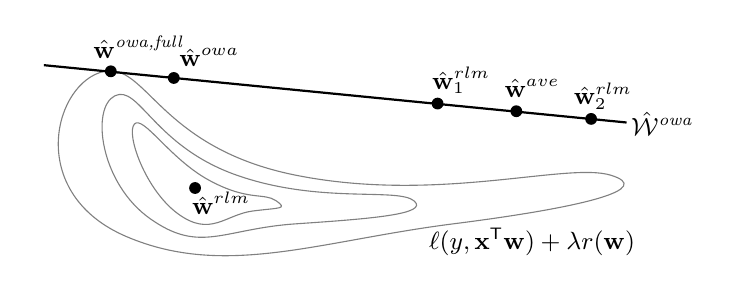
\begin{tikzpicture}
    [
    dot/.style = {minimum width=0.15cm,inner sep=0pt,line width=0pt,fill,circle,black,font=\small}
    , yscale=0.65
    ]
\small
\draw[gray] plot [smooth cycle,tension=1] coordinates {(-0.5,-0.75) (-1.05,1) (-0.1,-0.1) (0.75,-0.5) (0.45,-0.7) };
\draw[gray] plot [smooth cycle,tension=1] coordinates {(-0.85,-0.85) (-1.3,1.55) (0.25,0) (2.5,-0.5) (1,-0.95)};
\draw[gray] plot [smooth cycle,tension=1] coordinates {(-1.15,-1.2) (-1.5,2) (1,0) (5,0) (3,-0.95)};

\node[dot] (wstar) at (-0.28,-0.25) {};
\node at (0.05,-0.55) {$\wmle$};

\uncover<3-7>{
\draw[thick] (-2.2,2.15) -- (5.2,1.03);
\node at (5.65,1.0) {$\Wowa$};
}

\uncover<2-7>{
%\node[dot] (wstarproj) at (0.1,1.8) {};
%\draw (wstar) -- (wstarproj);
%\draw (0.07,1.65) -- (0.23,1.62) -- (0.26,1.78);

%\node[dot] (wavestar) at (4,0.5) {};
%\node                 at (4.5,0.3) {$\E\wave$};
\node[dot] (wave) at (2.80,1.40) {};
\node at (3.1,1.85) {$\wmle_1$};
\node[dot] (wave) at (4.75,1.10) {};
\node at (4.9,1.55) {$\wmle_2$};
%\node[dot] (wave) at (3.8,1.25) {};

}

\uncover<4-7>{
\node[dot] at (-1.35,2.03) {};
\node at (-1.0,2.5) {$\wowafull$};
}

\uncover<6-7>{
\node[dot] (wave) at (3.8,1.25) {};
\node at (4.0,1.7) {$\wave$};
}

\uncover<7>{
\node[dot] at (-0.55,1.9) {};
\node at (-0.1,2.3) {$\wowa$};
}

\node at (4,-1.3) {$\loss(y,\trans\x\w)+\lambda \reg(\w)$};
%\node at (6.95,1.0) {$\Wowa = \vecspan\{\wmle_i\}_{i=1}^m$};

\end{tikzpicture}
\end{center}

\end{frame}

%%%%%%%%%%%%%%%%%%%%%%%%%%%%%%%%%%%%%%%%

\begin{frame}{Efficiently calculating $\wowa$}

%Let $\matW = \bigg(\wmle_1, \wmle_2, ..., \wmle_m\bigg) \in \mathbb R^{d\times m}$
%
%\vspace{0.1in}
%Then every $\w\in\Wowa$ can be written as $\w=\matW\alpha$, where $\alpha\in\mathbb R^m$

\vspace{0.1in}
We can rewrite $\wowa$ as
%$\wowa = \matW \ahat$
%where
\begin{align}
\wowa &= \matW \ahat
\\
\label{eq:afull}
\ahat &= \argmax_{\alpha\in\mathbb R^m} \sum _{(\x,y)\in \Zowa} \loss\left(y,\trans\x \matW \alpha \right)
+
\lambda \reg(\matW\alpha)
\\
\matW &= \bigg(\wmle_1, \wmle_2, ..., \wmle_m\bigg) \in \mathbb R^{d\times m}
\end{align}

%In the second round of communication
%\begin{itemize}
%\item Each machine transmits $\trans\x\matW$ for each data point in $\Zowa$
%\item This is $O(m)$ bits per data point 
%
%~~~~~~~~~$O(m\nowa)$ bits per machine
%
%~~~~~~~~~$O(m^2\nowa)$ bits total
%%\item Whenever $m\nowa < d$, fewer bits are transfered than the first round
%\end{itemize}

\pause
Notice that:
\begin{itemize}
%\item
%The merging procedure depends on the data,
%so existing impossibility theorems do not apply.

%\pause
\item
The $\ahat$ optimization happens in a low dimensional subspace, so few datapoints are needed.

\pause
\item
The $\trans\x\matW$ in $(11)$ does not depend on $\alpha$, so needs to be computed only once (instead of each iteration).

%\pause
%\item
%The $\Zowa$ dataset should be stored already on the reduce server.
%
%(In the paper, we provide an algorithm for efficiently communicating the $\Zowa$ dataset to the reducer if needed.)

\end{itemize}

\end{frame}



\newtheorem*{sgt}{The subgaussian tail condition}
\newtheorem*{thm1}{Theorem 1: error of $\wowafull$}
\newtheorem*{thm2}{Theorem 2: error of $\wowa$}

\pgfmathdeclarefunction{gauss}{2}{%
  \pgfmathparse{1/(#2*sqrt(2*pi))*exp(-((x-#1)^2)/(2*#2^2))}%
}

\pgfmathdeclarefunction{multi}{2}{%
    \pgfmathparse{(0.0001+abs(sin((x-0.2)/100)))*1/(#2*sqrt(2*pi))*exp(-((x-0.4)^2)/(2*#2^2))}%
}

\pgfmathdeclarefunction{truncated}{2}{%
    \pgfmathparse{(abs(x)<1.5)*1/(#2*sqrt(2*pi))*exp(-((x-#1)^2)/(2*#2^2))}%
}

\newcommand{\mkdensity}[2]{
\begin{axis}[
  no markers, 
  domain=-3.5:3.5, 
  samples=100,
  axis lines=left, 
  xlabel=$\ltwo{\wstar-\wmle_i}$,
  every axis y label/.style={at=(current axis.above origin),anchor=south},
  every axis x label/.style={at=(current axis.right of origin),anchor=west},
  height=4.5cm, 
  width=10cm,
  xtick=0, 
  ytick=\empty,
  enlargelimits=false, 
  clip=false, 
  axis on top,
  grid = major
  ]
%\addplot [very thick,cyan!50!black] {gauss(0, 1)};
  \addplot [very thick,cyan!50!black] {{#2}};
\end{axis}
\node[text width=10cm] at (4,3.5) {Example: {#1}};
\node at (-0.5,1.5) {\rotatebox{90}{density}};
}

\begin{frame}{OWA's theoretical analysis}

%%%%%%%%%%%%%%%%%%%%%%%%%%%%%%%%%%%%%%%%

\begin{sgt}
%Let $\wmle_i$ be a linear estimator trained on $n$ data points of dimension $d$.
Let $t>0$.
Then, for each machine $i$, with probability at least $1-\exp(-t)$,
\begin{equation}
%\ltwo{\wstar-\what} \le O\left( \sqrt\frac {dt} {n} \right)
\ltwo{\wstar-\wmle_i} \le O\left( \sqrt{dt/n} \right)
.
\label{eq:sgt}
\end{equation}
\end{sgt}

%%%%%%%%%%%%%%%%%%%%%%%%%%%%%%%%%%%%%%%%

\begin{center}
\begin{tikzpicture}
\uncover<2>{\mkdensity{standard gaussian distribution}{gauss(0,1)}}
\uncover<3>{\mkdensity{truncated gaussian distribution}{truncated(0,1)}}
\uncover<4>{\mkdensity{biased gaussian distribution}{gauss(1.5,1)}}
\uncover<5>{\mkdensity{multimodal distributions}{multi(0,1)}}
\end{tikzpicture}
\vspace{-1.8in}
\end{center}

%%%%%%%%%%%%%%%%%%%%%%%%%%%%%%%%%%%%%%%%

\vspace{0.15in}
\uncover<6>{
This is a mild condition known to hold in many situations of interest.

\begin{itemize}
\item
In the asymptotic regime as $n\to\infty$,
\begin{equation}
\sqrt{n}\ltwobig{\I^{-1/2}(\wstar-\wmle_i)} \law \normal{0}{I}
\end{equation}
where $\I$ is the Fisher information matrix.
The loss $\loss$ may be nonconvex,
and the data may even be non-i.i.d.\
(Le Can, 1960).

\item
Similar results hold in the finite sample regime (Spokoiny, 2012).

\item
Important: biased estimators satisfy this condition!
\end{itemize}
    \vspace{-1.8in}
}

%%%%%%%%%%%%%%%%%%%%%%%%%%%%%%%%%%%%%%%%

\uncover<7-8>{
\begin{thm1}
\label{theorem:wowafull}
%Assume the Hessian Condition and that the $\wmle_i$s satisfy the SGT condition.
Let $t>0$.
Then with probability at least $1-\exp(-t)$, 
\begin{equation}
%\ltwo{\wowafull-\wstar} \le \sqrt{\frac{\qhi}{\qlo}}\ltwo{\proj{\Wowa}\wstar}
%\ltwo{\wowafull-\wstar} \le \sqrt{\frac{\qhi}{\qlo}}\sqrt{\frac{v_t}{n}}
\ltwo{\wstar-\wowafull} \le O\left(
%\sqrt{\frac{dt}{mn}}
\sqrt{{dt}/{mn}}
\right)
.
\end{equation}
\end{thm1}
}

%%%%%%%%%%%%%%%%%%%%%%%%%%%%%%%%%%%%%%%%

\uncover<8>{
    %\vspace{-2in}
\begin{thm2}
\label{theorem:wowafull}
%Assume the Hessian Condition and that the $\wmle_i$s satisfy the SGT condition.
Let $t>0$ and $\nowa=mn/d$.
Then with probability at least $1-\exp(-t)$, 
\begin{equation}
%\ltwo{\wowafull-\wstar} \le \sqrt{\frac{\qhi}{\qlo}}\ltwo{\proj{\Wowa}\wstar}
%\ltwo{\wowafull-\wstar} \le \sqrt{\frac{\qhi}{\qlo}}\sqrt{\frac{v_t}{n}}
\ltwo{\wstar-\wowa} \le O\left(
%\sqrt{\frac{dt}{mn}}
\sqrt{{dt}/{mn}}
\right)
.
\end{equation}
\end{thm2}
}

%%%%%%%%%%%%%%%%%%%%%%%%%%%%%%%%%%%%%%%%

\end{frame}


\begin{frame}[fragile]{Scalability}
\vspace{0.15in}

\textbf{Theory:}
%Given $mn$ data points, the single machine ERM achieves optimal error rate with $\lambda=O(\sqrt{d/mn})$.
The error of $\wmle_i$ and $\wave$ scales as $O(1/\sqrt{n})$.

\hspace{0.55in} The error of $\wowa$ and $\wmle$ scales as $O(1/\sqrt{mn})$.

\hspace{0.55in} The error of $\wboot$ scales as $O(1/\sqrt{mn} + 1/\sqrt{n^3})$.

\vspace{0.15in}

\textbf{Experiment:}
Synthetic data drawn from a logistic regression model.

$n=1000$, $d=100$; each trial repeated 100 times

\begin{center}
\newcommand{\mklambdaplot}[4]{
\begin{tikzpicture}
    [ yscale=0.8
    ]
#3
\begin{axis}
    [ width=4in
    , height=2.3in
    %, xmode=log
    , ymode=log
    , xmin=1
    , xmax=100
#2
    ]

\addplot[wmle,no marks] table [x index=0,y index=5] {#1};
\addplot[wmlei,no marks] table [x index=0,y index=7] {#1};
\addplot[wave,no marks] table [x index=0,y index=9] {#1};
\addplot[wboot,thick,no marks] table [x index=0,y index=#4] {#1};
\only<2>{\addplot[wowa,very thick,no marks] table [x index=0,y index=55] {#1};}
%\addplot[wowa,dotted,very thick,no marks] table [x index=0,y index=56] {#1};
%\addplot[wowa,very thin,no marks] table [x index=0,y index=56] {#1};
%\addplot[thick,red,no marks] table [x=n,y=bootll] {dat/kdd-scaling.dat};
%\addplot[very thick,darkgreen,no marks] table [x=n,y=owall] {dat/kdd-scaling.dat};
\end{axis}
\end{tikzpicture}
}
\begin{tabular}{cc}
{\rotatebox{90}{\hspace{1.0cm}error $\ltwo{\wstar-\what}$}}
&\hspace{-0.5cm}\mklambdaplot
    {dat/logl1-auto-logl2-auto-spike-log-1000-100-star.pdf.csv}
    {,ymin=10^-2,ymax=10^1}
    { \node at (6.2,3.6) {\textcolor{wmlei}{$\wmle_i$}};
      \draw[->,wmlei] (6.3,3.5) -- (6.4,3.2);
      \node at (5.2,3.6) {\textcolor{wave}{$\wave$}};
      \draw[->,wave] (5.1,3.4) -- (5.2,2.75);
      \node at (4.75,2.15) {\textcolor{wboot}{$\wboot$}};
      \draw[->,thick,wboot] (4.75,2.35) -- (4.85,2.6);
      \node at (3.3,2.2) {$\wmle$};
      \draw[->] (3.0,1.95) -- (2.9,1.75);
      %\node at (0.8,0.5) {\textcolor{wowa}{$\wowafull$}};
      %\draw[->,wowa,dotted,thick] (0.8,0.65) -- (0.9,0.8);
      %\draw[->,wowa,very thin] (0.8,0.65) -- (0.9,0.8);
      \uncover<2>{
      \node at (2.1,0.6) {\textcolor{wowa}{$\wowa$}};
      \draw[->,wowa,thick] (2.2,0.85) -- (2.3,1.05);
  }
    }
    {19}
\\
& \hspace{0.2cm} {number of machines ($m$)}
\end{tabular}
\end{center}

\end{frame}

\begin{frame}{Scalability}
\textbf{Theory:}
The error of $\wmle_i$ and $\wave$ scales as $O(1/\sqrt{n})$.

\hspace{0.55in} The error of $\wowa$ and $\wmle$ scales as $O(1/\sqrt{mn})$.

\hspace{0.55in} The error of $\wboot$ scales as $O(1/\sqrt{mn} + 1/\sqrt{n^3})$.


%\uncover<2>{
%\hspace{1.69in} $\E\ltwo{\wstar~~-\wowa}\le O(\sqrt{d/mn})$
%}

\vspace{0.15in}
\textbf{Experiment:}
%Same data as before with $\nowa=2^{10}$
Ad-click data with $m=128$, $mn=2.3\times10^8$, $d=7.4\times10^5$

\begin{center}
\begin{tabular}{cc}
\rotatebox{90}{\hspace{0.5cm}log-loss on held out data}
&
\hspace{-0.25cm}
\begin{tikzpicture}
\node at (5.3,1.35) {\textcolor{wave}{$\wave$}};
\draw[->,wave] (5.1,1.1) -- (5,0.9);
\node at (2.5,2.35) {\textcolor{wboot}{$\wboot$}};
\draw[->,wboot,thick] (2.2,2.1) -- (2,1.75);
\node at (1.0,0.85) {\textcolor{wowa}{$\wowa$}};
\draw[->,wowa, very thick] (1.0,1.2) -- (1.2,1.4);

\begin{axis}
    [ width=4in
    , height=2.3in
    , xmin=2
    , xmax=128
    , ymin = 0.137
    , ymax = 0.142
    , ytick={0.137,0.138,0.139,0.14,0.141,0.142}
    , y tick label style={
        /pgf/number format/.cd,
            fixed,
            fixed zerofill,
            precision=3,
        /tikz/.cd
    },
    %, xtick={2,4,128}
    , log basis x={2}
    , xmode=log
    ]
\addplot[wave,no marks] table [x=n,y=avell] {dat/kdd-scaling.dat};
\addplot[thick,wboot,no marks] table [x=n,y=bootll] {dat/kdd-scaling.dat};
\addplot[very thick,wowa,no marks] table [x=n,y=owall] {dat/kdd-scaling.dat};
\end{axis}
\end{tikzpicture}
\\
&
\hspace{0.5cm}number of machines ($m$)
\end{tabular}
\end{center}
\end{frame}


\begin{frame}{Very little data is needed in the second optimization}

\vspace{0.15in}
\textbf{Theory:}
%The dimension of the second optimization problem is $m$,
%
%so $O(m) <\!\!< n$ data points are needed.
$mn/d$ data points needed in second round of optimization

\vspace{0.15in}
\textbf{Experiment:}
Ad-click data with $m=128$, $mn=2.3\times10^8$, $d=7.4\times10^5$
%\vspace{0.15in}

\begin{center}
\begin{tabular}{cc}
\rotatebox{90}{\hspace{0.5cm}log-loss on held out data}
\hspace{0.1in}
&
\hspace{-0.5cm}
\begin{tikzpicture}
\node at (3.5,3.5) {\textcolor{wowa}{$\wowa$}};
\draw[->,wowa,very thick] (3.0,3.5) -- (2.5,3.5);

\node at (1,0.5) {\textcolor{wboot}{$\wboot$}};
\draw[->,wboot,thick] (0.6,0.7) -- (0.5,0.95);

\node at (1,2.1) {\textcolor{wave}{$\wave$}};
\draw[->,wave] (0.9,2) -- (1.0,1.75);

\begin{axis}
    [ width=4in
    , height=2.3in
    , xmin=1
    , xmax=1048576
    , ymin = 0.137
    , ymax = 0.14
    , y tick label style={
        /pgf/number format/.cd,
            fixed,
            fixed zerofill,
            precision=3,
        /tikz/.cd
    },
    , xtick={1,32,1024,32768,1048576}
    , log basis x={2}
    , xmode=log
    ]
%\addplot[wave,no marks] coordinates {(1,0.1376699823) (1048576,0.1376699823)};
%\addplot[thick,wboot,no marks] coordinates {(1,0.137198363008) (1048576,0.137198363008)};
%\addplot[very thick,wowa,no marks] table [x=nowa,y=128ll] {dat/kdd-nowa.dat};
\addplot[wave,no marks] coordinates {(1,0.138045477888) (1048576,0.138045477888)};
\addplot[thick,wboot,no marks] coordinates {(1,0.137682508908) (1048576,0.137682508908)};
\addplot[very thick,wowa,no marks] table [x=nowa,y=16ll] {dat/kdd-nowa.dat};
\end{axis}
\end{tikzpicture}
\\
&
\hspace{-0.15cm} data points used in second optimization $(\nowa)$
\end{tabular}
\end{center}

\end{frame}




\spacer{the cover tree}
\newcommand{\cexp}{c_\textnormal{exp}}
\newcommand{\cdoub}{c_\textnormal{doub}}
\newcommand{\cdoubstar}{c_{\textnormal{doub}^*}}
\newcommand{\chole}{c_\textnormal{hole}}

%\newcommand{\poly}[1]{\text{poly}(#1)}
\newcommand{\poly}[1]{#1^{O(1)}}


\newcommand{\nn}[1]{\ensuremath{\ensuremath{{{#1}}_{nn}}}}
\newcommand{\dist}[2]{\ensuremath{\ensuremath{d}({{#1}},{{#2}})}}
\newcommand{\exprad}[1]{\ensuremath{\ensuremath{2}}}
\newcommand{\pack}{\ensuremath{\text{\ttfamily pack}}}
\newcommand{\rmNodes}{\ensuremath{\text{\ttfamily rmNodes}}}
\newcommand{\findnn}{\ensuremath{\text{\ttfamily findNearestNeighbor}}}
\newcommand{\ctmerge}{\ensuremath{\text{\ttfamily merge}}}
\newcommand{\ctinsert}{\ensuremath{\text{\ttfamily insert}}}
\newcommand{\ctinsertHelper}{\ensuremath{\text{\ttfamily insert\_}}}
\newcommand{\rebalance}{\ensuremath{\text{\ttfamily rebalance}}}
\newcommand{\rebalanceHelper}{\ensuremath{\text{\ttfamily rebalance\_}}}
\newcommand{\mkfunction}[1]{\ensuremath{\text{\ttfamily {#1}}}}
\newcommand{\mkvar}[1]{\ensuremath{\text{\emph{{#1}}}}}
\newcommand{\nullvar}{\ensuremath{\text{\ttfamily null}}}
\newcommand{\datapoint}[1]{\ensuremath{\text{\ttfamily dp}({#1})}}
\newcommand{\level}[1]{\ensuremath{\text{\ttfamily level}({#1})}}
\newcommand{\sepdist}[1]{\ensuremath{\text{\ttfamily sepdist}({#1})}}
\newcommand{\covdist}[1]{\ensuremath{\text{\ttfamily covdist}({#1})}}
\newcommand{\children}[1]{\ensuremath{\text{\ttfamily children}({#1})}}
\newcommand{\descendants}[1]{\ensuremath{\text{\ttfamily descendants}({#1})}}
\newcommand{\maxdist}[1]{\ensuremath{\text{\ttfamily maxdist}({#1})}}

%%%%%%%%%%%%%%%%%%%%%%%%%%%%%%%%%%%%%%%%%%%%%%%%%%%%%%%%%%%%%%%%%%%%%%%%%%%%%%%%

\begin{frame}{Cover tree overview}

    %\Large

%Cover trees are a data structure for faster nearest neighbor queries in non-metric spaces.
    The cover tree data structure (Beygelzimer, et al. 2006) is used for:
\begin{itemize}
    \item $k$-nearest neighbor classification
    \item kernel support vector machines
    \item gaussian processes
    \item other non-parametric learning algorithms
    \item arbitrary metric spaces, not just Euclidean space
\end{itemize}

\vspace{0.15in}
Contibutions that I'll present
    \begin{itemize}
        \item simplified cover tree definition
        \item provided merge algorithm
        \item improved run time bounds
        \item new notion of intrinsic dimension
        \item experiments on large scale protein and image data
    \end{itemize}
%\vspace{0.1in}
%\hrule
\end{frame}

%%%%%%%%%%%%%%%%%%%%%%%%%%%%%%%%%%%%%%%%

\ignore{
\begin{frame}{Cover tree outline}
    \Large
\begin{itemize}
        \Large
    \item metric spaces
        \begin{itemize}
                \Large
            \item for protein data
            \item for image data
        \end{itemize}
        \vspace{0.1in}
    \item contibutions that I'll present
        \begin{itemize}
                \Large
            \item simplified cover tree definition
            \item provided merge algorithm
            \item improved run time bounds
            \item new notion of intrinsic dimension
            \item experiments on large scale protein and image data
        \end{itemize}
        \vspace{0.1in}
    \item other contributions

\end{itemize}

%\begin{itemize}
%
%\item
%Cover trees are a data structure for nearest neighbor queries in arbitrary metric spaces
%\begin{itemize}
%\item
%makes $k$-nearest neighbor classification faster
%\item
%other algorithms that can be sped up include SVMs, and kernelized algorithm, and dimensionality reduction
%\item
%non-Euclidean metrics provide state-of-the-art performance on many learning problems
%\end{itemize}
%
%\item
%My original paper, 
%\begin{itemize}
%\item 
%simplifies the definition of the cover tree
%
%\item
%introduces the nearest ancestor invariant
%
%\item
%provides a cache-efficient memory layout for the tree
%
%\item
%shows how to merge two cover trees together
%
%\end{itemize}
%
%\item
%These contributions made the cover tree faster in practice, but did not improve the theoretical guarantees
%
%\item
%My goal for the dissertation is to also improve the theoretical guarantees
%
%\end{itemize}

\end{frame}
}


\begin{frame}[fragile]{The simplified cover tree}

\begin{center}
\begin{tikzpicture}
    [ draw
    , every node/.style={minimum size=10mm,fill=white}
    , level/.style={sibling distance = 23mm/#1, level distance=12mm}
    %,    level distance = 1.5cm}
    , sibling distance=8mm
    ]
\draw (-2.3,0) -- (8.6,0)[dotted];
\draw (-2.3,-12mm) -- (8.6,-12mm)[dotted];
\draw (-2.3,-24mm) -- (8.6,-24mm)[dotted];
\node[shape=circle,draw] at (2.5,0) {10}
    child { node[circle,draw] {8}
        child { node[circle,draw] {7}  }
        child { node[circle,draw] {9} }
        }
    child { node[circle,draw] {12}
        %child { node[circle,draw,fill=lightred,line width=1pt] {9}  }
        %child { node[circle,draw] {13} }
        }
    ;
%\node[shape=circle,draw] at (5,0) {10}
    %child { node[circle,draw] {8}
        %child { node[circle,draw] {7}  }
        %child { node[circle,draw,fill=lightgreen,line width=1pt] {9} }
        %}
    %child { node[circle,draw] {12}
        %child { node[circle,draw,fill=lightgreen,line width=1pt] {11}  }
        %child { node[circle,draw] {13} }
        %}
    %;
\node[fill=none] at (8,3mm) {level 3};
\node[fill=none] at (8,-9mm) {level 2};
\node[fill=none] at (8,-21mm) {level 1};
\end{tikzpicture}
\end{center}

\uncover<1> {
%\vspace{0.15in}
\textbf{The covering invariant.}
For every node $p$, define the function $\covdist p = \exprad p^{\level p}$.
For each child $q$ of $p$
$$
\dist p q \le \covdist p
$$

\vspace{0.15in}
\textbf{The separating invariant.}
For every node $p$, define the function $\sepdist p = \exprad p^{\level p-1}$.
For all distinct children $q_1$ and $q_2$ of $p$
$$
\dist{q_1}{q_2} \ge \sepdist p
$$
}

\end{frame}


%%%%%%%%%%%%%%%%%%%%%%%%%%%%%%%%%%%%%%%%%%%%%%%%%%%%%%%%%%%%%%%%%%%%%%%%%%%%%%%%

\begin{frame}[fragile]{Cover tree run times}

%\begin{tikzpicture}
%\node at (0,2) {
    %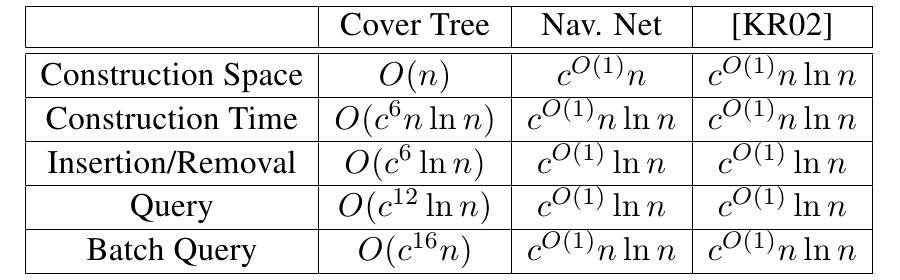
\includegraphics[width=12cm]{covertree/runtimes}

\begingroup
\begin{center}
\renewcommand*{\arraystretch}{1.9}
\begin{tabular}{l|c|c|}
& \footnotesize My Dissertation
& \footnotesize Beygelzimer \emph{et. al.}, 2006
\\
\hline
Number of nodes       & $n$                   & $O(n)$                \\
%Construction time     & $O(\cdoub^3n\log n$   & $O(\cexp^6 n\log n)$  \\
Insertion time (1 pt) & $O(\cdoub^3 \log n)$   & $O(\cexp^6 \log n)$   \\
Query time ~~~(1 pt)  & $O(\chole^4\log n)$    & $O(\cexp^{12}\log n)$ \\
%Query time ~~~(n pts) &  --                 & $\cexp^{16} n$     \\
\hline
\end{tabular}
\end{center}
\endgroup

\ignore{
{\footnotesize
    \begin{tabular}{>\centering m{2cm}|>\centering m{2.0cm}|>\centering m{2.0cm}|>\centering m{2.0cm}|c|}
    %\cline{2-5}
    & \multicolumn{2}{c|}{Cover Tree}
    %& Cover Tree
    & \footnotesize Nav. Net
    & \footnotesize Met. Skip List
    %& \footnotesize Ball Tree
    \\
    \cline{2-5}
    & \footnotesize My Dissertation
    & \footnotesize Beygelzimer ~~~\emph{et. al.}, 2006
    & \footnotesize Krauthgamer and Lee, 2004
    %& \footnotesize Karger and Ruhl, 2002
    & \begin{tabular}{c}
        Karger and\\
        Ruhl, 2002
      \end{tabular}
    %& \begin{tabular}{c}
        %Omohundro,\\
        %1989
      %\end{tabular}
    \\
    \hline
    Construction space    & $n$                 & $n$                & $\poly{\cexp}n$           & $\poly{\cexp}n \log n$    \\%& $n$ \\
    Construction time     & $\cdoub^3n\log n$   & $\cexp^6 n\log n$  & $\poly{\cexp}n\log n$     & $\poly{\cexp}n \log n$    \\%& $n^2$ \\
    Insertion time (1 pt) & $\cdoub^3 \log n$   & $\cexp^6 \log n$   & $\poly{\cexp}\log n$      & $\poly{\cexp} \log n$     \\%& $n$ \\
    Query time ~~~(1 pt)  & $\chole^4\log n$    & $\cexp^{12}\log n$ & $\poly{\cexp}\log n$      & $\poly{\cexp} \log n$     \\%& $n$\\
    Query time ~~~(n pts) &  --                 & $\cexp^{16} n$     & $\poly{\cexp}n\log n$     & $\poly{\cexp}n \log n$    \\%& $n^2$\\
    \hline

    \end{tabular}
}
}
%};

\vspace{0.15in}
The variables $\cdoub\approx\chole\approx\cexp$ measure the ``intrinsic dimension'' 

\vspace{0.15in}
%\footnotesize
%\node at (-1,-0.4) { (Beygelzimer \emph{et. al.}, 2006)};
%\node at (2,-1) { (Krauthgamer and Lee, 2004)};
%\node at (4,-0.4) { (Karger and Ruhl, 2002) };
%\draw[->] (-1,-0.25) -- (-0.9,0.1);
%\draw[->] (1.3,-0.75) -- (1.5,0.1);
%\end{tikzpicture}

%Karger and Ruhl, Symposium on the Theory of Computing, 2002
%
%\vspace{0.15in}
%Krauthgamer and Lee, Symposium on Discrete Algorithms, 2004
%
%\vspace{0.15in}
%Beygelzimer, Kakade, and Langford, ICML, 2006

\vspace{0.05in}
Recent research either:
\begin{itemize}
\item Extends the analysis on cover trees {\footnotesize (Ram \emph{et. al.}, 2010; Curtin \emph{et. al.}, 2015)}
\item Focuses on \emph{approximate} queries (too many papers to list)
\end{itemize}

%\vspace{0.15in}
%More recent research focuses on \emph{approximate} queries: LHS, Spill trees
%\textbf{open problem}: construct a data structure in time $O(c^{O(1)}n)$ for some dimensionality $c$; is it even possible?
%\vspace{0.15in}

\end{frame}


\newcommand\mybox[2][]{\tikz[overlay]\node[fill=lightyellow,inner sep=2pt, anchor=text, rectangle, rounded corners=1mm,draw=black,#1] {#2};\phantom{#2}}

\tikzstyle{reddot}=[draw=black,line width=1pt,minimum size=1.5mm,inner sep=0pt,outer sep=0pt,shape=circle,fill=blue]
\tikzstyle{bluedot}=[draw=blue,minimum size=0.5mm,inner sep=0pt,outer sep=0pt,shape=circle,fill=blue]

%%%%%%%%%%%%%%%%%%%%%%%%%%%%%%%%%%%%%%%%%%%%%%%%%%%%%%%%%%%%%%%%%%%%%%%%%%%%%%%%
\begin{frame}{The intrinsic dimension of data}

\begin{itemize}
\item
modern learning algorithms use high dimensional data

\item
\textbf{curse of dimensionality:}
\textcolor{red}{
the runtime of nearest neighbor queries grows exponentially with the dimension of data
}

\pause
\item
\textbf{manifold hypothesis:}
\textcolor{darkgreen}{
real world datasets are low dimensional manifolds embedded in high dimensional spaces
}
\end{itemize}

%Example:

\pause
\begin{center}
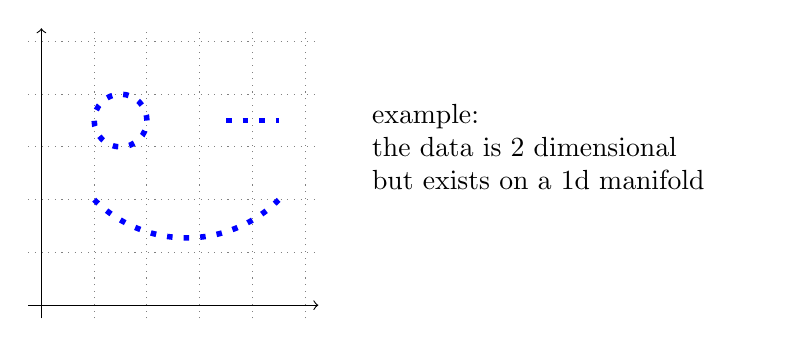
\begin{tikzpicture}[scale=0.67]
% draw the grid
\draw[->] (0,-0.25) -- (0,5.25) ;
\draw[->] (-0.25,0) -- (5.25,0) ;
\foreach \i in {1,...,5} {
    \draw[dotted,draw=gray] (-0.25,\i) -- (5.25,\i);
}
\foreach \i in {1,...,5} {
    \draw[dotted,draw=gray] (\i,-0.25) -- (\i,5.25);
}

\draw[loosely dotted,draw=blue,line width=2pt] (1,2) to[in=225,out=-45] (4.5,2);
\path[loosely dotted,draw=blue,line width=2pt] (1.5,3.5) circle (0.5);
\draw[loosely dotted,draw=blue,line width=2pt] (3.5,3.5) to (4.5,3.5);

\node[text width=5cm] at (10,3) {example: \\ the data is 2 dimensional \\ but exists on a 1d manifold};

\end{tikzpicture}
\end{center}

\end{frame}

%%%%%%%%%%%%%%%%%%%%%%%%%%%%%%%%%%%%%%%%%%%%%%%%%%%%%%%%%%%%%%%%%%%%%%%%%%%%%%%%

\begin{frame}{The intrinsic dimensions: \mybox{$\cexp$}, $\cdoub$, and $\chole$}

The \textbf{expansion constant} is defined as:
$$
\cexp = \max_{x\in X, \delta\ge0} \left\{
    \frac{|B(x,2\delta)|}{|B(x,\delta)|}
      \right\}
$$
\vspace{-0.1in}
where
$$
B(x,\delta) = \{x' \in X : d(x,x') \le \delta \}
$$
%is the ball of radius $\delta$ centered at point $x$.

\vspace{0.1in}
\hrule
\vspace{0.1in}
%%%%%%%%%%%%%%%%%%%%%%%%%%%%%%%%%%%%%%%%

\begin{tikzpicture}[scale=0.67]
% draw the grid
\draw[->] (0,-0.25) -- (0,5.25) ;
\draw[->] (-0.25,0) -- (5.25,0) ;
\foreach \i in {1,...,5} {
    \draw[dotted,draw=gray] (-0.25,\i) -- (5.25,\i);
}
\foreach \i in {1,...,5} {
    \draw[dotted,draw=gray] (\i,-0.25) -- (\i,5.25);
}

%\foreach \i in {1,...,10} {
    %\foreach \j in {1,...,10} {
        %\node[bluedot] at (0.3*\i,0.3*\j) {};
    %}
%}
\node[bluedot] at (2.5,2.5) {};
\foreach \i in {1,...,10} {
    \node[bluedot] at (2.5+0.2*\i,2.5-0.2*\i) {};
    \node[bluedot] at (2.5-0.2*\i,2.5+0.2*\i) {};
}

\uncover<2-5> {
\node[reddot] at (2.5,2.5) {};
\path[draw=black] (2.5,2.5) circle (1.4);
\path[draw=black] (2.5,2.5) circle (2.85);
}

\uncover<2-5> {
\node[fill=white] at (1.5,0) {\textcolor{darkgreen}{robust}};
\node at (2.5,-1) {\textcolor{darkgreen}{$\log\cexp=O(d)$}} ;
}
\end{tikzpicture}
%%%%%%%%%%%%%%%%%%%%
\begin{tikzpicture}[scale=0.67]
% draw the grid
\draw[->] (0,-0.25) -- (0,5.25) ;
\draw[->] (-0.25,0) -- (5.25,0) ;
\foreach \i in {1,...,5} {
    \draw[dotted,draw=gray] (-0.25,\i) -- (5.25,\i);
}
\foreach \i in {1,...,5} {
    \draw[dotted,draw=gray] (\i,-0.25) -- (\i,5.25);
}

\node[bluedot] at (2.5,2.5) {};
\foreach \i in {1,...,6} {
    \node[bluedot] at (3.3+0.2*\i,1.7-0.2*\i) {};
    \node[bluedot] at (1.7-0.2*\i,3.3+0.2*\i) {};
}

\uncover<3-5>{
\node[reddot] at (2.5,2.5) {};
\path[draw=black] (2.5,2.5) circle (1.4);
\path[draw=black] (2.5,2.5) circle (2.85);
}
\uncover<3-5> {
\node[fill=white] at (1.75,0) {\textcolor{red}{not robust}};
\node at (2.5,-1) {\textcolor{red}{$\cexp=O(n)$}} ;
}
\end{tikzpicture}
%%%%%%%%%%%%%%%%%%%%
\begin{tikzpicture}[scale=0.67]
% draw the grid
\draw[->] (0,-0.25) -- (0,5.25) ;
\draw[->] (-0.25,0) -- (5.25,0) ;
\foreach \i in {1,...,5} {
    \draw[dotted,draw=gray] (-0.25,\i) -- (5.25,\i);
}
\foreach \i in {1,...,5} {
    \draw[dotted,draw=gray] (\i,-0.25) -- (\i,5.25);
}

\node[bluedot] at (2.5,2.5) {};
\path[loosely dotted,draw=blue,line width=0.5mm] (2.5,2.5) circle (1.73);

\uncover<4-5>{
\node[reddot] at (2.5,2.5) {};
\path[draw=black] (2.5,2.5) circle (1.4);
\path[draw=black] (2.5,2.5) circle (2.85);
}
\uncover<4-5>   {
    \node[fill=white] at (1.75,0) {\textcolor{red}{not robust}};
    \node at (2.5,-1) {\textcolor{red}{$\cexp=O(n)$}};
}
\end{tikzpicture}

%%%%%%%%%%%%%%%%%%%%

\uncover<5>{
\vspace{-2.85in}
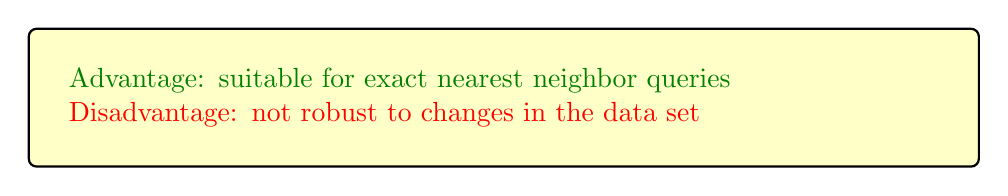
\begin{tikzpicture}
\node[fill=lightyellow,draw=black,thick,text width=11.05cm,rounded corners=0.1cm,inner sep=0.2in] at (0,0) { 
    \textcolor{darkgreen}{Advantage: suitable for exact nearest neighbor queries}
    \\
    \textcolor{red}{Disadvantage: not robust to changes in the data set}
    %\textcolor{red}{Disadvantage: cannot be used for exact nearest neighbor queries}
};
\end{tikzpicture}
}

\vspace{1.8in}

\end{frame}

%%%%%%%%%%%%%%%%%%%%%%%%%%%%%%%%%%%%%%%%%%%%%%%%%%%%%%%%%%%%%%%%%%%%%%%%%%%%%%%%

\begin{frame}{The intrinsic dimensions: $\cexp$, \mybox{$\cdoub$}, and $\chole$}

A set $C$ is a \textbf{$\delta$-covering} of $X$ if for all $x\in X$, there exists a $c \in C$ such that $\dist{x}{c} \le \delta$.
The \textbf{covering number} of $X$, denoted $N_\delta(X)$, is the cardinality of the smallest $\delta$-covering.
The \textbf{doubling constant} is 
\begin{equation}
\cdoub = \max_{x\in X,\delta>0} N_\delta( B(x,2\delta))
.
\end{equation}

%
%An \textbf{$r$-covering} of a set $X$ is a subset of $X$ such that all pairwise distances are greater than $r$. %$\{x_1,x_2,...x_M\} \subset X$ such that $\dist{x_i}{x_j} > r$ for all distinct $i,j$.
%
%The \textbf{$r$-packing number} $M_r (X)$ is the cardinality of the largest $r$-packing.
%

\vspace{0.1in}
\hrule
\vspace{0.1in}
%%%%%%%%%%%%%%%%%%%%%%%%%%%%%%%%%%%%%%%%

\begin{tikzpicture}[scale=0.67]
% draw the grid
\draw[->] (0,-0.25) -- (0,5.25) ;
\draw[->] (-0.25,0) -- (5.25,0) ;
\foreach \i in {1,...,5} {
    \draw[dotted,draw=gray] (-0.25,\i) -- (5.25,\i);
}
\foreach \i in {1,...,5} {
    \draw[dotted,draw=gray] (\i,-0.25) -- (\i,5.25);
}

%\foreach \i in {1,...,10} {
    %\foreach \j in {1,...,10} {
        %\node[bluedot] at (0.3*\i,0.3*\j) {};
    %}
%}
\node[bluedot] at (2.5,2.5) {};
\foreach \i in {1,...,10} {
    \node[bluedot] at (2.5+0.2*\i,2.5-0.2*\i) {};
    \node[bluedot] at (2.5-0.2*\i,2.5+0.2*\i) {};
}

\uncover<2-5> {
\node[reddot]  at (2.5,2.5) {};
\path[draw=black] (2.5,2.5) circle (1.4);
\path[draw=black] (2.5,2.5) circle (2.85);

\node[reddot]  at (1.3,3.7) {};
\path[draw=black] (1.3,3.7) circle (1.4);
\node[reddot]  at (3.7,1.3) {};
\path[draw=black] (3.7,1.3) circle (1.4);
}

\uncover<2-5> {
\node[fill=white] at (1.5,0) {\textcolor{darkgreen}{robust}};
\node at (2.5,-1) {\textcolor{darkgreen}{$\log\cdoub=O(d)$}} ;
}
\end{tikzpicture}
%%%%%%%%%%%%%%%%%%%%
\begin{tikzpicture}[scale=0.67]
% draw the grid
\draw[->] (0,-0.25) -- (0,5.25) ;
\draw[->] (-0.25,0) -- (5.25,0) ;
\foreach \i in {1,...,5} {
    \draw[dotted,draw=gray] (-0.25,\i) -- (5.25,\i);
}
\foreach \i in {1,...,5} {
    \draw[dotted,draw=gray] (\i,-0.25) -- (\i,5.25);
}

\node[bluedot] at (2.5,2.5) {};
\foreach \i in {1,...,6} {
    \node[bluedot] at (3.3+0.2*\i,1.7-0.2*\i) {};
    \node[bluedot] at (1.7-0.2*\i,3.3+0.2*\i) {};
}

\uncover<3-5>{
\node[reddot] at (2.5,2.5) {};
\path[draw=black] (2.5,2.5) circle (1.4);
\path[draw=black] (2.5,2.5) circle (2.85);

\node[reddot]  at (1.3,3.7) {};
\path[draw=black] (1.3,3.7) circle (1.4);
\node[reddot]  at (3.7,1.3) {};
\path[draw=black] (3.7,1.3) circle (1.4);
}
\uncover<3-5> {
\node[fill=white] at (1.5,0) {\textcolor{darkgreen}{robust}};
\node at (2.5,-1) {\textcolor{darkgreen}{$\log\cdoub=O(d)$}} ;
}
\end{tikzpicture}
%%%%%%%%%%%%%%%%%%%%
\begin{tikzpicture}[scale=0.67]
% draw the grid
\draw[->] (0,-0.25) -- (0,5.25) ;
\draw[->] (-0.25,0) -- (5.25,0) ;
\foreach \i in {1,...,5} {
    \draw[dotted,draw=gray] (-0.25,\i) -- (5.25,\i);
}
\foreach \i in {1,...,5} {
    \draw[dotted,draw=gray] (\i,-0.25) -- (\i,5.25);
}

\node[bluedot] at (2.5,2.5) {};
\path[loosely dotted,draw=blue,line width=0.5mm] (2.5,2.5) circle (1.73);

\uncover<4-5>{
\node[reddot] at (2.5,2.5) {};
\path[draw=black] (2.5,2.5) circle (1.4);
\path[draw=black] (2.5,2.5) circle (2.85);
}
\uncover<4-5>   {
\node[reddot]  at (1.3,3.7) {};
\path[draw=black] (1.3,3.7) circle (1.4);
\node[reddot]  at (3.7,3.7) {};
\path[draw=black] (3.7,3.7) circle (1.4);
\node[reddot]  at (3.7,1.3) {};
\path[draw=black] (3.7,1.3) circle (1.4);
\node[reddot]  at (1.3,1.3) {};
\path[draw=black] (1.3,1.3) circle (1.4);

    \node[fill=white] at (1.5,0) {\textcolor{darkgreen}{robust}};
    \node at (2.5,-1) {\textcolor{darkgreen}{$\log\cdoub=O(d)$}};
}
\end{tikzpicture}

\uncover<5>{
\vspace{-2.80in}
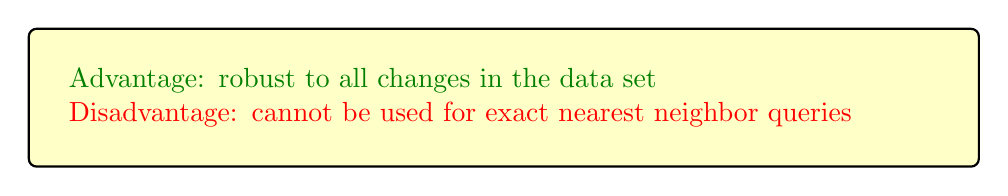
\begin{tikzpicture}
\node[fill=lightyellow,draw=black,thick,text width=11.05cm,rounded corners=0.1cm,inner sep=0.2in] at (0,0) { 
    \textcolor{darkgreen}{Advantage: robust to all changes in the data set}
    \\
    \textcolor{red}{Disadvantage: cannot be used for exact nearest neighbor queries}
};
\end{tikzpicture}
}

\vspace{1.8in}

\end{frame}

%%%%%%%%%%%%%%%%%%%%%%%%%%%%%%%%%%%%%%%%%%%%%%%%%%%%%%%%%%%%%%%%%%%%%%%%%%%%%%%%

\begin{frame}{The intrinsic dimensions: $\cexp$, $\cdoub$, and \mybox{$\chole$}}

%A set $C$ is a \textbf{$\delta$-covering} of $X$ if for all $x\in X$, there exists a $c \in C$ such that $\dist{x}{c} \le \delta$.
%The \textbf{covering number} of $X$, denoted $M_\delta(X)$, is the cardinality of the largest $\delta$-covering.
%The \textbf{doubling constant} is 
%\begin{equation}
%\cdoub = \max_{x\in X,\delta>0} M_\delta( B(x,2\delta))
%.
%\end{equation}
The \textbf{hole dimension} is like the doubling dimension,
but ignores a hole removed from the center of the enclosing ball.
It is defined as
\begin{align}
    \label{eq:chole}
    \chole
    = 
    &\max_{x\in X, \epsilon \ge 0, \delta > 0} 
    N_\delta\big( B(x,\epsilon+2\delta) \setminus B(x,\epsilon) \big)
    \\
    &
    ~~~~~~\text{s.t.}
    ~~
    %B(x,\epsilon+\delta) \setminus B(x,\delta) = \{\}
    B(x,\epsilon) = \{x\}
    .
\end{align}

%
%An \textbf{$r$-covering} of a set $X$ is a subset of $X$ such that all pairwise distances are greater than $r$. %$\{x_1,x_2,...x_M\} \subset X$ such that $\dist{x_i}{x_j} > r$ for all distinct $i,j$.
%
%The \textbf{$r$-packing number} $M_r (X)$ is the cardinality of the largest $r$-packing.
%

\vspace{0.1in}
\hrule
\vspace{0.1in}
%%%%%%%%%%%%%%%%%%%%%%%%%%%%%%%%%%%%%%%%

\begin{tikzpicture}[scale=0.67]
% draw the grid
\draw[->] (0,-0.25) -- (0,5.25) ;
\draw[->] (-0.25,0) -- (5.25,0) ;
\foreach \i in {1,...,5} {
    \draw[dotted,draw=gray] (-0.25,\i) -- (5.25,\i);
}
\foreach \i in {1,...,5} {
    \draw[dotted,draw=gray] (\i,-0.25) -- (\i,5.25);
}

%\foreach \i in {1,...,10} {
    %\foreach \j in {1,...,10} {
        %\node[bluedot] at (0.3*\i,0.3*\j) {};
    %}
%}
\node[bluedot] at (2.5,2.5) {};
\foreach \i in {1,...,9} {
    \node[bluedot] at (2.5+0.2*\i,2.5-0.2*\i) {};
    \node[bluedot] at (2.5-0.2*\i,2.5+0.2*\i) {};
}

\uncover<6-9> {
%\node[reddot]  at (2.5,2.5) {};
\path[draw=black] (2.5,2.5) circle (0.2);
\path[draw=black] (2.5,2.5) circle (2.6);

\path[draw=lightgray,opacity=0.5,line width=1.6cm] (2.5,2.5) circle (1.4);

\node[reddot]  at (1.5,3.5) {};
\path[draw=black] (1.5,3.5) circle (1.2);
\node[reddot]  at (3.5,1.5) {};
\path[draw=black] (3.5,1.5) circle (1.2);
}

\uncover<6-9> {
\node[fill=white] at (1.5,0) {\textcolor{darkgreen}{robust}};
\node at (2.5,-1) {\textcolor{darkgreen}{$\log\chole=O(d)$}} ;
}
\end{tikzpicture}
%%%%%%%%%%%%%%%%%%%%
\begin{tikzpicture}[scale=0.67]
% draw the grid
\draw[->] (0,-0.25) -- (0,5.25) ;
\draw[->] (-0.25,0) -- (5.25,0) ;
\foreach \i in {1,...,5} {
    \draw[dotted,draw=gray] (-0.25,\i) -- (5.25,\i);
}
\foreach \i in {1,...,5} {
    \draw[dotted,draw=gray] (\i,-0.25) -- (\i,5.25);
}

\node[bluedot] at (2.5,2.5) {};
\foreach \i in {1,...,5} {
    \node[bluedot] at (3.3+0.2*\i,1.7-0.2*\i) {};
    \node[bluedot] at (1.7-0.2*\i,3.3+0.2*\i) {};
}

\uncover<2-9> {
    \node[reddot]  at (2.5,2.5) {};
    \path[draw=black] (2.5,2.5) circle (1.35);
    \draw (2.5,2.5) -- node[above] {$\epsilon$} (3.85,2.5);
}
\uncover<3-9> {
    \path[draw=black] (2.5,2.5) circle (2.65);
    \path[draw=lightgray,opacity=0.5,line width=0.85cm] (2.5,2.5) circle (2);
    \draw (3.455,3.455) --  (4.365,4.365);
    \node at (3.75,4.25) {\small $2\delta$};
}
\uncover<4-9> {
    \node[reddot]  at (1.1,3.9) {};
    \path[draw=black] (1.1,3.9) circle (0.65);
    \node[reddot]  at (3.9,1.1) {};
    \path[draw=black] (3.9,1.1) circle (0.65);

    \draw(3.9,1.1) -- (4.4,1.6);
    \node at (4.0,1.5) {\small $\delta$};
}
\uncover<5-9> {
\node[fill=white] at (1.5,0) {\textcolor{darkgreen}{robust}};
\node at (2.5,-1) {\textcolor{darkgreen}{$\log\chole=O(d)$}} ;
}
\end{tikzpicture}
%%%%%%%%%%%%%%%%%%%%
\begin{tikzpicture}[scale=0.67]
% draw the grid
\draw[->] (0,-0.25) -- (0,5.25) ;
\draw[->] (-0.25,0) -- (5.25,0) ;
\foreach \i in {1,...,5} {
    \draw[dotted,draw=gray] (-0.25,\i) -- (5.25,\i);
}
\foreach \i in {1,...,5} {
    \draw[dotted,draw=gray] (\i,-0.25) -- (\i,5.25);
}

\node[bluedot] at (2.5,2.5) {};
\path[loosely dotted,draw=blue,line width=0.5mm] (2.5,2.5) circle (1.73);

\uncover<8-9>{
    \node[reddot] at (2.5,2.5) {};
    \path[draw=black] (2.5,2.5) circle (1.5);
    \path[draw=black] (2.5,2.5) circle (1.9);
    \path[draw=lightgray,opacity=0.5,line width=0.3cm] (2.5,2.5) circle (1.7);
}
    %\foreach \i in {1,...,20) {
        %\path[draw=black] (1.3*\i,1.3*\i) circle (0.2);
    %}
\uncover<8-9>   {
    \foreach \i in {10,...,47} {
        \path[draw=black] ({2.5+1.7*sin(\i/pi*29.2)} ,{2.5+1.7*cos(\i/pi*29.2)} ) circle (0.2);
        %\draw[dotted,draw=lightgray] (\i,-0.25) -- (\i,5.25);
    }
    %\path[draw=black] (1.3,3.7) circle (0.2);
    %\path[draw=black] (3.7,3.7) circle (0.2);
    %\path[draw=black] (3.7,1.3) circle (0.2);

    \node[fill=white] at (1.75,0) {\textcolor{red}{not robust}};
    \node at (2.5,-1) {\textcolor{red}{$\chole=O(n)$}};
}
\end{tikzpicture}

\uncover<9>{
\vspace{-2.85in}
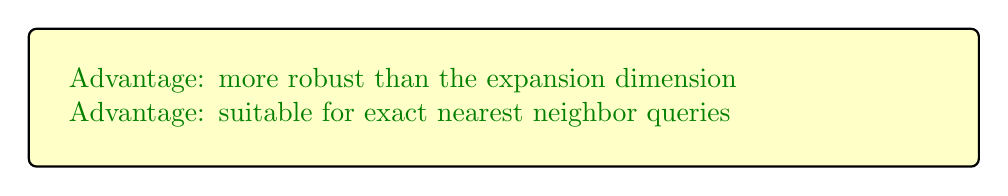
\begin{tikzpicture}
\node[fill=lightyellow,draw=black,thick,text width=11.05cm,rounded corners=0.1cm,inner sep=0.2in] at (0,0) { 
    \textcolor{darkgreen}{Advantage: more robust than the expansion dimension $\cexp$}
    \\
    \textcolor{darkgreen}{Advantage: suitable for exact nearest neighbor queries} 
    %\textcolor{red}{Disadvantage: cannot be used for exact nearest neighbor queries}
};
\end{tikzpicture}
}

\vspace{1.8in}

\end{frame}

%%%%%%%%%%%%%%%%%%%%%%%%%%%%%%%%%%%%%%%%%%%%%%%%%%%%%%%%%%%%%%%%%%%%%%%%%%%%%%%%

\begin{frame}{Experimental setup}
\Large

Three data sources:
\begin{itemize}
\item Protein dataset with the random walk graph distance
\item Yahoo! 1.5 million creative common images with the earth movers distance
\item MLPack benchmarks with Euclidean distance
    %\begin{itemize}
    %\item Selected the 8 largest datasets
    %\item Maximum size
    %\end{itemize}
\end{itemize}

\vspace{0.15in}
Benchmarking procedure:
\begin{itemize}
\item Construct a cover tree on the dataset
\item For each data point in the dataset, find the nearest neighbor
\item AWS instance with 16 true cores
\end{itemize}

\end{frame}

%%%%%%%%%%%%%%%%%%%%%%%%%%%%%%%%%%%%%%%%%%%%%%%%%%%%%%%%%%%%%%%%%%%%%%%%%%%%%%%%

\begin{frame}[fragile]{Experiment: protein data bank data}

%This experiment uses the protein data and the random walk graph kernel.
\vspace{0.1in}
Protein distance measured using the random walk graph kernel
\vspace{0.1in}

{
\begin{center}
\graphicspath{{slides/covertree/paperimg/}}
% GNUPLOT: LaTeX picture with Postscript
\begingroup
  \makeatletter
  \providecommand\color[2][]{%
    \GenericError{(gnuplot) \space\space\space\@spaces}{%
      Package color not loaded in conjunction with
      terminal option `colourtext'%
    }{See the gnuplot documentation for explanation.%
    }{Either use 'blacktext' in gnuplot or load the package
      color.sty in LaTeX.}%
    \renewcommand\color[2][]{}%
  }%
  \providecommand\includegraphics[2][]{%
    \GenericError{(gnuplot) \space\space\space\@spaces}{%
      Package graphicx or graphics not loaded%
    }{See the gnuplot documentation for explanation.%
    }{The gnuplot epslatex terminal needs graphicx.sty or graphics.sty.}%
    \renewcommand\includegraphics[2][]{}%
  }%
  \providecommand\rotatebox[2]{#2}%
  \@ifundefined{ifGPcolor}{%
    \newif\ifGPcolor
    \GPcolortrue
  }{}%
  \@ifundefined{ifGPblacktext}{%
    \newif\ifGPblacktext
    \GPblacktextfalse
  }{}%
  % define a \g@addto@macro without @ in the name:
  \let\gplgaddtomacro\g@addto@macro
  % define empty templates for all commands taking text:
  \gdef\gplbacktext{}%
  \gdef\gplfronttext{}%
  \makeatother
  \ifGPblacktext
    % no textcolor at all
    \def\colorrgb#1{}%
    \def\colorgray#1{}%
  \else
    % gray or color?
    \ifGPcolor
      \def\colorrgb#1{\color[rgb]{#1}}%
      \def\colorgray#1{\color[gray]{#1}}%
      \expandafter\def\csname LTw\endcsname{\color{white}}%
      \expandafter\def\csname LTb\endcsname{\color{black}}%
      \expandafter\def\csname LTa\endcsname{\color{black}}%
      \expandafter\def\csname LT0\endcsname{\color[rgb]{1,0,0}}%
      \expandafter\def\csname LT1\endcsname{\color[rgb]{0,1,0}}%
      \expandafter\def\csname LT2\endcsname{\color[rgb]{0,0,1}}%
      \expandafter\def\csname LT3\endcsname{\color[rgb]{1,0,1}}%
      \expandafter\def\csname LT4\endcsname{\color[rgb]{0,1,1}}%
      \expandafter\def\csname LT5\endcsname{\color[rgb]{1,1,0}}%
      \expandafter\def\csname LT6\endcsname{\color[rgb]{0,0,0}}%
      \expandafter\def\csname LT7\endcsname{\color[rgb]{1,0.3,0}}%
      \expandafter\def\csname LT8\endcsname{\color[rgb]{0.5,0.5,0.5}}%
    \else
      % gray
      \def\colorrgb#1{\color{black}}%
      \def\colorgray#1{\color[gray]{#1}}%
      \expandafter\def\csname LTw\endcsname{\color{white}}%
      \expandafter\def\csname LTb\endcsname{\color{black}}%
      \expandafter\def\csname LTa\endcsname{\color{black}}%
      \expandafter\def\csname LT0\endcsname{\color{black}}%
      \expandafter\def\csname LT1\endcsname{\color{black}}%
      \expandafter\def\csname LT2\endcsname{\color{black}}%
      \expandafter\def\csname LT3\endcsname{\color{black}}%
      \expandafter\def\csname LT4\endcsname{\color{black}}%
      \expandafter\def\csname LT5\endcsname{\color{black}}%
      \expandafter\def\csname LT6\endcsname{\color{black}}%
      \expandafter\def\csname LT7\endcsname{\color{black}}%
      \expandafter\def\csname LT8\endcsname{\color{black}}%
    \fi
  \fi
  \setlength{\unitlength}{0.0500bp}%
  \begin{picture}(5040.00,3772.00)%
    \gplgaddtomacro\gplbacktext{%
      \csname LTb\endcsname%
      \put(1298,704){\makebox(0,0)[r]{\strut{} 0}}%
      \put(1298,1054){\makebox(0,0)[r]{\strut{} 200}}%
      \put(1298,1405){\makebox(0,0)[r]{\strut{} 400}}%
      \put(1298,1755){\makebox(0,0)[r]{\strut{} 600}}%
      \put(1298,2106){\makebox(0,0)[r]{\strut{} 800}}%
      \put(1298,2456){\makebox(0,0)[r]{\strut{} 1000}}%
      \put(1298,2806){\makebox(0,0)[r]{\strut{} 1200}}%
      \put(1298,3157){\makebox(0,0)[r]{\strut{} 1400}}%
      \put(1298,3507){\makebox(0,0)[r]{\strut{} 1600}}%
      \put(1430,484){\makebox(0,0){\strut{} 0}}%
      \put(2073,484){\makebox(0,0){\strut{} 50}}%
      \put(2715,484){\makebox(0,0){\strut{} 100}}%
      \put(3358,484){\makebox(0,0){\strut{} 150}}%
      \put(4000,484){\makebox(0,0){\strut{} 200}}%
      \put(4643,484){\makebox(0,0){\strut{} 250}}%
      \put(176,2105){\rotatebox{-270}{\makebox(0,0){\strut{}total distance comparisons (millions)}}}%
      \put(396,2105){\rotatebox{-270}{\makebox(0,0){\strut{}on \emph{construction} and \emph{query}}}}%
      \put(3036,154){\makebox(0,0){\strut{}number of data points (thousands)}}%
    }%
    \gplgaddtomacro\gplfronttext{%
    }%
    \gplbacktext
    \put(0,0){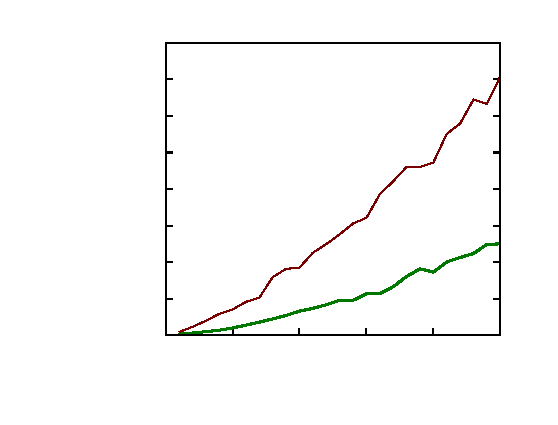
\includegraphics{protein-pres}}%
    \gplfronttext
  \end{picture}%
\endgroup

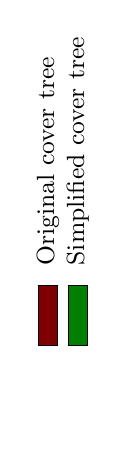
\begin{tikzpicture}
    \node[draw,fill=darkred,minimum width=0.03in,minimum height=0.3in] at (0,0) {};
    \node at (0,0.77in) {\small\rotatebox{90}{Original cover tree}};
    \node[draw,fill=darkgreen,minimum width=0.03in,minimum height=0.3in] at (0.15in,0) {};
    \node at (0.15in,0.82in) {\small\rotatebox{90}{Simplified cover tree}};
    %\node[draw,fill=blue,minimum width=0.03in,minimum height=0.3in] at (0.3in,0) {};
    %\node at (0.3in,1.01in) {\small\rotatebox{90}{Nearest ancestor cover tree}};
    %\node[minimum width=0.05in,minimum height=0.5in] at (0.45in,0) {};
    %\node at (0.6in,0.7in) {\small\rotatebox{90}{ dotted lines: construction only}};
    %\node at (0.75in,0.81in) {\small\rotatebox{90}{ solid lines: construction and query}};
    \node at (0,-0.5in) {};
\end{tikzpicture}
\end{center}
}

\end{frame}


\begin{frame}[fragile]{Experiment: Flickr image data}


%on small datasets with cheap metrics, parallel construction is less useful

%\vspace{0.1in}
%On large datasets with an expensive metric, parallelism is more useful

\vspace{0.15in}
Yahoo! Flickr dataset with 1.5 million images and earth mover distance

\vspace{0.15in}
Comparing the total runtime to construct the cover tree with parallelism

%\vspace{0.2in}
\vspace{0.15in}
\begin{center}
\Large
\begin{tabular}{ccc}
\hline
num cores
 %& \multicolumn{2}{c}{simplified cover tree} \\ %& \multicolumn{2}{c}{nearest ancestor tree} \\
%& \multicolumn{2}{c}{construction} & \multicolumn{2}{c}{construction} \\ %\cline{2-5}
& run time & speedup \\ %& time & speedup \\
\hline
\hline
1  & 70.7 min & 1.0 \\%& 210.9 min& 1.0\\
2  & 36.6 min & 1.9 \\%& 94.2 min & 2.2\\
4  & 18.5 min & 3.8 \\%& 48.5 min & 4.3\\
8  & 10.2 min & 6.9 \\%& 25.3 min & 8.3\\
16 & 6.7 min & 10.5 \\%& 12.0 min & 17.6\\
\hline
\end{tabular}
\end{center}

\end{frame}


\begin{frame}{Experiment: euclidean distance comparisons (1/4)}
\vspace{-0.25in}
\includegraphics[width=\textwidth]{img-website/mnist}
\end{frame}

\begin{frame}{Experiment: euclidean distance comparisons (2/4)}
\vspace{-0.25in}
\includegraphics[width=\textwidth]{img-website/tinyImages}
\end{frame}

\begin{frame}{Experiment: euclidean distance comparisons (3/4)}
\vspace{-0.25in}
\includegraphics[width=\textwidth]{img-website/twitter}
\end{frame}

\begin{frame}{Experiment: euclidean distance comparisons (4a/4)}
\vspace{-0.25in}
\includegraphics[width=\textwidth]{img-website/yearpredict}
\end{frame}

\begin{frame}{Experiment: euclidean distance comparisons (4b/4)}
\vspace{-0.25in}
\includegraphics[width=\textwidth]{img-website/yearpredict-parallel}
\end{frame}
%\includegraphics[width=.45\textwidth]{img-website/twitter}
%&
%\includegraphics[width=.45\textwidth]{img-website/yearpredict}


\begin{frame}{Other contributions}
\begin{itemize}
\item merge procedure for cover trees
\item the nearest ancestor invariant 
\item improved approximate nearest neighbor queries
\item improved cache efficiency
\end{itemize}
\end{frame}


\spacer{conclusion}
\begin{frame}{Summary of my dissertation}

\begin{itemize}
\item mergeable learning algorithms 
\begin{itemize}
    \item many examples in the literature
\item introduced a fast cross validation algorithm
\end{itemize}

\vspace{0.1in}
\item optimal weighted average (OWA)
\begin{itemize}
\item low variance and bias
\item easy to implement
\item computationally efficient
\end{itemize}

\vspace{0.1in}
\item faster cover tree
\begin{itemize}
\item improved theory
\begin{itemize}
\item the $\chole$ dimension for exact nearest neighbor queries
\item improve query runtime from $O(\cexp^{12}\log n)$ to $O(\chole^4\log n)$
\end{itemize}
\item improved practice
\begin{itemize}
\item simplified cover tree easier to implement and describe
%\item cache efficiency
\item merge procedure
\end{itemize}
\end{itemize}
\end{itemize}

\end{frame}

\begin{frame}{My publications}

%\fbox{\parbox{\textwidth}{Distributed Learning}}

    %\vspace{-0.3in}
%
    %~~~~~~~~~~~~~~~~~~~~~~~~~~~~~\colorbox{yellow}{\small (highlighted papers included in dissertation)}
%
    %\vspace{0.1in}
Faster machine learning 
\begin{itemize}
\item \hl{Algebraic classifiers (ICML 2013)}
\item \hl{Faster cover trees (ICML 2015)}
\item Identification of destabilizing attacks in power systems (ACC 2017)
\item \hl{Optimal distributed learning of linear models with limited}

      \hl{communication (under review)}
\end{itemize}

\vspace{0in}
Numeric programming in Haskell
\begin{itemize}
\item Many libraries for machine learning and numerical computation 

Not peer-reviewed: (TFP 2013, TMR 2013, MLOSS 2013, DCP 2014)\!\!\!\!\!\!
\end{itemize}


\vspace{0in}
Teaching 
\begin{itemize}
\item Mentored 6 undergrad open source projects
\item Developed curriculum for teaching open source 
    
    (ICOPUST 2015, 3rd place in research competition at SIGCSE 2016)
\item Lecturer for 7 classes at UCR and 4 classes at PUST (in DPRK)
\end{itemize}

\end{frame}

%{
%\usebackgroundtemplate{\includegraphics[width=\paperwidth]{img/pust-cs-marching2}}
%
%\begin{frame}{}
%%\uncover<2> {
%%\begin{tikzpicture}
%%\node at (0,3in) {};
%%\node[fill=white,draw=black] at (0,0) {\LARGE ICOPUST Machine Learning Workshop, Oct 2017};
%%\end{tikzpicture}
%%}
%\end{frame}
%}




\spacer{thank you! \\ \vspace{0.75in} questions?}

%%%%%%%%%%%%%%%%%%%%%%%%%%%%%%%%%%%%%%%%
\newcounter{finalframe}
\setcounter{finalframe}{\value{framenumber}}

\begin{frame}[fragile]{How should $\lambda$ be set?}

Local gridsearch over $\Lambda\subset\mathbb{R}$: 
\vspace{0.1in}

\noindent\fbox{%
%\begin{varwidth}{\dimexpr\linewidth-2\fboxsep-2\fboxrule\relax}
\begin{varwidth}{\linewidth}
\begin{algorithmic}
\State each machine $i$ in parallel:
\State ~~~~~\textbf{for} {$\lambda\in\Lambda$} \textbf{do}
    \State ~~~~~~~~~~calculates $\wmle_i(\lambda)$
    \State ~~~~~~~~~~evaluates $\wmle_i(\lambda)$ on local heldout set
    \State ~~~~~\textbf{end for}
    \State ~~~~~broadcasts locally optimal $\wmle_i$ to master
\State the master machine:
\State ~~~~~calculates and outputs $\wowa$ \hspace{2.45in}
    %\State ~~~~~evaluates $\wowa$ on a heldout validation set
%\State the master machine:
%\State ~~~~~outputs the $\wowa(\lambda)$ with lowest validation set error\hspace{1in}
\end{algorithmic}
\end{varwidth}%
}

\vspace{0.15in}
\textcolor{darkgreen}{one round of communication} ;
\textcolor{red}{greater bias due to incorrect $\lambda$}

\end{frame}

%%%%%%%%%%%%%%%%%%%%%%%%%%%%%%%%%%%%%%%%



\begin{frame}[fragile]{How should $\lambda$ be set? }

\textbf{Theory:}
Given $mn$ data points, the single machine ERM achieves optimal error rate with $\lambda=O(\sqrt{d/mn})$.

\vspace{0.15in}

\textbf{Experiment:}
Synthetic data drawn from a logistic regression model.

$m=20$, $mn=1000$, $d=100$; each trial repeated 100 times

\begin{center}
%\pgfplotsset{width=4in, height=2.3in, scale only axis}
\newcommand{\mklambdaplot}[3]{
\begin{tikzpicture}
    [ yscale=0.8
    ]
#3
\begin{axis}
    [ width=4in
    , height=2.3in
    , xmode=log
    , ymode=log
    , xmin=10^-4
    , xmax=10^4
    , xtick={0.0001,0.01,1,100,10000}
    , xticklabels={$10^{4}$,$10^{2}$,$10^{0}$,$10^{-2}$,$10^{-4}$}
    , enlarge y limits=0
    , x dir=reverse
#2
    ]
%\addplot[black,no marks] table [x index=3,y index=5] {#1};
\addplot[wmlei,no marks,thick] table [x index=3,y index=7] {#1};
\addplot[wave,no marks] table [x index=3,y index=9] {#1};
%\addplot[red,thick,no marks] table [x index=3,y index=17] {#1};
\only<2-3>{\addplot[wowa,very thick,no marks] table [x index=3,y index=55] {#1};}
%\addplot[dotted,wowa,very thick,no marks] table [x index=3,y index=56] {#1};
%\addplot[wowa,thin,no marks] table [x index=3,y index=56] {#1};
%\addplot[thick,red,no marks] table [x=n,y=bootll] {dat/kdd-scaling.dat};
%\addplot[very thick,wowa,no marks] table [x=n,y=owall] {dat/kdd-scaling.dat};
\end{axis}
%\node at (2.2,-0.8) {\small regularization strength ($\lambda$)};

%\draw[wmlei, line width=1.5pt] (5.05,0) -- (5.05,4.25);
%\draw[wave, line width=1.5pt] (4.8,0) -- (4.8,4.25);

\end{tikzpicture}
}
\begin{tabular}{cc}
{\small\rotatebox{90}{\hspace{1.0cm}error $\ltwo{\wstar-\w}$}}
&\hspace{-0.5cm}\mklambdaplot
    {dat.rev/logl1-star-logl2-autoreg-spike-log-1000-100-20.pdf.csv}
    {,ymin=10^-2,ymax=10^2,ytick={0.01,0.1,1,10,100}}{
    \node at (2,3.1) {\textcolor{wmlei}{$\wmle_i$}};
    \draw[->,wmlei] (2,3.0) -- (2.1,2.7);
    \node at (3.5,1.5) {\textcolor{wave}{$\wave$}};
    \draw[->,wave] (3.1,1.5) -- (3.0,1.85);
    %\node at (4,1.1) {\textcolor{red}{$\wboot$}};
    %\draw[->,thick,red] (3.8,1.3) -- (3.75,1.45);
    %\node at (7.7,1.95) {$\wmle$};
    %\draw[->] (7.2,1.9) -- (6.9,1.9);
    \uncover<2-3>{\node at (7,0.9) {\textcolor{wowa}{$\wowa$}};
    \draw[->,thick,wowa] (6.5,0.8) -- (6.2,0.8);}
    %\node at (0.6,0.4) {\textcolor{wowa}{$\wowafull$}};
    %\draw[->,thick,dotted,wowa] (0.9,0.3) -- (1.2,0.3);
    %\draw[->,very thin,wowa] (0.9,0.3) -- (1.2,0.3);

    \uncover<3>{\node at (7.5,1.5) {\textcolor{wowa}{why?}};}
    }
%&\hspace{-0.5cm}\mklambdaplot
    %{dat/logl1-star-logl2-auto-spike-log-1000-100-100.pdf.csv}
    %{,ymin=10^-3,ymax=10^2,ytick={0.001,0.01,0.1,1,10,100}}
    %{}
%&\hspace{-0.5cm}\mklambdaplot
    %{dat/logl1-star-logl2-auto-spike-log-1000-1000-100.pdf.csv}
    %{,ymin=10^-1,ymax=10^3,ytick={0.1,1,10,100,1000}}
    %{}
\\
& \hspace{0.2cm} {\small regularization strength ($\lambda$)}
\end{tabular}
\end{center}

\end{frame}




%%%%%%%%%%%%%%%%%%%%%%%%%%%%%%%%%%%%%%%%

\begin{frame}{Efficiently calculating $\wowa$}

%Let $\matW = \bigg(\wmle_1, \wmle_2, ..., \wmle_m\bigg) \in \mathbb R^{d\times m}$
%
%\vspace{0.1in}
%Then every $\w\in\Wowa$ can be written as $\w=\matW\alpha$, where $\alpha\in\mathbb R^m$

\vspace{0.1in}
We can rewrite $\wowa$ as
%$\wowa = \matW \ahat$
%where
\begin{align}
\wowa &= \matW \ahat
\\
\label{eq:afull}
\ahat &= \argmax_{\alpha\in\mathbb R^m} \sum _{(\x,y)\in \Zowa} \loss\left(y,\trans\x \matW \alpha \right)
+
\lambda \reg(\matW\alpha)
\\
\matW &= \bigg(\wmle_1, \wmle_2, ..., \wmle_m\bigg) \in \mathbb R^{d\times m}
\end{align}

%In the second round of communication
%\begin{itemize}
%\item Each machine transmits $\trans\x\matW$ for each data point in $\Zowa$
%\item This is $O(m)$ bits per data point 
%
%~~~~~~~~~$O(m\nowa)$ bits per machine
%
%~~~~~~~~~$O(m^2\nowa)$ bits total
%%\item Whenever $m\nowa < d$, fewer bits are transfered than the first round
%\end{itemize}

\pause
Notice that:
\begin{itemize}
%\item
%The merging procedure depends on the data,
%so existing impossibility theorems do not apply.

%\pause
\item
The $\ahat$ optimization happens in a low dimensional subspace, so few datapoints are needed.

\pause
\item
The $\trans\x\matW$ in $(11)$ does not depend on $\alpha$, so needs to be computed only once (instead of each iteration).

%\pause
%\item
%The $\Zowa$ dataset should be stored already on the reduce server.
%
%(In the paper, we provide an algorithm for efficiently communicating the $\Zowa$ dataset to the reducer if needed.)

\end{itemize}

\end{frame}




\newtheorem{defn}{Definition}
\begin{frame}[fragile]{Metric spaces generalize euclidean space}
\centering
\resizebox{!}{4.5cm}{
\begin{tikzpicture}[dot/.style={circle,inner sep=2pt,fill,name=#1},
    extended line/.style={shorten >=-#1,shorten <=-#1},
    extended line/.default=1cm]

% draw the grid
\uncover<1-3> {
    \draw[->] (0,-0.25) -- (0,5.25) ;
    \draw[->] (-0.25,0) -- (5.25,0) ;
    \foreach \i in {1,...,5} {
        \draw[dotted] (-0.25,\i) -- (5.25,\i);
        \draw[dotted] (\i,-0.25) -- (\i,5.25);
    }
}

% draw the points
\uncover<1-3> {
    \node [dot=a,label=above left:a] at (1,1) {};
    \node [dot=b,label=above:b] at (2,4) {};
    \node [dot=c,label=above right:c] at (4,2) {};
}

% draw the L2 metric
\uncover<1> {
    \draw (a) -- (b) -- (c) -- (a);
    \node at (3,1.25) {$\sqrt{10}$};
    \node at (1,2.75) {$\sqrt{10}$};
    \node at (3.5,3.25) {$2\sqrt{2}$};
    \node at (8, 4.5) {
        Euclidean distance:
        };
    \node at (9,2.5) {

        $\begin{aligned}
        \mathcal{X}& = \mathbb{R}^p \\
        \displaystyle
        d(x,y)
        &=
        \displaystyle
        \left(\sum_{i=1}^p (x_i-y_i)^2\right)^{\frac 1 2} \\
        \end{aligned}$
        };
    \node at (9, 0.5) { Runtime to calculate distance: $O(p)$ };
}

% draw the L1 metric
\uncover<2> {
    \draw (a) -- (1,4) -- (b) -- (4,4) -- (c) -- (4,1) -- (a);
    \node at (2.5,1.25) {$4$};
    \node at (1.25,2.75) {$4$};
    \node at (3.5,3.5) {$4$};
    \node at (9, 4.5) {
        $L_1$ (Manhattan, taxicab) distance:
        };
    \node at (9,2.5) {
        $\begin{aligned}
        \mathcal{X}& = \mathbb{R}^p \\
        \displaystyle
        d(x,y)
        &=
        \displaystyle
        \sum_{i=1}^p |x_i-y_i| \\
        \end{aligned}$
        };
    \node at (9, 0.5) { Runtime to calculate distance: $O(p)$ };
}

% draw the Linf metric
\uncover<3> {
    \draw (a) -- (1,4);
    \draw (4,4) -- (c);
    \draw (a) -- (4,1);
    \node at (2.5,1.25) {$3$};
    \node at (1.25,2.75) {$3$};
    \node at (3.5,3.5) {$2$};
    \node at (8, 4.5) {
        $L_\infty$ (sup) distance:
        };
    \node at (9,2.5) {
        $\begin{aligned}
        \mathcal{X}& = \mathbb{R}^p \\
        \displaystyle
        d(x,y)
        &=
        \displaystyle
        \sup_{i\in\{1..p\}} |x_i-y_i| \\
        \end{aligned}$
        };
    \node at (9, 0.5) { Runtime to calculate distance: $O(p)$ };
}

%% draw the Lebesgue metric
%\uncover<4> {
    %\node at (9, 4.5) {
        %Lebesgue family of distances:
        %};
    %\node at (9,2.5) {
        %$\begin{aligned}
        %\mathcal{X}& = \mathbb{R}^n \\
        %\displaystyle
        %d(x,y)
        %&=
        %\displaystyle
        %\left(\sum_{i\in\{1..n\}} |x_i-y_i|^n\right)^{\frac 1 n} \\
        %\end{aligned}$
        %};
    %\node at (9, 0.5) { Runtime to calculate distance: $O(n)$ };
%}

%% graph distances
%\uncover <6-7> {
    %\draw[color=red,line width=2pt] (3.35,3.1) -- (3.65,3.4);
    %\node[color=red] at (4,3.25) {\textbf{1?}};
%}
%\uncover<6> {
    %\draw[color=red,line width=2pt] (6,0) -- (12,5);
%}

%\uncover<5-6> {
    %\draw (a) -- (b) -- (c) -- (a);
    %\node at (3,1.25) {$2$};
    %\node at (1,2.75) {$4$};
    %\node at (3.5,3.25) {$5$};
    %\node at (9, 4.5) {
        %weighted, fully-connected graph distance
        %};
    %\node at (9,2.5) {
        %$\begin{aligned}
        %\mathcal{X}& = \{a,b,c\} \\
        %\displaystyle
        %d(x,y)
        %&=
        %\text{edge weight}
        %\end{aligned}$
        %};
    %\node at (9, 0.5) { Runtime to calculate distance: $O(1)$ };
%}

%% graph distances
%\uncover<7> {
    %\draw (a) -- (b) -- (c) -- (a);
    %\node at (3,1.25) {$2$};
    %\node at (1,2.75) {$4$};
    %\node at (3.5,3.25) {$5$};
    %\node at (9, 4.5) {
        %Dijkstra graph distance
        %};
    %\node at (9,2.5) {
        %$\begin{aligned}
        %\mathcal{X}& = \{a,b,c\} \\
        %\displaystyle
        %d(x,y)
        %&=
        %\text{shortest path between $x$ and $y$}
        %\end{aligned}$
        %};
    %\node at (9, 0.5) { Runtime to calculate distance: $O(e+v\log v)$ };
%}

%% graph distances
%\uncover<8> {
    %\draw (a) -- (b);
    %\draw (c) -- (a);
    %\node at (3,1.25) {$2$};
    %\node at (1,2.75) {$4$};
    %\node at (9, 4.5) {
        %Dijkstra graph distance
        %};
    %\node at (9,2.5) {
        %$\begin{aligned}
        %\mathcal{X}& = \{a,b,c\} \\
        %\displaystyle
        %d(x,y)
        %&=
        %\text{shortest path between $x$ and $y$}
        %\end{aligned}$
        %};
    %\node at (9, 0.5) { Runtime to calculate distance: $O(e+v\log v)$ };
%}

%% graph distances
%\uncover<9> {
    %\draw (a) -- (b);
    %\node at (1,2.75) {$4$};
    %\node at (9, 4.5) {
        %Dijkstra graph distance
        %};
    %\node at (9,2.5) {
        %$\begin{aligned}
        %\mathcal{X}& = \{a,b,c\} \\
        %\displaystyle
        %d(x,y)
        %&=
        %\text{shortest path between $x$ and $y$}
        %\end{aligned}$
        %};
    %\node at (9, 0.5) { Runtime to calculate distance: $O(e+v\log v)$ };
%}

%% graph distances
%\uncover<10> {
    %\node at (8, 4.5) {
        %trivial distance
        %};
    %\node at (9,2.5) {
        %$\begin{aligned}
        %\mathcal{X}& = \{a,b,c\} \\
        %\displaystyle
        %d(x,y)
        %&=
        %\infty
        %\end{aligned}$
        %};
    %\node at (9, 0.5) { Runtime to calculate distance: $O(1)$ };
%}

%% graph distances
%\uncover<11> {
    %\node at (1,3) {
        %$d \left(
        %\text{
        %\begin{tikzpicture}
        %\node at (0,2) {};
        %\node [dot= ] at (1,1) {};
        %\node [dot= ] at (1,0) {};
        %\node [dot= ] at (0,1) {};
        %\draw (1,1) -- (1,0) -- (0,1) -- (1,1);
        %\end{tikzpicture}
        %,
        %\begin{tikzpicture}
        %\node at (0,2) {};
        %\node [dot= ] at (1,1) {};
        %\node [dot= ] at (1,0) {};
        %\node [dot= ] at (0,1) {};
        %\node [dot= ] at (0,0) {};
        %\draw (1,1) -- (1,0) -- (0,1) -- (1,1) -- (0,0) -- (0,1) -- (1,0) -- (0,0);
        %\end{tikzpicture}
        %}
        %\right)$
    %};
    %\node at (9, 4.5) {
        %\emph{graph metrics} are distances between graphs
        %};
    %\node at (9,2.5) {
        %$\begin{aligned}
        %\mathcal{X}& = \text{set of all graphs} \\
        %\displaystyle
        %d(x,y)
        %&=
        %\text{many possibilities}
        %\end{aligned}$
        %};
    %\node at (9, 0.5) { Runtime to calculate distance: $O(1)$ };
%}

\end{tikzpicture}
}
\begin{defn}
A \emph{metric space} is a set $\mathcal{X}$ equiped with a distance function $d : \mathcal{X} \times \mathcal{X} \rightarrow \mathbb{R}$ such that:
\begin{center}
\begin{tabular}{ll}
$d(x,y) \ge 0$ & $d(x,y) = 0$ iff $x=y$ \\
$d(x,y) = d(y,x)$ & $d(x,z) \le d(x,y) + d(y,z)$ \\
\end{tabular}
\end{center}
\end{defn}
\end{frame}



\begin{frame}[fragile]{Metrics for proteins}

\vspace{-0.3in}
\begin{center}
\begin{tikzpicture}
%\node at (0,0) {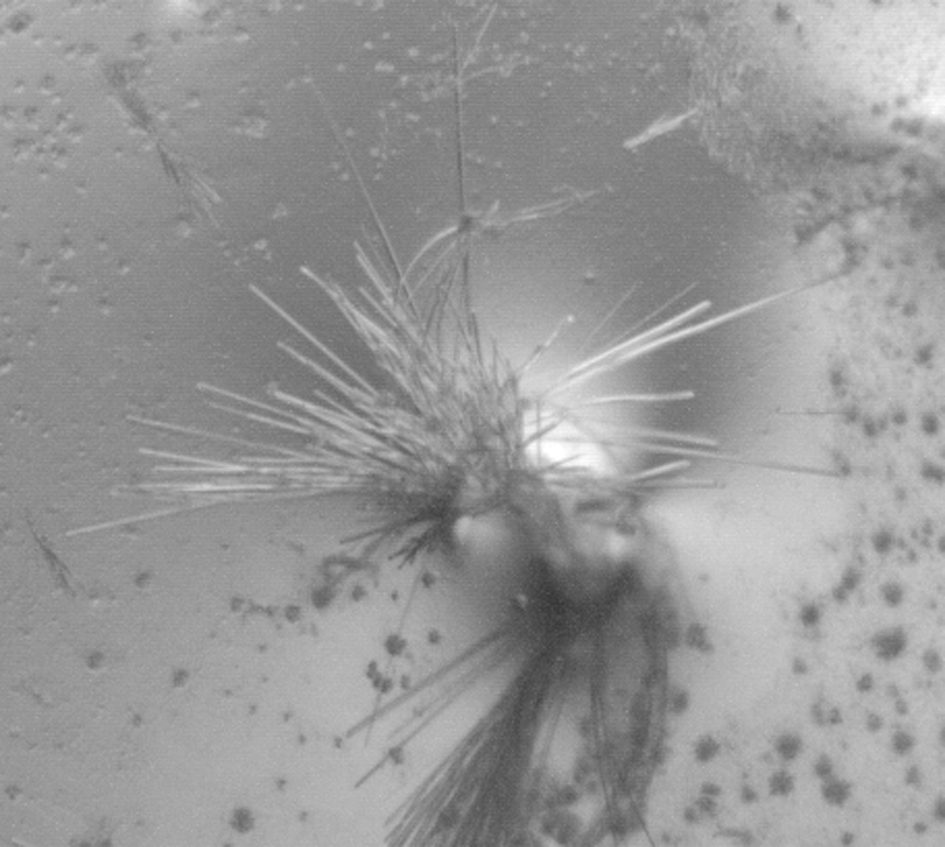
\includegraphics[width=4cm]{slides/covertree/xrayprotein}};
\node at (0,0) {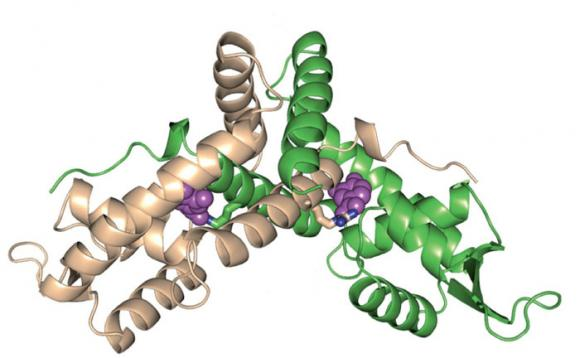
\includegraphics[width=4cm]{img-presentation/Lignin1_0}};
\node at (6,0) {\includegraphics[width=4cm]{slides/covertree/ProteinGraphs}};

\draw[->,line width=4pt] (2.75,0) -- (3.75,0);
\end{tikzpicture}
\end{center}

\vspace{-0.2in}

%The protein databank contains information on $\sim$100,000 proteins
%
%\vspace{0.1in}
Protein structure (and hence function) can be modeled as a graph

\vspace{0.1in}
The random walk graph kernel is a commonly used protein metric

\vspace{0.1in}
This is an \emph{expensive} metric, taking time $O(v^3)$

\vspace{0.1in}
(Vishwanathan \emph{et. al.}, 2010)

\vspace{0.15in}
{\tiny
images from: \url{http://www.lunenfeld.ca}, and \url{http://vishgraph.mbu.iisc.ernet.in/GraProStr/}
}

\end{frame}



\begin{frame}[fragile]{Metrics for images}
\includegraphics[width=6cm]{slides/covertree/imagehistogram2.png}
\includegraphics[width=6cm]{slides/covertree/imagehistogram3b.jpg}

\vspace{0.15in}
There are \emph{lots} of distance metrics for images.
Histogram metrics follow the two step process:
\begin{itemize}
\item generate histograms (usually of colors)
\item define a distance between histograms
\end{itemize}

Earth mover's distance is a popular but slow metric.
It runs in time $O(b^3 \log b)$, where $b$ is the size of the histogram.
(Rubner \emph{et. al.}, 1998)

\vspace{0.05in}
{\tiny
images from: \url{http://billmill.org/the_histogram.html}
}
\end{frame}


%\begin{frame}[fragile]{metrics for images}
%\includegraphics[width=12cm]{slides/covertree/emd.png}
%
%\end{frame}

\begin{frame}[fragile]{The simplified cover tree}

\begin{center}
\begin{tikzpicture}
    [ draw
    , every node/.style={minimum size=10mm,fill=white}
    , level/.style={sibling distance = 23mm/#1, level distance=12mm}
    %,    level distance = 1.5cm}
    , sibling distance=8mm
    ]
\draw (-2.3,0) -- (8.6,0)[dotted];
\draw (-2.3,-12mm) -- (8.6,-12mm)[dotted];
\draw (-2.3,-24mm) -- (8.6,-24mm)[dotted];
\node[shape=circle,draw] at (2.5,0) {10}
    child { node[circle,draw] {8}
        child { node[circle,draw] {7}  }
        child { node[circle,draw] {9} }
        }
    child { node[circle,draw] {12}
        %child { node[circle,draw,fill=lightred,line width=1pt] {9}  }
        %child { node[circle,draw] {13} }
        }
    ;
%\node[shape=circle,draw] at (5,0) {10}
    %child { node[circle,draw] {8}
        %child { node[circle,draw] {7}  }
        %child { node[circle,draw,fill=lightgreen,line width=1pt] {9} }
        %}
    %child { node[circle,draw] {12}
        %child { node[circle,draw,fill=lightgreen,line width=1pt] {11}  }
        %child { node[circle,draw] {13} }
        %}
    %;
\node[fill=none] at (8,3mm) {level 3};
\node[fill=none] at (8,-9mm) {level 2};
\node[fill=none] at (8,-21mm) {level 1};
\end{tikzpicture}
\end{center}

\uncover<1> {
%\vspace{0.15in}
\textbf{The covering invariant.}
For every node $p$, define the function $\covdist p = \exprad p^{\level p}$.
For each child $q$ of $p$
$$
\dist p q \le \covdist p
$$

\vspace{0.15in}
\textbf{The separating invariant.}
For every node $p$, define the function $\sepdist p = \exprad p^{\level p-1}$.
For all distinct children $q_1$ and $q_2$ of $p$
$$
\dist{q_1}{q_2} \ge \sepdist p
$$
}

\uncover<2> {
\vspace{-1.70in}
Advantages of the simplified cover tree:
\vspace{0.05in}
\begin{itemize}
\item Maintains all runtime guarantees of the original cover tree.
\vspace{0.05in}

\item Significantly easier to understand and implement.

%\vspace{0.05in}
The original cover tree was described in terms of an infinitely large tree, only a subset of which actually gets implemented.

\vspace{0.05in}
\item Requires exactly $n$ nodes instead of $O(n)$ nodes.

%\vspace{0.05in}
Fewer nodes means a faster constant factor for all algorithms. %insertions and queries are faster.
\end{itemize}
\vspace{1.3in}
}

\end{frame}


\begin{frame}[fragile]{The simplified cover tree}

\centering
\graphicspath{{slides/covertree/paperimg/}}
% GNUPLOT: LaTeX picture with Postscript
\begingroup
  \makeatletter
  \providecommand\color[2][]{%
    \GenericError{(gnuplot) \space\space\space\@spaces}{%
      Package color not loaded in conjunction with
      terminal option `colourtext'%
    }{See the gnuplot documentation for explanation.%
    }{Either use 'blacktext' in gnuplot or load the package
      color.sty in LaTeX.}%
    \renewcommand\color[2][]{}%
  }%
  \providecommand\includegraphics[2][]{%
    \GenericError{(gnuplot) \space\space\space\@spaces}{%
      Package graphicx or graphics not loaded%
    }{See the gnuplot documentation for explanation.%
    }{The gnuplot epslatex terminal needs graphicx.sty or graphics.sty.}%
    \renewcommand\includegraphics[2][]{}%
  }%
  \providecommand\rotatebox[2]{#2}%
  \@ifundefined{ifGPcolor}{%
    \newif\ifGPcolor
    \GPcolortrue
  }{}%
  \@ifundefined{ifGPblacktext}{%
    \newif\ifGPblacktext
    \GPblacktextfalse
  }{}%
  % define a \g@addto@macro without @ in the name:
  \let\gplgaddtomacro\g@addto@macro
  % define empty templates for all commands taking text:
  \gdef\gplbacktext{}%
  \gdef\gplfronttext{}%
  \makeatother
  \ifGPblacktext
    % no textcolor at all
    \def\colorrgb#1{}%
    \def\colorgray#1{}%
  \else
    % gray or color?
    \ifGPcolor
      \def\colorrgb#1{\color[rgb]{#1}}%
      \def\colorgray#1{\color[gray]{#1}}%
      \expandafter\def\csname LTw\endcsname{\color{white}}%
      \expandafter\def\csname LTb\endcsname{\color{black}}%
      \expandafter\def\csname LTa\endcsname{\color{black}}%
      \expandafter\def\csname LT0\endcsname{\color[rgb]{1,0,0}}%
      \expandafter\def\csname LT1\endcsname{\color[rgb]{0,1,0}}%
      \expandafter\def\csname LT2\endcsname{\color[rgb]{0,0,1}}%
      \expandafter\def\csname LT3\endcsname{\color[rgb]{1,0,1}}%
      \expandafter\def\csname LT4\endcsname{\color[rgb]{0,1,1}}%
      \expandafter\def\csname LT5\endcsname{\color[rgb]{1,1,0}}%
      \expandafter\def\csname LT6\endcsname{\color[rgb]{0,0,0}}%
      \expandafter\def\csname LT7\endcsname{\color[rgb]{1,0.3,0}}%
      \expandafter\def\csname LT8\endcsname{\color[rgb]{0.5,0.5,0.5}}%
    \else
      % gray
      \def\colorrgb#1{\color{black}}%
      \def\colorgray#1{\color[gray]{#1}}%
      \expandafter\def\csname LTw\endcsname{\color{white}}%
      \expandafter\def\csname LTb\endcsname{\color{black}}%
      \expandafter\def\csname LTa\endcsname{\color{black}}%
      \expandafter\def\csname LT0\endcsname{\color{black}}%
      \expandafter\def\csname LT1\endcsname{\color{black}}%
      \expandafter\def\csname LT2\endcsname{\color{black}}%
      \expandafter\def\csname LT3\endcsname{\color{black}}%
      \expandafter\def\csname LT4\endcsname{\color{black}}%
      \expandafter\def\csname LT5\endcsname{\color{black}}%
      \expandafter\def\csname LT6\endcsname{\color{black}}%
      \expandafter\def\csname LT7\endcsname{\color{black}}%
      \expandafter\def\csname LT8\endcsname{\color{black}}%
    \fi
  \fi
  \setlength{\unitlength}{0.0500bp}%
  \begin{picture}(5040.00,3772.00)%
    \gplgaddtomacro\gplbacktext{%
      \csname LTb\endcsname%
      \put(1166,780){\makebox(0,0)[r]{\strut{} 0}}%
      \put(1166,1053){\makebox(0,0)[r]{\strut{} 0.1}}%
      \put(1166,1325){\makebox(0,0)[r]{\strut{} 0.2}}%
      \put(1166,1598){\makebox(0,0)[r]{\strut{} 0.3}}%
      \put(1166,1871){\makebox(0,0)[r]{\strut{} 0.4}}%
      \put(1166,2144){\makebox(0,0)[r]{\strut{} 0.5}}%
      \put(1166,2416){\makebox(0,0)[r]{\strut{} 0.6}}%
      \put(1166,2689){\makebox(0,0)[r]{\strut{} 0.7}}%
      \put(1166,2962){\makebox(0,0)[r]{\strut{} 0.8}}%
      \put(1166,3234){\makebox(0,0)[r]{\strut{} 0.9}}%
      \put(1166,3507){\makebox(0,0)[r]{\strut{} 1}}%
      \put(1661,648){\rotatebox{-45}{\makebox(0,0)[l]{\strut{}yearpredict}}}%
      \put(2023,648){\rotatebox{-45}{\makebox(0,0)[l]{\strut{}twitter}}}%
      \put(2386,648){\rotatebox{-45}{\makebox(0,0)[l]{\strut{}tinyImages}}}%
      \put(2748,648){\rotatebox{-45}{\makebox(0,0)[l]{\strut{}mnist}}}%
      \put(3111,648){\rotatebox{-45}{\makebox(0,0)[l]{\strut{}corel}}}%
      \put(3473,648){\rotatebox{-45}{\makebox(0,0)[l]{\strut{}covtype}}}%
      \put(3836,648){\rotatebox{-45}{\makebox(0,0)[l]{\strut{}artificial40}}}%
      \put(4198,648){\rotatebox{-45}{\makebox(0,0)[l]{\strut{}faces}}}%
      \put(176,2143){\rotatebox{-270}{\makebox(0,0){\strut{}fraction of nodes in the original cover tree }}}%
      \put(396,2143){\rotatebox{-270}{\makebox(0,0){\strut{} required for the simplified cover tree}}}%
    }%
    \gplgaddtomacro\gplfronttext{%
    }%
    \gplbacktext
    \put(0,0){\includegraphics{nodes}}%
    \gplfronttext
  \end{picture}%
\endgroup


\end{frame}

\begin{frame}[fragile]{The nearest ancestor cover tree}

\definecolor{lightred}{rgb}{1,0.8,0.8}
\definecolor{lightgreen}{rgb}{0.8,1,0.8}
\begin{center}
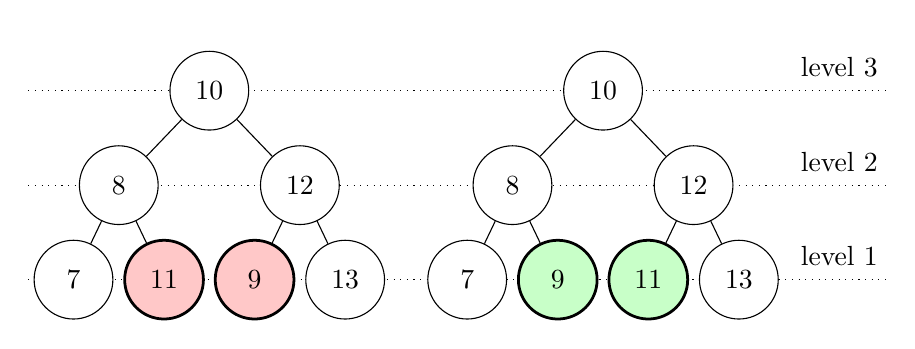
\begin{tikzpicture}
    [ draw
    , every node/.style={minimum size=10mm,fill=white}
    , level/.style={sibling distance = 23mm/#1, level distance=12mm}
    %,    level distance = 1.5cm}
    , sibling distance=8mm
    ]
\draw (-2.3,0) -- (8.6,0)[dotted];
\draw (-2.3,-12mm) -- (8.6,-12mm)[dotted];
\draw (-2.3,-24mm) -- (8.6,-24mm)[dotted];
\node[shape=circle,draw] at (0,0) {10}
    child { node[circle,draw] {8}
        child { node[circle,draw] {7}  }
        child { node[circle,draw,fill=lightred,line width=1pt] {11} }
        }
    child { node[circle,draw] {12}
        child { node[circle,draw,fill=lightred,line width=1pt] {9}  }
        child { node[circle,draw] {13} }
        }
    ;
\node[shape=circle,draw] at (5,0) {10}
    child { node[circle,draw] {8}
        child { node[circle,draw] {7}  }
        child { node[circle,draw,fill=lightgreen,line width=1pt] {9} }
        }
    child { node[circle,draw] {12}
        child { node[circle,draw,fill=lightgreen,line width=1pt] {11}  }
        child { node[circle,draw] {13} }
        }
    ;
\node[fill=none] at (8,3mm) {level 3};
\node[fill=none] at (8,-9mm) {level 2};
\node[fill=none] at (8,-21mm) {level 1};
\end{tikzpicture}
\end{center}

\uncover<1> {
A \textbf{nearest ancestor cover tree} is a simplified cover tree where every point $p$ satisfies the additional invariant that if $q_1$ is an ancestor of $p$ and $q_2$ is a sibling of $q_1$, then
$$
d(p,q_1) \le d(p,q_2)
$$
}

%\vspace{0.15in}
%Insertion requires rebalancing.
\uncover<2> {
\vspace{-1.1in}
Insertions require rebalancing.

\vspace{0.15in}
No runtime guarantees on the rebalance step.

\vspace{0.15in}
In practice, queries are much faster and construction is only slightly slower.
}
\end{frame}

%%%%%%%%%%%%%%%%%%%%%%%%%%%%%%%%%%%%%%%%%%%%%%%%%%%%%%%%%%%%%%%%%%%%%%%%%%%%%%%%

\begin{frame}[fragile]{Comparing cover trees on \emph{construction} time}
\centering
\graphicspath{{slides/covertree/paperimg/}}
% GNUPLOT: LaTeX picture with Postscript
\begingroup
  \makeatletter
  \providecommand\color[2][]{%
    \GenericError{(gnuplot) \space\space\space\@spaces}{%
      Package color not loaded in conjunction with
      terminal option `colourtext'%
    }{See the gnuplot documentation for explanation.%
    }{Either use 'blacktext' in gnuplot or load the package
      color.sty in LaTeX.}%
    \renewcommand\color[2][]{}%
  }%
  \providecommand\includegraphics[2][]{%
    \GenericError{(gnuplot) \space\space\space\@spaces}{%
      Package graphicx or graphics not loaded%
    }{See the gnuplot documentation for explanation.%
    }{The gnuplot epslatex terminal needs graphicx.sty or graphics.sty.}%
    \renewcommand\includegraphics[2][]{}%
  }%
  \providecommand\rotatebox[2]{#2}%
  \@ifundefined{ifGPcolor}{%
    \newif\ifGPcolor
    \GPcolortrue
  }{}%
  \@ifundefined{ifGPblacktext}{%
    \newif\ifGPblacktext
    \GPblacktextfalse
  }{}%
  % define a \g@addto@macro without @ in the name:
  \let\gplgaddtomacro\g@addto@macro
  % define empty templates for all commands taking text:
  \gdef\gplbacktext{}%
  \gdef\gplfronttext{}%
  \makeatother
  \ifGPblacktext
    % no textcolor at all
    \def\colorrgb#1{}%
    \def\colorgray#1{}%
  \else
    % gray or color?
    \ifGPcolor
      \def\colorrgb#1{\color[rgb]{#1}}%
      \def\colorgray#1{\color[gray]{#1}}%
      \expandafter\def\csname LTw\endcsname{\color{white}}%
      \expandafter\def\csname LTb\endcsname{\color{black}}%
      \expandafter\def\csname LTa\endcsname{\color{black}}%
      \expandafter\def\csname LT0\endcsname{\color[rgb]{1,0,0}}%
      \expandafter\def\csname LT1\endcsname{\color[rgb]{0,1,0}}%
      \expandafter\def\csname LT2\endcsname{\color[rgb]{0,0,1}}%
      \expandafter\def\csname LT3\endcsname{\color[rgb]{1,0,1}}%
      \expandafter\def\csname LT4\endcsname{\color[rgb]{0,1,1}}%
      \expandafter\def\csname LT5\endcsname{\color[rgb]{1,1,0}}%
      \expandafter\def\csname LT6\endcsname{\color[rgb]{0,0,0}}%
      \expandafter\def\csname LT7\endcsname{\color[rgb]{1,0.3,0}}%
      \expandafter\def\csname LT8\endcsname{\color[rgb]{0.5,0.5,0.5}}%
    \else
      % gray
      \def\colorrgb#1{\color{black}}%
      \def\colorgray#1{\color[gray]{#1}}%
      \expandafter\def\csname LTw\endcsname{\color{white}}%
      \expandafter\def\csname LTb\endcsname{\color{black}}%
      \expandafter\def\csname LTa\endcsname{\color{black}}%
      \expandafter\def\csname LT0\endcsname{\color{black}}%
      \expandafter\def\csname LT1\endcsname{\color{black}}%
      \expandafter\def\csname LT2\endcsname{\color{black}}%
      \expandafter\def\csname LT3\endcsname{\color{black}}%
      \expandafter\def\csname LT4\endcsname{\color{black}}%
      \expandafter\def\csname LT5\endcsname{\color{black}}%
      \expandafter\def\csname LT6\endcsname{\color{black}}%
      \expandafter\def\csname LT7\endcsname{\color{black}}%
      \expandafter\def\csname LT8\endcsname{\color{black}}%
    \fi
  \fi
  \setlength{\unitlength}{0.0500bp}%
  \begin{picture}(5040.00,3772.00)%
    \gplgaddtomacro\gplbacktext{%
      \csname LTb\endcsname%
      \put(1122,780){\makebox(0,0)[r]{\strut{} 0}}%
      \put(1122,1235){\makebox(0,0)[r]{\strut{} 1}}%
      \put(1122,1689){\makebox(0,0)[r]{\strut{} 2}}%
      \put(1122,2144){\makebox(0,0)[r]{\strut{} 3}}%
      \put(1122,2598){\makebox(0,0)[r]{\strut{} 4}}%
      \put(1122,3053){\makebox(0,0)[r]{\strut{} 5}}%
      \put(1622,648){\rotatebox{-45}{\makebox(0,0)[l]{\strut{}yearpredict}}}%
      \put(1991,648){\rotatebox{-45}{\makebox(0,0)[l]{\strut{}twitter}}}%
      \put(2359,648){\rotatebox{-45}{\makebox(0,0)[l]{\strut{}tinyImages}}}%
      \put(2728,648){\rotatebox{-45}{\makebox(0,0)[l]{\strut{}mnist}}}%
      \put(3096,648){\rotatebox{-45}{\makebox(0,0)[l]{\strut{}corel}}}%
      \put(3465,648){\rotatebox{-45}{\makebox(0,0)[l]{\strut{}covtype}}}%
      \put(3833,648){\rotatebox{-45}{\makebox(0,0)[l]{\strut{}artificial40}}}%
      \put(4202,648){\rotatebox{-45}{\makebox(0,0)[l]{\strut{}faces}}}%
      \put(176,2143){\rotatebox{-270}{\makebox(0,0){\strut{}number of distance comparisons}}}%
      \put(396,2143){\rotatebox{-270}{\makebox(0,0){\strut{}in tree \emph{construction} only}}}%
      \put(616,2143){\rotatebox{-270}{\makebox(0,0){\strut{}(normalized by the original cover tree)}}}%
      \put(2016,3205){\makebox(0,0)[l]{\strut{}19.1}}%
    }%
    \gplgaddtomacro\gplfronttext{%
    }%
    \gplbacktext
    \put(0,0){\includegraphics{numdist_insert}}%
    \gplfronttext
  \end{picture}%
\endgroup

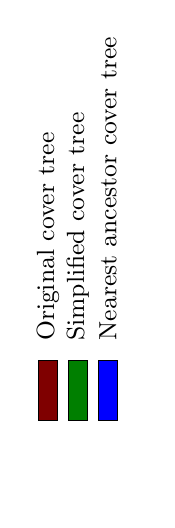
\begin{tikzpicture}
    \node[draw,fill=darkred,minimum width=0.03in,minimum height=0.3in] at (0,0) {};
    \node at (0,0.77in) {\small\rotatebox{90}{Original cover tree}};
    \node[draw,fill=darkgreen,minimum width=0.03in,minimum height=0.3in] at (0.15in,0) {};
    \node at (0.15in,0.82in) {\small\rotatebox{90}{Simplified cover tree}};
    \node[draw,fill=blue,minimum width=0.03in,minimum height=0.3in] at (0.3in,0) {};
    \node at (0.3in,1.01in) {\small\rotatebox{90}{Nearest ancestor cover tree}};
    \node[minimum width=0.05in,minimum height=0.5in] at (0.45in,0) {};
    \node at (0.45in,0.6in) {\small\rotatebox{90}{}};
    \node at (0,-0.5in) {};
\end{tikzpicture}
\end{frame}

%%%%%%%%%%%%%%%%%%%%%%%%%%%%%%%%%%%%%%%%%%%%%%%%%%%%%%%%%%%%%%%%%%%%%%%%%%%%%%%%

\begin{frame}[fragile]{Comparing cover trees on \emph{construction and query} time}
\centering
\graphicspath{{slides/covertree/paperimg/}}
% GNUPLOT: LaTeX picture with Postscript
\begingroup
  \makeatletter
  \providecommand\color[2][]{%
    \GenericError{(gnuplot) \space\space\space\@spaces}{%
      Package color not loaded in conjunction with
      terminal option `colourtext'%
    }{See the gnuplot documentation for explanation.%
    }{Either use 'blacktext' in gnuplot or load the package
      color.sty in LaTeX.}%
    \renewcommand\color[2][]{}%
  }%
  \providecommand\includegraphics[2][]{%
    \GenericError{(gnuplot) \space\space\space\@spaces}{%
      Package graphicx or graphics not loaded%
    }{See the gnuplot documentation for explanation.%
    }{The gnuplot epslatex terminal needs graphicx.sty or graphics.sty.}%
    \renewcommand\includegraphics[2][]{}%
  }%
  \providecommand\rotatebox[2]{#2}%
  \@ifundefined{ifGPcolor}{%
    \newif\ifGPcolor
    \GPcolortrue
  }{}%
  \@ifundefined{ifGPblacktext}{%
    \newif\ifGPblacktext
    \GPblacktextfalse
  }{}%
  % define a \g@addto@macro without @ in the name:
  \let\gplgaddtomacro\g@addto@macro
  % define empty templates for all commands taking text:
  \gdef\gplbacktext{}%
  \gdef\gplfronttext{}%
  \makeatother
  \ifGPblacktext
    % no textcolor at all
    \def\colorrgb#1{}%
    \def\colorgray#1{}%
  \else
    % gray or color?
    \ifGPcolor
      \def\colorrgb#1{\color[rgb]{#1}}%
      \def\colorgray#1{\color[gray]{#1}}%
      \expandafter\def\csname LTw\endcsname{\color{white}}%
      \expandafter\def\csname LTb\endcsname{\color{black}}%
      \expandafter\def\csname LTa\endcsname{\color{black}}%
      \expandafter\def\csname LT0\endcsname{\color[rgb]{1,0,0}}%
      \expandafter\def\csname LT1\endcsname{\color[rgb]{0,1,0}}%
      \expandafter\def\csname LT2\endcsname{\color[rgb]{0,0,1}}%
      \expandafter\def\csname LT3\endcsname{\color[rgb]{1,0,1}}%
      \expandafter\def\csname LT4\endcsname{\color[rgb]{0,1,1}}%
      \expandafter\def\csname LT5\endcsname{\color[rgb]{1,1,0}}%
      \expandafter\def\csname LT6\endcsname{\color[rgb]{0,0,0}}%
      \expandafter\def\csname LT7\endcsname{\color[rgb]{1,0.3,0}}%
      \expandafter\def\csname LT8\endcsname{\color[rgb]{0.5,0.5,0.5}}%
    \else
      % gray
      \def\colorrgb#1{\color{black}}%
      \def\colorgray#1{\color[gray]{#1}}%
      \expandafter\def\csname LTw\endcsname{\color{white}}%
      \expandafter\def\csname LTb\endcsname{\color{black}}%
      \expandafter\def\csname LTa\endcsname{\color{black}}%
      \expandafter\def\csname LT0\endcsname{\color{black}}%
      \expandafter\def\csname LT1\endcsname{\color{black}}%
      \expandafter\def\csname LT2\endcsname{\color{black}}%
      \expandafter\def\csname LT3\endcsname{\color{black}}%
      \expandafter\def\csname LT4\endcsname{\color{black}}%
      \expandafter\def\csname LT5\endcsname{\color{black}}%
      \expandafter\def\csname LT6\endcsname{\color{black}}%
      \expandafter\def\csname LT7\endcsname{\color{black}}%
      \expandafter\def\csname LT8\endcsname{\color{black}}%
    \fi
  \fi
  \setlength{\unitlength}{0.0500bp}%
  \begin{picture}(5040.00,3772.00)%
    \gplgaddtomacro\gplbacktext{%
      \csname LTb\endcsname%
      \put(1122,780){\makebox(0,0)[r]{\strut{} 0}}%
      \put(1122,1235){\makebox(0,0)[r]{\strut{} 0.2}}%
      \put(1122,1689){\makebox(0,0)[r]{\strut{} 0.4}}%
      \put(1122,2144){\makebox(0,0)[r]{\strut{} 0.6}}%
      \put(1122,2598){\makebox(0,0)[r]{\strut{} 0.8}}%
      \put(1122,3052){\makebox(0,0)[r]{\strut{} 1}}%
      \put(1122,3507){\makebox(0,0)[r]{\strut{} 1.2}}%
      \put(1622,648){\rotatebox{-45}{\makebox(0,0)[l]{\strut{}yearpredict}}}%
      \put(1991,648){\rotatebox{-45}{\makebox(0,0)[l]{\strut{}twitter}}}%
      \put(2359,648){\rotatebox{-45}{\makebox(0,0)[l]{\strut{}tinyImages}}}%
      \put(2728,648){\rotatebox{-45}{\makebox(0,0)[l]{\strut{}mnist}}}%
      \put(3096,648){\rotatebox{-45}{\makebox(0,0)[l]{\strut{}corel}}}%
      \put(3465,648){\rotatebox{-45}{\makebox(0,0)[l]{\strut{}covtype}}}%
      \put(3833,648){\rotatebox{-45}{\makebox(0,0)[l]{\strut{}artificial40}}}%
      \put(4202,648){\rotatebox{-45}{\makebox(0,0)[l]{\strut{}faces}}}%
      \put(176,2143){\rotatebox{-270}{\makebox(0,0){\strut{}number of distance comparisons}}}%
      \put(396,2143){\rotatebox{-270}{\makebox(0,0){\strut{}in tree \emph{construction} and \emph{query}}}}%
      \put(616,2143){\rotatebox{-270}{\makebox(0,0){\strut{}(normalized by $n^2$)}}}%
    }%
    \gplgaddtomacro\gplfronttext{%
    }%
    \gplbacktext
    \put(0,0){\includegraphics{numdist}}%
    \gplfronttext
  \end{picture}%
\endgroup

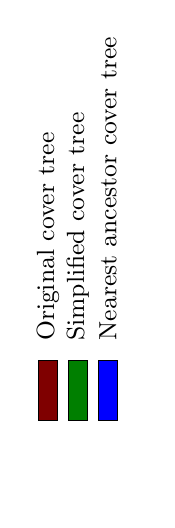
\begin{tikzpicture}
    \node[draw,fill=darkred,minimum width=0.03in,minimum height=0.3in] at (0,0) {};
    \node at (0,0.77in) {\small\rotatebox{90}{Original cover tree}};
    \node[draw,fill=darkgreen,minimum width=0.03in,minimum height=0.3in] at (0.15in,0) {};
    \node at (0.15in,0.82in) {\small\rotatebox{90}{Simplified cover tree}};
    \node[draw,fill=blue,minimum width=0.03in,minimum height=0.3in] at (0.3in,0) {};
    \node at (0.3in,1.01in) {\small\rotatebox{90}{Nearest ancestor cover tree}};
    \node[minimum width=0.05in,minimum height=0.5in] at (0.45in,0) {};
    \node at (0.45in,0.6in) {\small\rotatebox{90}{}};
    \node at (0,-0.5in) {};
\end{tikzpicture}
\end{frame}

%%%%%%%%%%%%%%%%%%%%%%%%%%%%%%%%%%%%%%%%%%%%%%%%%%%%%%%%%%%%%%%%%%%%%%%%%%%%%%%%

\begin{frame}[fragile]{All of the cover trees scale similarly}

This experiment uses the protein data and the random walk graph kernel.
\vspace{0.15in}

{
\centering
\graphicspath{{slides/covertree/paperimg/}}
% GNUPLOT: LaTeX picture with Postscript
\begingroup
  \makeatletter
  \providecommand\color[2][]{%
    \GenericError{(gnuplot) \space\space\space\@spaces}{%
      Package color not loaded in conjunction with
      terminal option `colourtext'%
    }{See the gnuplot documentation for explanation.%
    }{Either use 'blacktext' in gnuplot or load the package
      color.sty in LaTeX.}%
    \renewcommand\color[2][]{}%
  }%
  \providecommand\includegraphics[2][]{%
    \GenericError{(gnuplot) \space\space\space\@spaces}{%
      Package graphicx or graphics not loaded%
    }{See the gnuplot documentation for explanation.%
    }{The gnuplot epslatex terminal needs graphicx.sty or graphics.sty.}%
    \renewcommand\includegraphics[2][]{}%
  }%
  \providecommand\rotatebox[2]{#2}%
  \@ifundefined{ifGPcolor}{%
    \newif\ifGPcolor
    \GPcolortrue
  }{}%
  \@ifundefined{ifGPblacktext}{%
    \newif\ifGPblacktext
    \GPblacktextfalse
  }{}%
  % define a \g@addto@macro without @ in the name:
  \let\gplgaddtomacro\g@addto@macro
  % define empty templates for all commands taking text:
  \gdef\gplbacktext{}%
  \gdef\gplfronttext{}%
  \makeatother
  \ifGPblacktext
    % no textcolor at all
    \def\colorrgb#1{}%
    \def\colorgray#1{}%
  \else
    % gray or color?
    \ifGPcolor
      \def\colorrgb#1{\color[rgb]{#1}}%
      \def\colorgray#1{\color[gray]{#1}}%
      \expandafter\def\csname LTw\endcsname{\color{white}}%
      \expandafter\def\csname LTb\endcsname{\color{black}}%
      \expandafter\def\csname LTa\endcsname{\color{black}}%
      \expandafter\def\csname LT0\endcsname{\color[rgb]{1,0,0}}%
      \expandafter\def\csname LT1\endcsname{\color[rgb]{0,1,0}}%
      \expandafter\def\csname LT2\endcsname{\color[rgb]{0,0,1}}%
      \expandafter\def\csname LT3\endcsname{\color[rgb]{1,0,1}}%
      \expandafter\def\csname LT4\endcsname{\color[rgb]{0,1,1}}%
      \expandafter\def\csname LT5\endcsname{\color[rgb]{1,1,0}}%
      \expandafter\def\csname LT6\endcsname{\color[rgb]{0,0,0}}%
      \expandafter\def\csname LT7\endcsname{\color[rgb]{1,0.3,0}}%
      \expandafter\def\csname LT8\endcsname{\color[rgb]{0.5,0.5,0.5}}%
    \else
      % gray
      \def\colorrgb#1{\color{black}}%
      \def\colorgray#1{\color[gray]{#1}}%
      \expandafter\def\csname LTw\endcsname{\color{white}}%
      \expandafter\def\csname LTb\endcsname{\color{black}}%
      \expandafter\def\csname LTa\endcsname{\color{black}}%
      \expandafter\def\csname LT0\endcsname{\color{black}}%
      \expandafter\def\csname LT1\endcsname{\color{black}}%
      \expandafter\def\csname LT2\endcsname{\color{black}}%
      \expandafter\def\csname LT3\endcsname{\color{black}}%
      \expandafter\def\csname LT4\endcsname{\color{black}}%
      \expandafter\def\csname LT5\endcsname{\color{black}}%
      \expandafter\def\csname LT6\endcsname{\color{black}}%
      \expandafter\def\csname LT7\endcsname{\color{black}}%
      \expandafter\def\csname LT8\endcsname{\color{black}}%
    \fi
  \fi
  \setlength{\unitlength}{0.0500bp}%
  \begin{picture}(5040.00,3772.00)%
    \gplgaddtomacro\gplbacktext{%
      \csname LTb\endcsname%
      \put(1298,704){\makebox(0,0)[r]{\strut{} 0}}%
      \put(1298,1054){\makebox(0,0)[r]{\strut{} 200}}%
      \put(1298,1405){\makebox(0,0)[r]{\strut{} 400}}%
      \put(1298,1755){\makebox(0,0)[r]{\strut{} 600}}%
      \put(1298,2106){\makebox(0,0)[r]{\strut{} 800}}%
      \put(1298,2456){\makebox(0,0)[r]{\strut{} 1000}}%
      \put(1298,2806){\makebox(0,0)[r]{\strut{} 1200}}%
      \put(1298,3157){\makebox(0,0)[r]{\strut{} 1400}}%
      \put(1298,3507){\makebox(0,0)[r]{\strut{} 1600}}%
      \put(1430,484){\makebox(0,0){\strut{} 0}}%
      \put(2073,484){\makebox(0,0){\strut{} 50}}%
      \put(2715,484){\makebox(0,0){\strut{} 100}}%
      \put(3358,484){\makebox(0,0){\strut{} 150}}%
      \put(4000,484){\makebox(0,0){\strut{} 200}}%
      \put(4643,484){\makebox(0,0){\strut{} 250}}%
      \put(176,2105){\rotatebox{-270}{\makebox(0,0){\strut{}total distance comparisons (millions)}}}%
      \put(396,2105){\rotatebox{-270}{\makebox(0,0){\strut{}on \emph{construction} and \emph{query}}}}%
      \put(3036,154){\makebox(0,0){\strut{}number of data points (thousands)}}%
    }%
    \gplgaddtomacro\gplfronttext{%
    }%
    \gplbacktext
    \put(0,0){\includegraphics{protein-simple}}%
    \gplfronttext
  \end{picture}%
\endgroup

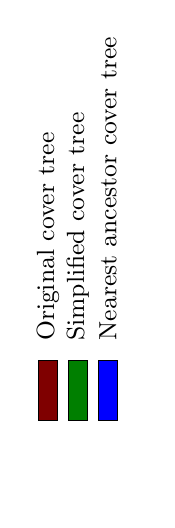
\begin{tikzpicture}
    \node[draw,fill=darkred,minimum width=0.03in,minimum height=0.3in] at (0,0) {};
    \node at (0,0.77in) {\small\rotatebox{90}{Original cover tree}};
    \node[draw,fill=darkgreen,minimum width=0.03in,minimum height=0.3in] at (0.15in,0) {};
    \node at (0.15in,0.82in) {\small\rotatebox{90}{Simplified cover tree}};
    \node[draw,fill=blue,minimum width=0.03in,minimum height=0.3in] at (0.3in,0) {};
    \node at (0.3in,1.01in) {\small\rotatebox{90}{Nearest ancestor cover tree}};
    \node[minimum width=0.05in,minimum height=0.5in] at (0.45in,0) {};
    %\node at (0.6in,0.7in) {\small\rotatebox{90}{ dotted lines: construction only}};
    %\node at (0.75in,0.81in) {\small\rotatebox{90}{ solid lines: construction and query}};
    \node at (0,-0.5in) {};
\end{tikzpicture}
}

\end{frame}

\begin{frame}[fragile]{Cache oblivious cover tree}

%RAM model is a lie
%
%\vspace{0.1in}
Need to consider cache accesses for fast, modern data structures

%\vspace{0.1in}
%In a \emph{cache oblivious} data structure, the programmer doesn't need to know any details about the underlying hardware
%
\begin{center}
\includegraphics[width=10cm]{slides/covertree/cpu_cache_structure}
\end{center}

{\tiny image from: \url{http://1024cores.net} }
\end{frame}

%%%%%%%%%%%%%%%%%%%%%%%%%%%%%%%%%%%%%%%%%%%%%%%%%%%%%%%%%%%%%%%%%%%%%%%%%%%%%%%%

\begin{frame}[fragile]{Cache oblivious cover tree}

%The trick: use the van Emde Boas tree layout
Arrange nodes in memory according to a preorder traversal of the tree

(van Emde Boas \emph{et al.}, 1966; Demaine, 2002)
\vspace{0.1in}

\begin{center}
\includegraphics[width=6cm]{slides/covertree/preorder.png}
\end{center}

{\tiny image from: Wikipedia}
%(nodes arranged in memory according to a pre-order depth first traversal)
%
%\vspace{-0.1in}
%%{
%%\centering
%\begin{center}
%\includegraphics[width=8cm]{covertree/cache_oblivious_divide}
%\end{center}
%%}
%
%\vspace{-0.1in}
%Optimal cache performance without any knowledge of the architecture
%\vspace{0.15in}

%source: 1024cores.net

\end{frame}

%%%%%%%%%%%%%%%%%%%%%%%%%%%%%%%%%%%%%%%%%%%%%%%%%%%%%%%%%%%%%%%%%%%%%%%%%%%%%%%%

\begin{frame}[fragile]{The cache efficiency of three cover tree implementations}

\centering
\graphicspath{{slides/covertree/paperimg/}}
% GNUPLOT: LaTeX picture with Postscript
\begingroup
  \makeatletter
  \providecommand\color[2][]{%
    \GenericError{(gnuplot) \space\space\space\@spaces}{%
      Package color not loaded in conjunction with
      terminal option `colourtext'%
    }{See the gnuplot documentation for explanation.%
    }{Either use 'blacktext' in gnuplot or load the package
      color.sty in LaTeX.}%
    \renewcommand\color[2][]{}%
  }%
  \providecommand\includegraphics[2][]{%
    \GenericError{(gnuplot) \space\space\space\@spaces}{%
      Package graphicx or graphics not loaded%
    }{See the gnuplot documentation for explanation.%
    }{The gnuplot epslatex terminal needs graphicx.sty or graphics.sty.}%
    \renewcommand\includegraphics[2][]{}%
  }%
  \providecommand\rotatebox[2]{#2}%
  \@ifundefined{ifGPcolor}{%
    \newif\ifGPcolor
    \GPcolortrue
  }{}%
  \@ifundefined{ifGPblacktext}{%
    \newif\ifGPblacktext
    \GPblacktextfalse
  }{}%
  % define a \g@addto@macro without @ in the name:
  \let\gplgaddtomacro\g@addto@macro
  % define empty templates for all commands taking text:
  \gdef\gplbacktext{}%
  \gdef\gplfronttext{}%
  \makeatother
  \ifGPblacktext
    % no textcolor at all
    \def\colorrgb#1{}%
    \def\colorgray#1{}%
  \else
    % gray or color?
    \ifGPcolor
      \def\colorrgb#1{\color[rgb]{#1}}%
      \def\colorgray#1{\color[gray]{#1}}%
      \expandafter\def\csname LTw\endcsname{\color{white}}%
      \expandafter\def\csname LTb\endcsname{\color{black}}%
      \expandafter\def\csname LTa\endcsname{\color{black}}%
      \expandafter\def\csname LT0\endcsname{\color[rgb]{1,0,0}}%
      \expandafter\def\csname LT1\endcsname{\color[rgb]{0,1,0}}%
      \expandafter\def\csname LT2\endcsname{\color[rgb]{0,0,1}}%
      \expandafter\def\csname LT3\endcsname{\color[rgb]{1,0,1}}%
      \expandafter\def\csname LT4\endcsname{\color[rgb]{0,1,1}}%
      \expandafter\def\csname LT5\endcsname{\color[rgb]{1,1,0}}%
      \expandafter\def\csname LT6\endcsname{\color[rgb]{0,0,0}}%
      \expandafter\def\csname LT7\endcsname{\color[rgb]{1,0.3,0}}%
      \expandafter\def\csname LT8\endcsname{\color[rgb]{0.5,0.5,0.5}}%
    \else
      % gray
      \def\colorrgb#1{\color{black}}%
      \def\colorgray#1{\color[gray]{#1}}%
      \expandafter\def\csname LTw\endcsname{\color{white}}%
      \expandafter\def\csname LTb\endcsname{\color{black}}%
      \expandafter\def\csname LTa\endcsname{\color{black}}%
      \expandafter\def\csname LT0\endcsname{\color{black}}%
      \expandafter\def\csname LT1\endcsname{\color{black}}%
      \expandafter\def\csname LT2\endcsname{\color{black}}%
      \expandafter\def\csname LT3\endcsname{\color{black}}%
      \expandafter\def\csname LT4\endcsname{\color{black}}%
      \expandafter\def\csname LT5\endcsname{\color{black}}%
      \expandafter\def\csname LT6\endcsname{\color{black}}%
      \expandafter\def\csname LT7\endcsname{\color{black}}%
      \expandafter\def\csname LT8\endcsname{\color{black}}%
    \fi
  \fi
  \setlength{\unitlength}{0.0500bp}%
  \begin{picture}(5040.00,3772.00)%
    \gplgaddtomacro\gplbacktext{%
      \csname LTb\endcsname%
      \put(1166,780){\makebox(0,0)[r]{\strut{} 0}}%
      \put(1166,1325){\makebox(0,0)[r]{\strut{} 0.2}}%
      \put(1166,1871){\makebox(0,0)[r]{\strut{} 0.4}}%
      \put(1166,2416){\makebox(0,0)[r]{\strut{} 0.6}}%
      \put(1166,2962){\makebox(0,0)[r]{\strut{} 0.8}}%
      \put(1166,3507){\makebox(0,0)[r]{\strut{} 1}}%
      \put(1661,648){\rotatebox{-45}{\makebox(0,0)[l]{\strut{}yearpredict}}}%
      \put(2023,648){\rotatebox{-45}{\makebox(0,0)[l]{\strut{}twitter}}}%
      \put(2386,648){\rotatebox{-45}{\makebox(0,0)[l]{\strut{}tinyImages}}}%
      \put(2748,648){\rotatebox{-45}{\makebox(0,0)[l]{\strut{}mnist}}}%
      \put(3111,648){\rotatebox{-45}{\makebox(0,0)[l]{\strut{}corel}}}%
      \put(3473,648){\rotatebox{-45}{\makebox(0,0)[l]{\strut{}covtype}}}%
      \put(3836,648){\rotatebox{-45}{\makebox(0,0)[l]{\strut{}artificial40}}}%
      \put(4198,648){\rotatebox{-45}{\makebox(0,0)[l]{\strut{}faces}}}%
      \put(176,2143){\rotatebox{-270}{\makebox(0,0){\strut{}cache miss rate}}}%
      \put(396,2143){\rotatebox{-270}{\makebox(0,0){\strut{}(cache misses / cache accesses)}}}%
    }%
    \gplgaddtomacro\gplfronttext{%
    }%
    \gplbacktext
    \put(0,0){\includegraphics{cache-hlearn}}%
    \gplfronttext
  \end{picture}%
\endgroup

\definecolor{colorOrig}{RGB}{102,51,0}
\definecolor{colorMlpack}{RGB}{204,153,0}
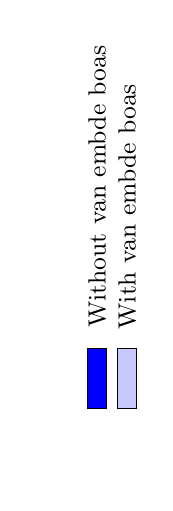
\begin{tikzpicture}
    %\node[draw,fill=colorOrig,minimum width=0.05in,minimum height=0.3in] at (0,0) {};
    %\node at (0,0.79in) {\small\rotatebox{90}{Reference cover tree}};
    %\node[draw,fill=colorMlpack,minimum width=0.05in,minimum height=0.3in] at (0.15in,0) {};
    %\node at (0.15in,0.79in) {\small\rotatebox{90}{MLPack's cover tree}};
    %\node[draw,fill=blue,minimum width=0.05in,minimum height=0.3in] at (0.3in,0) {};
    %\node at (0.3in,0.98in) {\small\rotatebox{90}{Our cover tree (unpacked)}};
    %\node[draw,fill=lightblue,minimum width=0.05in,minimum height=0.3in] at (0.45in,0) {};
    %\node at (0.45in,0.91in) {\small\rotatebox{90}{Our cover tree (packed)}};
    \node[draw,fill=blue,minimum width=0.05in,minimum height=0.3in] at (0.3in,0) {};
    \node at (0.3in,0.98in) {\small\rotatebox{90}{Without van embde boas }};
    \node[draw,fill=lightblue,minimum width=0.05in,minimum height=0.3in] at (0.45in,0) {};
    \node at (0.45in,0.88in) {\small\rotatebox{90}{With van embde boas }};
    \node at (0,-0.475in) {};
\end{tikzpicture}

\vspace{0.15in}
Measured using Linux's \lstinline{perf stat} utility on an Amazon AWS instance
\end{frame}

%%%%%%%%%%%%%%%%%%%%%%%%%%%%%%%%%%%%%%%%%%%%%%%%%%%%%%%%%%%%%%%%%%%%%%%%%%%%%%%%
%
%\begin{frame}[fragile]{The cache efficiency of three cover tree implementations}
%
%\centering
%\graphicspath{{slides/covertree/paperimg/}}
%% GNUPLOT: LaTeX picture with Postscript
\begingroup
  \makeatletter
  \providecommand\color[2][]{%
    \GenericError{(gnuplot) \space\space\space\@spaces}{%
      Package color not loaded in conjunction with
      terminal option `colourtext'%
    }{See the gnuplot documentation for explanation.%
    }{Either use 'blacktext' in gnuplot or load the package
      color.sty in LaTeX.}%
    \renewcommand\color[2][]{}%
  }%
  \providecommand\includegraphics[2][]{%
    \GenericError{(gnuplot) \space\space\space\@spaces}{%
      Package graphicx or graphics not loaded%
    }{See the gnuplot documentation for explanation.%
    }{The gnuplot epslatex terminal needs graphicx.sty or graphics.sty.}%
    \renewcommand\includegraphics[2][]{}%
  }%
  \providecommand\rotatebox[2]{#2}%
  \@ifundefined{ifGPcolor}{%
    \newif\ifGPcolor
    \GPcolortrue
  }{}%
  \@ifundefined{ifGPblacktext}{%
    \newif\ifGPblacktext
    \GPblacktextfalse
  }{}%
  % define a \g@addto@macro without @ in the name:
  \let\gplgaddtomacro\g@addto@macro
  % define empty templates for all commands taking text:
  \gdef\gplbacktext{}%
  \gdef\gplfronttext{}%
  \makeatother
  \ifGPblacktext
    % no textcolor at all
    \def\colorrgb#1{}%
    \def\colorgray#1{}%
  \else
    % gray or color?
    \ifGPcolor
      \def\colorrgb#1{\color[rgb]{#1}}%
      \def\colorgray#1{\color[gray]{#1}}%
      \expandafter\def\csname LTw\endcsname{\color{white}}%
      \expandafter\def\csname LTb\endcsname{\color{black}}%
      \expandafter\def\csname LTa\endcsname{\color{black}}%
      \expandafter\def\csname LT0\endcsname{\color[rgb]{1,0,0}}%
      \expandafter\def\csname LT1\endcsname{\color[rgb]{0,1,0}}%
      \expandafter\def\csname LT2\endcsname{\color[rgb]{0,0,1}}%
      \expandafter\def\csname LT3\endcsname{\color[rgb]{1,0,1}}%
      \expandafter\def\csname LT4\endcsname{\color[rgb]{0,1,1}}%
      \expandafter\def\csname LT5\endcsname{\color[rgb]{1,1,0}}%
      \expandafter\def\csname LT6\endcsname{\color[rgb]{0,0,0}}%
      \expandafter\def\csname LT7\endcsname{\color[rgb]{1,0.3,0}}%
      \expandafter\def\csname LT8\endcsname{\color[rgb]{0.5,0.5,0.5}}%
    \else
      % gray
      \def\colorrgb#1{\color{black}}%
      \def\colorgray#1{\color[gray]{#1}}%
      \expandafter\def\csname LTw\endcsname{\color{white}}%
      \expandafter\def\csname LTb\endcsname{\color{black}}%
      \expandafter\def\csname LTa\endcsname{\color{black}}%
      \expandafter\def\csname LT0\endcsname{\color{black}}%
      \expandafter\def\csname LT1\endcsname{\color{black}}%
      \expandafter\def\csname LT2\endcsname{\color{black}}%
      \expandafter\def\csname LT3\endcsname{\color{black}}%
      \expandafter\def\csname LT4\endcsname{\color{black}}%
      \expandafter\def\csname LT5\endcsname{\color{black}}%
      \expandafter\def\csname LT6\endcsname{\color{black}}%
      \expandafter\def\csname LT7\endcsname{\color{black}}%
      \expandafter\def\csname LT8\endcsname{\color{black}}%
    \fi
  \fi
  \setlength{\unitlength}{0.0500bp}%
  \begin{picture}(5040.00,3772.00)%
    \gplgaddtomacro\gplbacktext{%
      \csname LTb\endcsname%
      \put(1166,780){\makebox(0,0)[r]{\strut{} 0}}%
      \put(1166,1325){\makebox(0,0)[r]{\strut{} 0.2}}%
      \put(1166,1871){\makebox(0,0)[r]{\strut{} 0.4}}%
      \put(1166,2416){\makebox(0,0)[r]{\strut{} 0.6}}%
      \put(1166,2962){\makebox(0,0)[r]{\strut{} 0.8}}%
      \put(1166,3507){\makebox(0,0)[r]{\strut{} 1}}%
      \put(1661,648){\rotatebox{-45}{\makebox(0,0)[l]{\strut{}yearpredict}}}%
      \put(2023,648){\rotatebox{-45}{\makebox(0,0)[l]{\strut{}twitter}}}%
      \put(2386,648){\rotatebox{-45}{\makebox(0,0)[l]{\strut{}tinyImages}}}%
      \put(2748,648){\rotatebox{-45}{\makebox(0,0)[l]{\strut{}mnist}}}%
      \put(3111,648){\rotatebox{-45}{\makebox(0,0)[l]{\strut{}corel}}}%
      \put(3473,648){\rotatebox{-45}{\makebox(0,0)[l]{\strut{}covtype}}}%
      \put(3836,648){\rotatebox{-45}{\makebox(0,0)[l]{\strut{}artificial40}}}%
      \put(4198,648){\rotatebox{-45}{\makebox(0,0)[l]{\strut{}faces}}}%
      \put(176,2143){\rotatebox{-270}{\makebox(0,0){\strut{}stalled CPU cycle rate}}}%
      \put(396,2143){\rotatebox{-270}{\makebox(0,0){\strut{}(stalled cycles / total cycles)}}}%
    }%
    \gplgaddtomacro\gplfronttext{%
    }%
    \gplbacktext
    \put(0,0){\includegraphics{stalled-front}}%
    \gplfronttext
  \end{picture}%
\endgroup

%\definecolor{colorOrig}{RGB}{102,51,0}
%\definecolor{colorMlpack}{RGB}{204,153,0}
%\begin{tikzpicture}
    %\node[draw,fill=colorOrig,minimum width=0.05in,minimum height=0.3in] at (0,0) {};
    %\node at (0,0.79in) {\small\rotatebox{90}{Reference cover tree}};
    %\node[draw,fill=colorMlpack,minimum width=0.05in,minimum height=0.3in] at (0.15in,0) {};
    %\node at (0.15in,0.79in) {\small\rotatebox{90}{MLPack's cover tree}};
    %\node[draw,fill=blue,minimum width=0.05in,minimum height=0.3in] at (0.3in,0) {};
    %\node at (0.3in,0.98in) {\small\rotatebox{90}{Our cover tree (unpacked)}};
    %\node[draw,fill=lightblue,minimum width=0.05in,minimum height=0.3in] at (0.45in,0) {};
    %\node at (0.45in,0.91in) {\small\rotatebox{90}{Our cover tree (packed)}};
    %\node at (0,-0.475in) {};
%\end{tikzpicture}
%
%\vspace{0.15in}
%Measured using Linux's \lstinline{perf stat} utility on an Amazon AWS instance
%\end{frame}

\begin{frame}[fragile]{Merging cover trees}

Merging cover trees gives us a parallel tree construction algorithm

\vspace{0.15in}

Sometimes, merging cover trees is \textbf{easy}:

\begin{center}
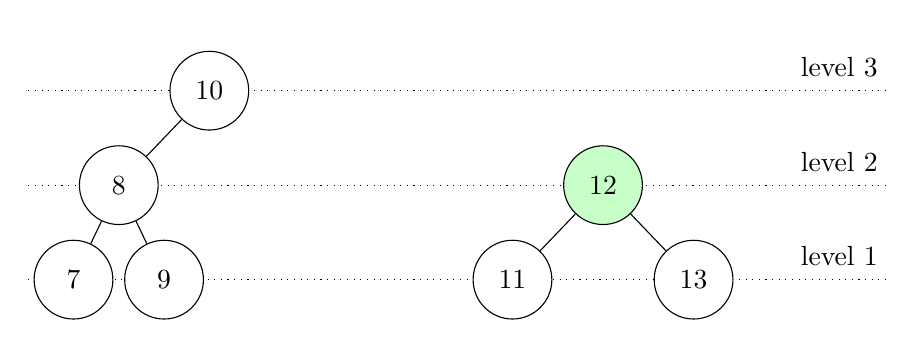
\begin{tikzpicture}
    [ draw
    , every node/.style={minimum size=10mm,fill=white}
    , level/.style={sibling distance = 23mm/#1, level distance=12mm}
    %,    level distance = 1.5cm}
    , sibling distance=8mm
    ]
\draw (-2.3,0) -- (8.6,0)[dotted];
\draw (-2.3,-12mm) -- (8.6,-12mm)[dotted];
\draw (-2.3,-24mm) -- (8.6,-24mm)[dotted];
\node[shape=circle,draw] at (0,0) {10}
    child { node[circle,draw] {8}
        child { node[circle,draw] {7}  }
        child { node[circle,draw] {9} }
        }
    child [color=white] {}
    %child { node[circle,draw] {12}
        %child { node[circle,draw] {9}  }
        %child { node[circle,draw] {13} }
        %}
    ;
\node[shape=circle,draw,fill=lightgreen] at (5,-12mm) {12}
    %child { node[circle,draw] {8}
        %child { node[circle,draw] {7}  }
        %child { node[circle,draw,fill=lightgreen,line width=1pt] {9} }
        %}
    %child { node[circle,draw] {12}
        child { node[circle,draw] {11}  }
        child { node[circle,draw] {13} }
        %}
    ;
\node[fill=none] at (8,3mm) {level 3};
\node[fill=none] at (8,-9mm) {level 2};
\node[fill=none] at (8,-21mm) {level 1};
\end{tikzpicture}
\end{center}

\vspace{0.1in}
No runtime bound on the merge operation, but it is fast in practice

%\vspace{0.1in}
%But, if the runtime is $o(n)$, then we get an algorithm for tree construction that takes time $O(n)$
\end{frame}

%%%%%%%%%%%%%%%%%%%%%%%%%%%%%%%%%%%%%%%%%%%%%%%%%%%%%%%%%%%%%%%%%%%%%%%%%%%%%%%%

\begin{frame}[fragile]{Merging cover trees}

Merging cover trees gives us a parallel tree construction algorithm

\vspace{0.15in}

Sometimes, merging cover trees is \textbf{hard}:

\begin{center}
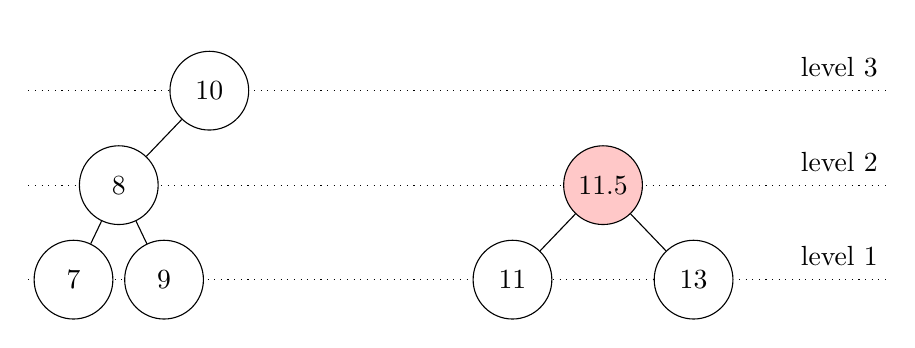
\begin{tikzpicture}
    [ draw
    , every node/.style={minimum size=10mm,fill=white}
    , level/.style={sibling distance = 23mm/#1, level distance=12mm}
    %,    level distance = 1.5cm}
    , sibling distance=8mm
    ]
\draw (-2.3,0) -- (8.6,0)[dotted];
\draw (-2.3,-12mm) -- (8.6,-12mm)[dotted];
\draw (-2.3,-24mm) -- (8.6,-24mm)[dotted];
\node[shape=circle,draw] at (0,0) {10}
    child { node[circle,draw] {8}
        child { node[circle,draw] {7}  }
        child { node[circle,draw] {9} }
        }
    child [color=white] {}
    %child { node[circle,draw] {12}
        %child { node[circle,draw] {9}  }
        %child { node[circle,draw] {13} }
        %}
    ;
\node[shape=circle,draw,fill=lightred] at (5,-12mm) {11.5}
    %child { node[circle,draw] {8}
        %child { node[circle,draw] {7}  }
        %child { node[circle,draw,fill=lightgreen,line width=1pt] {9} }
        %}
    %child { node[circle,draw] {12}
        child { node[circle,draw] {11}  }
        child { node[circle,draw] {13} }
        %}
    ;
\node[fill=none] at (8,3mm) {level 3};
\node[fill=none] at (8,-9mm) {level 2};
\node[fill=none] at (8,-21mm) {level 1};
\end{tikzpicture}
\end{center}

\vspace{0.1in}
No runtime bound on the merge operation, but it is fast in practice

%\vspace{0.1in}
%But, if the runtime is $o(n)$, then we get an algorithm for tree construction that takes time $O(n)$
\end{frame}

%%%%%%%%%%%%%%%%%%%%%%%%%%%%%%%%%%%%%%%%%%%%%%%%%%%%%%%%%%%%%%%%%%%%%%%%%%%%%%%%

\begin{frame}[fragile]{The effect of parallel tree \emph{construction} on small datasets}
\begin{center}
\graphicspath{{slides/covertree/paperimg/}}
% GNUPLOT: LaTeX picture with Postscript
\begingroup
  \makeatletter
  \providecommand\color[2][]{%
    \GenericError{(gnuplot) \space\space\space\@spaces}{%
      Package color not loaded in conjunction with
      terminal option `colourtext'%
    }{See the gnuplot documentation for explanation.%
    }{Either use 'blacktext' in gnuplot or load the package
      color.sty in LaTeX.}%
    \renewcommand\color[2][]{}%
  }%
  \providecommand\includegraphics[2][]{%
    \GenericError{(gnuplot) \space\space\space\@spaces}{%
      Package graphicx or graphics not loaded%
    }{See the gnuplot documentation for explanation.%
    }{The gnuplot epslatex terminal needs graphicx.sty or graphics.sty.}%
    \renewcommand\includegraphics[2][]{}%
  }%
  \providecommand\rotatebox[2]{#2}%
  \@ifundefined{ifGPcolor}{%
    \newif\ifGPcolor
    \GPcolortrue
  }{}%
  \@ifundefined{ifGPblacktext}{%
    \newif\ifGPblacktext
    \GPblacktextfalse
  }{}%
  % define a \g@addto@macro without @ in the name:
  \let\gplgaddtomacro\g@addto@macro
  % define empty templates for all commands taking text:
  \gdef\gplbacktext{}%
  \gdef\gplfronttext{}%
  \makeatother
  \ifGPblacktext
    % no textcolor at all
    \def\colorrgb#1{}%
    \def\colorgray#1{}%
  \else
    % gray or color?
    \ifGPcolor
      \def\colorrgb#1{\color[rgb]{#1}}%
      \def\colorgray#1{\color[gray]{#1}}%
      \expandafter\def\csname LTw\endcsname{\color{white}}%
      \expandafter\def\csname LTb\endcsname{\color{black}}%
      \expandafter\def\csname LTa\endcsname{\color{black}}%
      \expandafter\def\csname LT0\endcsname{\color[rgb]{1,0,0}}%
      \expandafter\def\csname LT1\endcsname{\color[rgb]{0,1,0}}%
      \expandafter\def\csname LT2\endcsname{\color[rgb]{0,0,1}}%
      \expandafter\def\csname LT3\endcsname{\color[rgb]{1,0,1}}%
      \expandafter\def\csname LT4\endcsname{\color[rgb]{0,1,1}}%
      \expandafter\def\csname LT5\endcsname{\color[rgb]{1,1,0}}%
      \expandafter\def\csname LT6\endcsname{\color[rgb]{0,0,0}}%
      \expandafter\def\csname LT7\endcsname{\color[rgb]{1,0.3,0}}%
      \expandafter\def\csname LT8\endcsname{\color[rgb]{0.5,0.5,0.5}}%
    \else
      % gray
      \def\colorrgb#1{\color{black}}%
      \def\colorgray#1{\color[gray]{#1}}%
      \expandafter\def\csname LTw\endcsname{\color{white}}%
      \expandafter\def\csname LTb\endcsname{\color{black}}%
      \expandafter\def\csname LTa\endcsname{\color{black}}%
      \expandafter\def\csname LT0\endcsname{\color{black}}%
      \expandafter\def\csname LT1\endcsname{\color{black}}%
      \expandafter\def\csname LT2\endcsname{\color{black}}%
      \expandafter\def\csname LT3\endcsname{\color{black}}%
      \expandafter\def\csname LT4\endcsname{\color{black}}%
      \expandafter\def\csname LT5\endcsname{\color{black}}%
      \expandafter\def\csname LT6\endcsname{\color{black}}%
      \expandafter\def\csname LT7\endcsname{\color{black}}%
      \expandafter\def\csname LT8\endcsname{\color{black}}%
    \fi
  \fi
  \setlength{\unitlength}{0.0500bp}%
  \begin{picture}(5040.00,3772.00)%
    \gplgaddtomacro\gplbacktext{%
      \csname LTb\endcsname%
      \put(814,1129){\makebox(0,0)[r]{\strut{}$2^{-4}$}}%
      \csname LTb\endcsname%
      \put(814,1526){\makebox(0,0)[r]{\strut{}$2^{-3}$}}%
      \csname LTb\endcsname%
      \put(814,1922){\makebox(0,0)[r]{\strut{}$2^{-2}$}}%
      \csname LTb\endcsname%
      \put(814,2318){\makebox(0,0)[r]{\strut{}$2^{-1}$}}%
      \csname LTb\endcsname%
      \put(814,2714){\makebox(0,0)[r]{\strut{}$2^{+0}$}}%
      \csname LTb\endcsname%
      \put(814,3111){\makebox(0,0)[r]{\strut{}$2^{+1}$}}%
      \put(1539,601){\rotatebox{-45}{\makebox(0,0)[l]{\strut{}yearpredict}}}%
      \put(1539,381){\rotatebox{-45}{\makebox(0,0)[l]{\strut{}(77sec)}}}%
      \put(2242,601){\rotatebox{-45}{\makebox(0,0)[l]{\strut{}twitter}}}%
      \put(2242,381){\rotatebox{-45}{\makebox(0,0)[l]{\strut{}(107sec)}}}%
      \put(2945,601){\rotatebox{-45}{\makebox(0,0)[l]{\strut{}tinyImages}}}%
      \put(2945,381){\rotatebox{-45}{\makebox(0,0)[l]{\strut{}(65sec)}}}%
      \put(3648,601){\rotatebox{-45}{\makebox(0,0)[l]{\strut{}mnist}}}%
      \put(3648,381){\rotatebox{-45}{\makebox(0,0)[l]{\strut{}(12sec)}}}%
      \put(176,2120){\rotatebox{-270}{\makebox(0,0){\strut{}normalized tree \emph{construction} time}}}%
      \put(1464,2814){\makebox(0,0)[l]{\strut{}\tiny 1}}%
      \put(1570,2619){\makebox(0,0)[l]{\strut{}\tiny 2}}%
      \put(1667,2175){\makebox(0,0)[l]{\strut{}\tiny 4}}%
      \put(1763,1967){\makebox(0,0)[l]{\strut{}\tiny 8}}%
      \put(1860,1856){\makebox(0,0)[l]{\strut{}\tiny 16}}%
      \put(1473,3230){\makebox(0,0)[l]{\strut{}number of processors}}%
    }%
    \gplgaddtomacro\gplfronttext{%
    }%
    \gplbacktext
    \put(0,0){\includegraphics{parallel-ancestor-build}}%
    \gplfronttext
  \end{picture}%
\endgroup

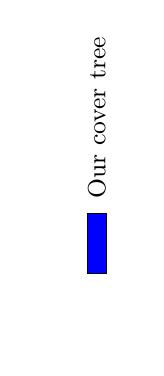
\begin{tikzpicture}
    \node[draw,fill=blue,minimum width=0.05in,minimum height=0.3in] at (0.3in,0) {};
    \node at (0.3in,0.63in) {\small\rotatebox{90}{Our cover tree}};
    \node[minimum width=0.05in,minimum height=0.3in] at (0.45in,0) {};
    \node at (0.45in,0.61in) {\small\rotatebox{90}{}};
    \node at (0,-0.475in) {};
\end{tikzpicture}
\end{center}

\vspace{0.1in}
Experiments run on an Amazon AWS instance with 16 true cores
\end{frame}

%%%%%%%%%%%%%%%%%%%%%%%%%%%%%%%%%%%%%%%%%%%%%%%%%%%%%%%%%%%%%%%%%%%%%%%%%%%%%%%%

\begin{frame}[fragile]{Parallel tree construction really matters on larger data sets}


%on small datasets with cheap metrics, parallel construction is less useful

\vspace{0.1in}
On large datasets with an expensive metric, parallelism is more useful

\vspace{0.15in}
Yahoo! Flickr dataset with 1.5 million images and earth mover distance

%\vspace{0.2in}
\vspace{0.15in}
\begin{center}
\Large
\begin{tabular}{ccccc}
\hline
num cores
 & \multicolumn{2}{c}{simplified tree} & \multicolumn{2}{c}{nearest ancestor tree} \\
%& \multicolumn{2}{c}{construction} & \multicolumn{2}{c}{construction} \\ %\cline{2-5}
& time & speedup & time & speedup \\
\hline
\hline
1  & 70.7 min & 1.0 & 210.9 min& 1.0\\
2  & 36.6 min & 1.9 & 94.2 min & 2.2\\
4  & 18.5 min & 3.8 & 48.5 min & 4.3\\
8  & 10.2 min & 6.9 & 25.3 min & 8.3\\
16 & 6.7 min & 10.5 & 12.0 min & 17.6\\
\hline
\end{tabular}
\end{center}

\end{frame}

%%%%%%%%%%%%%%%%%%%%%%%%%%%%%%%%%%%%%%%%%%%%%%%%%%%%%%%%%%%%%%%%%%%%%%%%%%%%%%%%

\begin{frame}[fragile]{The effect of parallel tree \emph{construction and query}}
\begin{center}
\graphicspath{{slides/covertree/paperimg/}}
% GNUPLOT: LaTeX picture with Postscript
\begingroup
  \makeatletter
  \providecommand\color[2][]{%
    \GenericError{(gnuplot) \space\space\space\@spaces}{%
      Package color not loaded in conjunction with
      terminal option `colourtext'%
    }{See the gnuplot documentation for explanation.%
    }{Either use 'blacktext' in gnuplot or load the package
      color.sty in LaTeX.}%
    \renewcommand\color[2][]{}%
  }%
  \providecommand\includegraphics[2][]{%
    \GenericError{(gnuplot) \space\space\space\@spaces}{%
      Package graphicx or graphics not loaded%
    }{See the gnuplot documentation for explanation.%
    }{The gnuplot epslatex terminal needs graphicx.sty or graphics.sty.}%
    \renewcommand\includegraphics[2][]{}%
  }%
  \providecommand\rotatebox[2]{#2}%
  \@ifundefined{ifGPcolor}{%
    \newif\ifGPcolor
    \GPcolortrue
  }{}%
  \@ifundefined{ifGPblacktext}{%
    \newif\ifGPblacktext
    \GPblacktextfalse
  }{}%
  % define a \g@addto@macro without @ in the name:
  \let\gplgaddtomacro\g@addto@macro
  % define empty templates for all commands taking text:
  \gdef\gplbacktext{}%
  \gdef\gplfronttext{}%
  \makeatother
  \ifGPblacktext
    % no textcolor at all
    \def\colorrgb#1{}%
    \def\colorgray#1{}%
  \else
    % gray or color?
    \ifGPcolor
      \def\colorrgb#1{\color[rgb]{#1}}%
      \def\colorgray#1{\color[gray]{#1}}%
      \expandafter\def\csname LTw\endcsname{\color{white}}%
      \expandafter\def\csname LTb\endcsname{\color{black}}%
      \expandafter\def\csname LTa\endcsname{\color{black}}%
      \expandafter\def\csname LT0\endcsname{\color[rgb]{1,0,0}}%
      \expandafter\def\csname LT1\endcsname{\color[rgb]{0,1,0}}%
      \expandafter\def\csname LT2\endcsname{\color[rgb]{0,0,1}}%
      \expandafter\def\csname LT3\endcsname{\color[rgb]{1,0,1}}%
      \expandafter\def\csname LT4\endcsname{\color[rgb]{0,1,1}}%
      \expandafter\def\csname LT5\endcsname{\color[rgb]{1,1,0}}%
      \expandafter\def\csname LT6\endcsname{\color[rgb]{0,0,0}}%
      \expandafter\def\csname LT7\endcsname{\color[rgb]{1,0.3,0}}%
      \expandafter\def\csname LT8\endcsname{\color[rgb]{0.5,0.5,0.5}}%
    \else
      % gray
      \def\colorrgb#1{\color{black}}%
      \def\colorgray#1{\color[gray]{#1}}%
      \expandafter\def\csname LTw\endcsname{\color{white}}%
      \expandafter\def\csname LTb\endcsname{\color{black}}%
      \expandafter\def\csname LTa\endcsname{\color{black}}%
      \expandafter\def\csname LT0\endcsname{\color{black}}%
      \expandafter\def\csname LT1\endcsname{\color{black}}%
      \expandafter\def\csname LT2\endcsname{\color{black}}%
      \expandafter\def\csname LT3\endcsname{\color{black}}%
      \expandafter\def\csname LT4\endcsname{\color{black}}%
      \expandafter\def\csname LT5\endcsname{\color{black}}%
      \expandafter\def\csname LT6\endcsname{\color{black}}%
      \expandafter\def\csname LT7\endcsname{\color{black}}%
      \expandafter\def\csname LT8\endcsname{\color{black}}%
    \fi
  \fi
  \setlength{\unitlength}{0.0500bp}%
  \begin{picture}(5040.00,3772.00)%
    \gplgaddtomacro\gplbacktext{%
      \csname LTb\endcsname%
      \put(1254,1129){\makebox(0,0)[r]{\strut{}$2^{-4}$}}%
      \csname LTb\endcsname%
      \put(1254,1526){\makebox(0,0)[r]{\strut{}$2^{-3}$}}%
      \csname LTb\endcsname%
      \put(1254,1922){\makebox(0,0)[r]{\strut{}$2^{-2}$}}%
      \csname LTb\endcsname%
      \put(1254,2318){\makebox(0,0)[r]{\strut{}$2^{-1}$}}%
      \csname LTb\endcsname%
      \put(1254,2714){\makebox(0,0)[r]{\strut{}$2^{+0}$}}%
      \csname LTb\endcsname%
      \put(1254,3111){\makebox(0,0)[r]{\strut{}$2^{+1}$}}%
      \put(1873,601){\rotatebox{-45}{\makebox(0,0)[l]{\strut{}yearpredict}}}%
      \put(1873,381){\rotatebox{-45}{\makebox(0,0)[l]{\strut{}(277min)}}}%
      \put(2471,601){\rotatebox{-45}{\makebox(0,0)[l]{\strut{}twitter}}}%
      \put(2471,381){\rotatebox{-45}{\makebox(0,0)[l]{\strut{}(51min)}}}%
      \put(3068,601){\rotatebox{-45}{\makebox(0,0)[l]{\strut{}tinyImages}}}%
      \put(3068,381){\rotatebox{-45}{\makebox(0,0)[l]{\strut{}(34min)}}}%
      \put(3666,601){\rotatebox{-45}{\makebox(0,0)[l]{\strut{}mnist}}}%
      \put(3666,381){\rotatebox{-45}{\makebox(0,0)[l]{\strut{}(30min)}}}%
      \put(176,2120){\rotatebox{-270}{\makebox(0,0){\strut{}normalized total runtime}}}%
      \put(396,2120){\rotatebox{-270}{\makebox(0,0){\strut{}(both \emph{construction} and \emph{query})}}}%
      \put(616,2120){\rotatebox{-270}{\makebox(0,0){\strut{}  }}}%
      \put(1774,2980){\makebox(0,0)[l]{\strut{}\tiny 1}}%
      \put(1849,3174){\makebox(0,0)[l]{\strut{}\tiny 1}}%
      \put(1924,2814){\makebox(0,0)[l]{\strut{}\tiny 1}}%
      \put(1983,2453){\makebox(0,0)[l]{\strut{}\tiny 2}}%
      \put(2058,1954){\makebox(0,0)[l]{\strut{}\tiny 4}}%
      \put(2124,1648){\makebox(0,0)[l]{\strut{}\tiny 8}}%
      \put(2184,1399){\makebox(0,0)[l]{\strut{}\tiny 16}}%
    }%
    \gplgaddtomacro\gplfronttext{%
    }%
    \gplbacktext
    %\put(0,0){\includegraphics{parallel}}%
    \put(0,0){\includegraphics{slides/covertree/paperimg/parallel}}%
    \gplfronttext
  \end{picture}%
\endgroup

\definecolor{colorOrig}{RGB}{102,51,0}
\definecolor{colorMlpack}{RGB}{204,153,0}
\begin{tikzpicture}
    \node[draw,fill=colorOrig,minimum width=0.05in,minimum height=0.3in] at (0,0) {};
    \node at (0,0.79in) {\small\rotatebox{90}{Reference cover tree}};
    \node[draw,fill=colorMlpack,minimum width=0.05in,minimum height=0.3in] at (0.15in,0) {};
    \node at (0.15in,0.80in) {\small\rotatebox{90}{MLPack's cover tree}};
    \node[draw,fill=blue,minimum width=0.05in,minimum height=0.3in] at (0.3in,0) {};
    \node at (0.3in,0.63in) {\small\rotatebox{90}{Our cover tree}};
    \node[minimum width=0.05in,minimum height=0.3in] at (0.45in,0) {};
    \node at (0.45in,0.61in) {\small\rotatebox{90}{}};
    \node at (0,-0.475in) {};
\end{tikzpicture}
\end{center}

\vspace{0.1in}
Experiments run on an Amazon AWS instance with 16 true cores
\end{frame}


\setcounter{framenumber}{\value{finalframe}}

%%%%%%%%%%%%%%%%%%%%%%%%%%%%%%%%%%%%%%%%%%%%%%%%%%%%%%%%%%%%%%%%%%%%%%%%%%%%%%%%

\end{document}
